\documentclass[a4paper]{article}

\usepackage[margin=80pt]{geometry}
\usepackage[ngerman]{babel}

\usepackage[scaled]{helvet}
\renewcommand{\familydefault}{\sfdefault}
\usepackage[T1]{fontenc}

\usepackage[hidelinks]{hyperref}
\hypersetup{colorlinks=false}

\usepackage{enumitem}
\setlist{nosep}

\usepackage[utf8]{inputenc}
\usepackage{graphicx}
\usepackage{subcaption}
\usepackage{enumitem}
\usepackage{pdfpages}

\usepackage [autostyle]{csquotes}
\MakeOuterQuote{"}

% Package und Einstellungen für Java-Code-Darstellung
\usepackage{listings}
\usepackage{color}
\definecolor{dkgreen}{rgb}{0,0.6,0}
\definecolor{gray}{rgb}{0.5,0.5,0.5}
\definecolor{mauve}{rgb}{0.58,0,0.82}
\lstset{frame=tb,
	language=Java,
	aboveskip=3mm,
	belowskip=3mm,
	showstringspaces=false,
	columns=flexible,
	basicstyle={\small\ttfamily},
	numbers=none,
	numberstyle=\tiny\color{gray},
	keywordstyle=\color{blue},
	commentstyle=\color{dkgreen},
	stringstyle=\color{mauve},
	breaklines=true,
	breakatwhitespace=true,
	tabsize=3
}

\title{\textbf{SWDE - Software Development\\
Zusammenfassung FS 2019}}
\date{\today}
\author{Maurin D. Thalmann}

\begin{document}
	\pagenumbering{gobble}
	\maketitle
	\newpage
	\pagenumbering{arabic}
	\tableofcontents
	\newpage
	
	\section{Buildautomatisation}
	
		\subsection{Sie kennen die Vorteile eines automatisierten Buildprozesses}
			\begin{itemize}
				\item Automatisierter Ablauf, keine Interaktion mehr benötigt
				\item Reproduzierbare Ergebnisse
				\item lange Builds können auch über Nacht laufen
				\item Unabhängig von Entwicklungsumgebung
			\end{itemize}
		
		\subsection{Sie können verschiedene Beispiele von Buildwerkzeugen benennen}
			\begin{description}
				\item[Make] (für C/C++ Projekte), Urvater der Build Tools, \\
				hohe Flexibilität, gewöhnungsbedürftige Syntax
				\item[Ant] Java mit XML
				\item[Maven] Java mit XML
				\item[Buildr] Ruby-Script
				\item[Gradle] Groovy Script mit DSL
				\item[Bazel] Java mit Python-like Scripts
			\end{description}
		
		\subsection{Sie beherrschen die Anwendung eines ausgewählten Buildwerkzeuges (Apache Maven)}
		Beherrschen muss man es selber, es kann entweder aus der Shell (Terminal/Konsole) verwendet werden oder aus den integrierten Funktionen in der IDE selbst.
		
		\subsection{Sie sind mit den wesentlichen Konzepten von Apache Maven vertraut}
		Deklaration des Projektes in XML, zentrales Element pro Projekt ist das \textbf{Project Object Model (POM)}, welches Metainformationen, Plugins und Dependencies definiert. 
		Basiert auf einem globalen, binären Repository. Plugins werden durch Dependencies dynamisch ins lokale Repository geladen (\$HOME/.m2/repository)\\
		Bei einem Buildprozess durchläuft ein Projekt einen Lifecycle mit folgenden Phasen:\\
		\begin{description}
			\item[validate] validiert Projektdefinition
			\item[compile] Kompiliert die Quellen
			\item[test] Ausführen der Unit-Tests
			\item[package] Packen der Distribution
			\item[verify] Ausführen der Integrations-Tests
			\item[install] Deployment im lokalen Repository
			\item[deploy] Deployment im zentralen Repository
		\end{description}

	\newpage
	\section{Modularisierung - Module, Komponenten, Schnittstellen}
	
	\subsection{Sie wissen, was unter dem Begriff Modularisierung zu verstehen ist}
	\textit{«Ein grosses Ganzes in mehrere, sich abgeschlossene Einheiten (Module) aufteilen»} \\
	Flexible Zusammenstellung, Durchführung und Prüfung der einzelnen Module. 
	Zwischen den Modulen können aber auch Abhängigkeiten bestehen.
	
	\subsection{Sie kennen die Begriffe Modul, Library, Komponenten und Schnittstelle auf der Ebene des Softwaredesigns}
	\textbf{Kleinste Einheit:} Klasse (Methoden/Daten/Attribute) $\leftrightarrow$ \textbf{Grösste Einheit:} vollständiges Softwaresystem
	\begin{description}
		\item[Modul] In sich abgeschlossene und austauschbare Einheiten, \\
		soll nur über seine Schnittstellen verwendet werden können $\rightarrow$ lose Kopplung; \\
		Starke Kohäsion (möglichst in sich abgeschlossene Aufgabe erfüllen) $\rightarrow$ Information Hiding
		\item[Schnittstelle] lässt Module untereinander interagieren / austauschen
		\item[Komponente] strengere Form eines Moduls
		\item[Library] Eine Sammlung thematisch zusammengehörender Funktionen (z.Bsp. Kalendermodul, Trigonometriemodul, etc.)
	\end{description}
	\textit{Die einzelnen Begriffe werden in einem späteren Lernziel ausführlicher beschrieben.}
	
	\subsection{Sie können die Begriffe auf verschiedenen Abstraktionsebenen in einen sinnvollen Zusammenhang und Kontext setzen}
	\begin{description}
		\item[Kopplung] Ausmass der Kommunikation zwischen Modulen (Abhängigkeit zw. Modulen)
		\item[Kohäsion] Ausmass der Kommunikation innerhalb eines Moduls (interner Zusammenhalt)
		\item[Ziel] $\rightarrow$ Maximierung der Kohäsion, Minimierung der Kopplung
	\end{description}
	\begin{description}
		\item[Gruppierung] Modulen mit gemeinsamen Eigenschaften als Gruppe handhaben. \\
			\textit{Beispiel}: Modul für Datenexport in versch. Formate
		\item[Hierarchie (Rekursiv)] Modul fasst mehrere (Sub-) Module zu einem zusammen. \\
			\textit{Beispiel}: Persistenzmodul als Datenspeicher mehrerer Entitäten
		\item[Geschichtet] Modul(-gruppen) können logische Kette bilden, die vertikal als Schichten abgebildet werden. \\
			\textit{Beispiel}: Schichtenarchitektur, OSI-Referenzmodell, etc.
	\end{description}
	
	\newpage
	\subsection{Sie sind in der Lage ein System zu analysieren und darin sinnvolle Module zu identifizieren}
	
	\subsubsection{Modul}
	\textbf{\underline{Kriterien für Entwurf von Modulen:}}\\
	\textbf{Zerlegbarkeit / Dekomposition}\\
	möglichst unabhängig voneinander, können einzeln genutzt/wiederverwendet werden\\
	\textbf{Kombinierbarkeit}\\
	sollen in anderem Umfeld wieder einsetzbar sein \\
	\textit{(Zerlegbar, um auf andere Art wieder kombiniert werden zu können)}\\
	\textbf{Verständlichkeit}\\
	unabhängig und in sich abgeschlossen verständlich sein, kann aber trotzdem hohe Komplexität erreichen.\\
	\textbf{Stetigkeit / Stabilität / Kontinuität}\\
	Struktur soll sich nicht stetig verändern, Aufteilung soll robust gegenüber Änderungen sein. Änderungen sollen sich auf eine minimale Anzahl Module beschränken.\\
	\newline
	\textbf{\underline{Arten von Modulen:}}\\
	\textbf{Bibliothek/Library:} beschrieben unter Kapitel 2.2\\
	\textbf{Abstrakte (komplexe) Datentypen:} Modul implementiert neuen komplexen Datentyp und stellt darauf definierte Operationen zur Verfügung (Bsp. Komplexe Zahlen, Koordinatendarstellung, etc.)\\
	\textbf{Modellierung/Abstraktion physischer Modelle:} Modul abstrahiert reales, physisch existierendes System (z.Bsp. Sensor, Gerätetreiber, Anzeigemodul, etc.)\\
	\textbf{Modellierung/Abstraktion logisch-konzeptioneller Systeme:} Modul abstrahiert ein nur rein logisch existierendes System und macht es für eine höhere Abstraktionsebene nutzbar (z.Bsp. Grafikmodule, Datenbankmodule, Messaging, GUI-Module, etc.)\\
	\newline
	\textbf{\underline{Definition eines Moduls:}}\\
	\textbf{Verhalten:} Funktionalität des Moduls?\\
	\textbf{Export:} Was bieten wir, Schnittstelle, um das Verhalten des Moduls für andere Module verfügbar zu machen.\\
	\textbf{Import:} Was brauchen wir, von welchen Schnittstellen ist das Modul evtl. abhängig? (Dependencies)\\
	\newline
	\textbf{\underline{Herausforderung bei Modulen:}} \\
	\textbf{Basiskonzepte:} Hohe Kohäsion, lose Kopplung, starke Datenkapselung \& Information Hiding\\
	\textbf{Vier Kriterien:} Zerlegbarkeit, Kombinierbarkeit, Verständlichkeit \& Stetigkeit\\
	\textbf{Verschiedene Arten:} Bibliotheken, abstrakte Datentypen, physische / logische Modelle, Komponenten, etc.

	\subsubsection{Komponente}
	\begin{quote}
		\textit{Eine Softwarekomponente ist ein Softwareelement, das zu einem
bestimmten \textbf{Komponentenmodell} passt und entsprechend
einem Composition Standard ohne Änderungen mit anderen
Komponenten verknüpft und ausgeführt werden kann.}
	\end{quote}
	Eine \textbf{Komponente} erfüllt strengere Kriterien als ein Modul und benötigt meist einen \textbf{Kontext}.
	Komponenten bedienen sich spezifischer Laufzeitumgebungen (z.Bsp. Container) in welche die Komponenten integriert (installiert, deployed, etc.) werden und dort lauffähig sind (Container stellen den Komponenten Basisdienste z.Bsp. für Lifecycle und Kommunikation bereit)\\
	Komponenten können teilweise \textbf{dynamisch zur Laufzeit} ergänzt/entfernt/ausgetauscht werden
	\\ \indent $\rightarrow$ «Hot-Deployment» / Plugin-Mechanismen\\
	Komponenten bieten Funktionalität an und sind von Funktionalität des eingesetzten Komponentenmodells (Framework/Produkt) \textbf{abhängig}.\\
	
	\newpage
	\noindent
	\textbf{Komponentenmodelle}: konkrete Ausprägungen des Paradigmas der komponentenbasierten Entwicklung in Form eines Standards, Frameworks, Produktes. Schnittstellen für Interaktion und Komposition von Komponenten festlegen: wie kommunizieren Komponenten untereinander/mit dem Container Idealerweise: Komponentenmodell unabhängig von Gremium standardisiert (kann somit in unterschiedlichen Ausprägungen von versch. Herstellern implementiert/genutzt werden)
	\begin{quote}
			\textbf{Beispiele}: Microsoft DCOM/ActiveX/.NET Remoting Services (WCF), CORBA (Common Object Request Broker Architecture), Enterprise Java Beans, OSGi (Open Services Gateway initiative / Alliance)
	\end{quote}
	\textbf{Komponente} wird wie Modul über \textit{Verhalten, Export, Import} definiert. \\
	Zusätzlich wird ein \textbf{Kontext} verlangt: definiert notwendige Rahmenbedingungen, die für Betrieb der Komponente notwendig sind.
	
	\subsubsection{Schnittstelle}
	Schnittstellen werden konsequent für die kontrollierte Kommunikation zwischen Modulen oder Komponenten verwendet. \textbf{Vorteile} davon:
	\begin{itemize}
		\setlength\itemsep{0em}
		\item Schnittstelle ist einfach verständlich, einfacher als die Implementierung.
		\item Schnittstellen helfen Abhängigkeiten zu reduzieren, vermeiden Abhängigkeiten zur Implementierung.
		\item Schnittstellen erleichtern Wiederverwendung.
	\end{itemize}
	Beziehungen zwischen einzelnen Teilen einer Software werden über Schnittstellen realisiert. Module konzentrieren sich auf ihre lokalen Probleme, Architektur definiert und hält Fäden (Beziehungen) des Systems zusammen.\\
	Schnittstellen sollen minimal und schmal sein $\rightarrow$ aussagekräftige Methoden, präzis typisierte Parameter, \textbf{Methoden} sollen möglichst:
	\begin{itemize}
		\setlength\itemsep{0em}
		\item keine Überschneidungen haben
		\item keine globalen Daten verwenden
		\item statuslos (stateless) sein
	\end{itemize}
	\textbf{Service}: abstrahierte Schnittstelle, definiert sich primär über Fachlichkeit, dahinterliegende Technik idealerweise vollständig isoliert (Bsp. Webservice, wird über Web-Protokolle angeboten und abstrahiert die Implementation [Plattform, Sprache, Technologie] vollständig) \\
	\textbf{API}: \textit{(Application Programming Interface)}, technisch orientierte Schnittstelle, welche die Anbindung einer Komponente auf Quellcodeebene definiert (Bsp. JDBC [Java Database Connectivity], einheitliche Schnittstelle zur Kommunikation mit versch. DBMS) \\
	Ebene \textbf{Objektorientiertes Design}: Schnittstelle = Java Interface \\
	Ebene \textbf{Modularisierung}: Schnittstelle = logische Zusammenfassung versch. Artefakte (Klassen, Interfaces, Konfigurationsdateien, Doku etc.)
	
	\newpage
	\subsection{Sie kennen verschiedene organisatorische und technische Varianten um eine sinnvolle Modularisierung in der Entwicklung und im Deployment einzusetzen}
	\subsubsection{Java 8}
	Module/Komponenten mit Klassen und Interfaces realisiert, Deployment meist als JAR. 
	Klassen können sich an «Java Bean Spezifikation» halten \\ 
	\indent $\rightarrow$ Default-Konstruktor, Setter/Getter, PropertyChange, Serialisierbar, etc. \\
	Schnittstellen mit Java-Interfaces (zu class-Dateien kompiliert) \\
	Komplexere Schnittstellen: mehrere Interfaces in Package zusammenfassen \\
	Java 1.8 unterstützt selber keine Modularisierung \\
	Information Hiding (einzelne Elemente vor Zugriff schützen) durch Packages, Sichtbarkeiten und Import, ermöglicht Zusammenfassen von Klassen/Interfaces in Gruppen, aber keine explizite Möglichkeit, Exports \& Dependencies zu deklarieren \\
	manifest.mf enthält Infos zu Identifikation, Herkunft und Version \\
	Schnittstellen in getrennten JAR’s (Modulen) verteilen $\rightarrow$ einfacher Austausch unterschiedlicher Implementationen \\
	\textit{Workaround}: Namenskonventionen und hohe Disziplin \\
	
	\subsubsection{Java 9}
	Modularisierung möglich, drei Ziele im Vordergrund:
	\begin{itemize}
		\setlength\itemsep{0em}
		\item \textbf{Reliable Configuration:} \\
		fehleranfälligen Classpath durch auf Modul-Abhängigkeiten basierenden Modul-Path ablösen
		\item \textbf{Strong Encapsulation:} \\
		Modul definiert explizit sein öffentliches API. 
		Auf alle restlichen Klassen ist von aussen kein Zugriff mehr möglich (auch wenn public).
		\item \textbf{Scalable Platform:} \\
		Java-Plattform selber wurde modularisiert, so können für Anwendungen individuell angepasste, schlankere Runtime-Images gebaut werden.
	\end{itemize}
	Weiteres zu Modularisierung in Java 9:
	\begin{itemize}
		\setlength\itemsep{0em}
		\item Java-Packages neu in Modulen zusammenfassbar (zusätzliche Strukturebene in der Dateiablage, eindeutige Namensgebung analog zu Packages)
		\item Pro Modul wird ein \textit{module-info.java} definiert (explizite Definition von Imports/Exports/Abhängigkeiten)
		\item Start einer Applikation: Laufzeitprüfung wird ausgeführt, ob alle notwendigen Komponenten vorhanden sind.
		\item Ende der «JAR-Hell»: Neues Format \textit{jmod}, Class-Path wird durch Modul-Path abgelöst
		\item Vollständig rückwärtskompatibel
	\end{itemize}

\newpage
\section{Dependency Management}

	\subsection{Sie haben ein grundsätzliches Verständnis von Dependency Management}
	
	\paragraph{Dependency Management}
	
	Beschreibt die Organisation und Techniken für Umgang mit Abhängigkeiten mi anderen Modulen.\\
	\textit{("Modul" hier vereinfacht als Überbegriff für Package / Library / Bundle / Komponente verwendet)}\\
	Abhängigkeiten können auf \textbf{interne} (Modul aus demselben Projekt) oder \textbf{externe} (Dritt-Modul aus anderem Projekt / Organisation) Module bestehen.
	Abhängigkeiten werden typisch in binärer / kompilierter Form aufgelöst, wozu Binärrepositories und Packagemanager(-tools) eingesetz werden.\\
	Allen Systemen / Repositories ist gemeinsam:
	\begin{itemize}
		\item Zentrale Ablage auf einem (oder mehrere) Server
		\item standartisiertes Format
		\item zusätzliche Metainformationen
		\item typisch mit Abhängigkeiten (Dependencies) versehen
		\item Sicherung der Konsistenz (bspw. über Hash-Mechanismen)
		\item geregelte Zugriffsprotokolle
		\item Suchmöglichkeiten u.v.m.
	\end{itemize}
	\vspace{1em}
	Beispiele von populären Systemen / Repositories für DM und PM:
	\begin{description}
		\item[NuGet] Package Manager für .NET-Plattform
		\item[apt] Advanced Packaging Tool - Packetverwaltung für Linux
		\item[Yum] Yellowdog Updater, Modified - Packetverwaltung für Linux
		\item[P2] OSGi-basiertes Komponentensystem
		\item[npm] Node Packet Manager für JavaScript / node.js
		\item[Gems] Packetmanager Ruby
	\end{description}
	
		\subsubsection{Maven Repository}
		
		\begin{itemize}
			\item Verschiedene öffentliche Repos \textbf{(OSS)}: Maven Central, JFrog JCenter (BinTray)
			\item Keine Schreibrechte auf öffentliche Repos (nur ausgewählte Personen über definierte Prozesse)
			\item Professionelle Organisationen betreiben interne Repositories, meist als lokaler Speicher und Mirror von öffentlichen Repos, professionelle Produkte wären:\\ 
			\textit{Apache Archiva, JFrog/Artifactory, Sonatype/Nexus}
			\item Alle heruntergeladenen Artefakte vom Repo werden in lokalem Repo auf dem Rechner gespeichert (Caching) unter \texttt{\$HOME/.m2/repository}
			\item Zur Verwendung muss unter \texttt{\$HOME/.m2} die \texttt{settings.xml} Datei angepasst werden, damit die Dependencies nicht vom öffentlichen Repo geholt werden
		\end{itemize}

\newpage
	
	\subsection{Sie wissen wie am Beispiel von Java und Apache Maven das Dependency Management funktioniert}
	
	\begin{itemize}
		\item Binäre Module (kompilierte Projekte) werden unter Java typischerweise als JAR-Dateien ausgetauscht (oder EAR, WAR, RAR etc.)
		
		\item Java kennt selber kein Verfahren zur Defintion von Abhängigkeiten zwischen Modulen und deren zentraler Verwaltung\\
		(Ab Java 9: Modularisierung (Jigsaw), aber ohne Versionierung)
		
		\item Früher: JAR-Dateien von Hand in Projekte kopiert \\
		$\rightarrow$ fehleranfällig, hohe Redundanz, hoher Platzbedarf etc.\\
		Heute ist Buildsystem Maven sehr populär geworden
		
		\item Unterscheiden zwischen:
		\begin{itemize}
			\item \textbf{Format} für die zentrale Ablage der meist binären Artefakten mit Metainformationen im Repository
			\item \textbf{Werkzeug}, um Artefakte von Repos zu suchen, beziehen, deployen, ggf. auch verwalten
		\end{itemize}
	
		\item Repositoryformat Maven mittlerweile Standard, jedoch grosse Vielfalt bei Werkzeugen:
		\begin{itemize}
			\item Apache Ivy - einziges "reines" DM-Tool
			\item Apache Maven - in Buildtool integriert, Original
			\item DM anderer Buildtools basiert ebenfalls auf Maven-Repos:\\
				Buildr, Groovy Grape, Gradle/Grails, SBT etc. 
		\end{itemize}
	\end{itemize}

		\subsubsection{Maven - Identifikation \& Dependencies}
		
		Maven Projekt identifiziert sich mit drei Attributen (\textbf{maven coordinates})
		\begin{itemize}
			\item \textbf{GroupId}:\\
					Reverse Domain Name der Organisation mit Zusatz für OE bspw. Projektgruppe\\
					Bsp: \texttt{ch.hslu.swde}
					
			\item \textbf{ArtifactId}:\\
					Name des Projekts bzw. enthaltene Module\\
					Bsp: \texttt{vereinsverwaltung-service}
					
			\item \textbf{Version}:\\
					Empfohlen: dreistellige Versionsnummer (Semantic Versioning)\\
					Bsp: \texttt{4.0.1}
		\end{itemize}
	Diese werden im \texttt{pom.xml} des Maven Projekts deklariert, damit soll eine Dependency weltweit absolut eindeutig identifiziert werden können:
	\begin{lstlisting}
<groupId>ch.hslu.swde</groupId>
<artifactId>vereinverwaltung-api</artifactId>
<version>4.0.1</version>
	\end{lstlisting}
	\noindent
	Benötigte Dependencies werden im \texttt{pom.xml} unter \texttt{<dependencies>} als ein \texttt{<dependency>}-Element eingetragen. 
	Diese werden beim Build automatisch vom Repo runtergeladen und im lokalen Repository (\texttt{\$HOME/.m2/repository}) gespeichert.
	Der Buildprozess referenziert die Artefakte dort mit entsprechendem Classpath:
	\begin{lstlisting}
<dependency>
	<groupId>ch.hslu.swde</groupId>
	<artifactId>vereinverwaltung-api</artifactId>
	<version>4.0.0</version>
	<scope>compile</scope>
</dependency>
	\end{lstlisting}
	
	\newpage
	
	\subsection{Sie sind mit den Begriffen «dependency scopes» und «transitive dependencies» vertraut und können diese erklären}
	
		\subsubsection{Dependency Scopes}
		
		\texttt{<scope>} in einer Dependency qualifiziert den Zweck und Geltungsbereich einer Dependency (wird empfohlen). 
		Abhängig von Scopes sorgt Maven für spezifische Classpaths, woraus sich eine \textit{implizite Verifikation des Designs} ergibt. 
		Maven kennt viele Scopes, die Wichtigsten sind:
		\begin{itemize}
			\item \textbf{compile}\\
					(Default) Dependency wird für Kompilation und Laufzeit des Programms benötigt
					
			\item \textbf{test}\\
					Dependency nur für Kompilation und Ausführung der Testfälle benötigt (JUnit, AssertJ, Mockito)
					
			\item \textbf{runtime}\\
					Dependency nur für Laufzeit, aber nicht für Kompilation, \\
					bspw. für dynamisch geladene Implementationen
			
		\end{itemize}
		
		\subsubsection{Transitive Dependencies}
		
		Maven bietet Feature zur Auflösung von transitiven Dependencies.
		
		\begin{figure}[!htb]
			\centering
			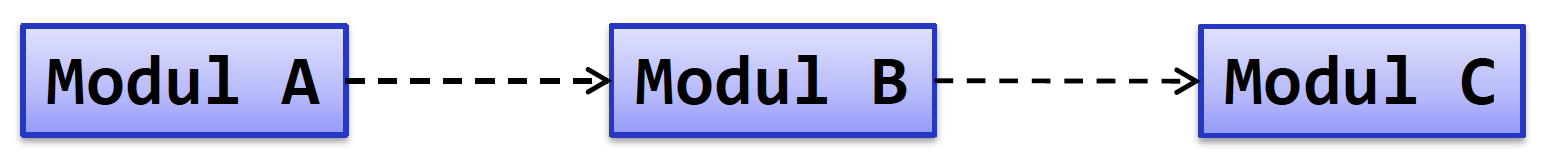
\includegraphics[keepaspectratio, height=1cm]{img/dependencymanagement/transitive_dependencies.png}
			\caption{Transitive Abhängigkeit zwischen 3 Modulen}
			\label{fig:transitive}
		\end{figure}
	
		Auflösung der Dependencies:
		\begin{itemize}
			\item \textbf{Modul A} ist von \textbf{Modul B} abhängig, dieses wiederum von \textbf{Modul C}
			\item \textbf{Modul A} ist also transitiv auch von \textbf{Modul C} abhängig
			\item Für Kompilation wird also \textbf{Model C} auch benötigt\\
			
			\item Durch direkte \& transitive Abhängigkeiten können auch Konflikte oder Zyklen auftreten.\\
			Maven erkennt und meldet diese, einfachere Konflikte können automatisch aufgelöst werden.
			\item Maven wertet die Dependencies als Graph aus, dient der Suche von Zyklen und Auflösung von Konflikten z.Bsp. über den kürzesten Pfad.
		\end{itemize}
	
	\subsection{Sie kennen das Versionskonzept und die Funktionsweise von Snapshots.}
	
	\begin{itemize}
		\item Einsatz von \textit{Semantic Versioning} wird empfohlen
		\item Einmal deployte Version kann im Optimalfall nicht mehr überschrieben werden\\
				$\rightarrow$ nachvollziehbare Buildprozesse
	\end{itemize}

			\paragraph{Semantic Versioning}
			
			\begin{itemize}
				\item \textbf{Major}-Release (\textbf{X}.x.x)\\
						Veränderungen in API, fachlicher Funktion und/oder in Konfiguration, welche zu früheren Versionen nicht kompatibel sind.
						Meist sind Anpassungen notwendig.
						
				\item \textbf{Minor}-Release (x.\textbf{X}.x)\\
						Erweiterungen in API, fachlicher Funktion oder Konfiguration, ist aber rückwärtskompatibel.
						Ohne Nutzung der Neuerungen keine Anpassungen notwendig.
						
				\item \textbf{Bugfix/Maintenance}-Release (x.x.\textbf{X})\\
						Reine Korrekturen in Änderungen oder Implementation, voll rückwärtskompatibel, keine neuen oder veränderten Funktionen.
						Direkter, sofortiger Einsatz möglich/notwendig (Bugfix)
			\end{itemize}
		
			\paragraph{Versionierung mit Snapshots}
			
			\begin{itemize}
				\item Version kann das Appendix \texttt{-SNAPSHOT} tragen.
				\item Gilt dann als erneuerbar und noch nicht stabil, sondern in Entwicklung
				\item Wird bei jedem \textbf{Build} vom Repo aufgelöst und aktualisiert
				\item Im Repo sind Snapshots mit Timestamp versehen
			\end{itemize}
	
		\subsubsection{Managed Dependencies in Multi-Modul-Projekten}
		
		\begin{itemize}
			\item Mehrere Submodule können von gleicher Dependency abhängig sein
			\item In jedem Modul sollte dieselbe Version verwendet werden
			\item \textbf{Lösung:} Im Master-POM über \texttt{dependencyManagement}-Element eine Liste an Dependencies (inkl. Version und Scope) als Baseline / Valid Version Set vordefinieren\\
			$\rightarrow$ Submodule müssen nur noch GroupId und ArtifactId angeben.
			Version und Scope werden vom Parent-POM vererbt.
			\item \textbf{\textit{Alternativ:}} Verwendung eines BOM (Bill of Material):\\
			Verschiedene Versionen werden in "virtueller" Release-Unit als "Baseline" referenziert.
			Lieferant bestimmt, welche zueinander passenden Versionen eingesetzt werden.
			Das BOM wird selber als Dependency definiert.
		\end{itemize}
	
	\subsection{Sie wissen auf welche Art Dependencies deployed werden}

	\begin{itemize}
		\item Häufigste Deployment-Art: JAR-Dateien
		\item Beispiel für ein Artefakt\\
				\texttt{ch.hslu.vsk:stringpersistor-api:4.0.1}:
			\begin{description}
				\item[POM (Metainfos)] \texttt{stringpersistor-api-4.0.1.\textbf{pom}}
				\item[JAR (Binary)] \texttt{stringpersistor-api-4.0.1.\textbf{jar}}
				\item[JavaDoc] \texttt{stringpersistor-api-4.0.1-\textbf{javadoc}.jar}
				\item[Source (bei OSS)] \texttt{stringpersistor-api-4.0.1-\textbf{sources}.jar}\\
			\end{description}
		
		\item Deployment in öffentliche Repos: sehr restriktiv\\
				$\rightarrow$ nichts mehr ändern, nichts löschen: Stabilität von Builds wahren!
		
		\item \textbf{Lösung:} nachvollziehbarer, automatisierter, verifizierbarer Release-Prozess, welcher von einem Build-Server ausgeführt wird
	\end{itemize}
	
	\newpage	
	\section{Versionskontrollsysteme - Source Code Management (SCM) / Version Control Systems (VCS)}
	
		\subsection{Sie kennen die Aufgaben eines Versionskontrollsystems und können grundlegend damit arbeiten}
		\textbf{Grundlegende Arbeit:}
		\begin{description}
			\item[checkout] lokale Arbeitskopie eines Projekts erstellen
			\item[update] Änderungen Dritter in Arbeitskopie aktualisieren
			\item[log] Bearbeitungsgeschichte eines Artefakts ansehen
			\item[diff] verschiedene Revisionen miteinander vergleichen
			\item[commit / checkin] Artefakte ins Repository schreiben $\rightarrow$ aussagekräftiger Kommentar!
		\end{description}
		\textbf{Tagging:} Revisionsstand mit Namen markieren, Marke oder Version: 1.5.2beta o.ä. Nützlich bei Release eines Produkts (aber auch meilensteine, Testversionen, Auslieferungszustände, etc.) wird unterschiedlich realisiert.\\
		\\
		\textbf{Branching:} Parallele, voneinander getrennte Entwicklungszweige (für Bugfixing, Prototypen, Tests, Experimente, nachvollziehbare Änderungsworkflows, etc.) Bei Nicht-Wegwerf-Entwicklungen später Merging möglich/notwendig.\\
		\\
		Ausschliesslich Quell-Artefakte werden verwaltet, \textbf{NIE} generierte/erzeugt Artefakte einchecken, können mit Hilfe der SCM ignoriert werden (.gitignore)
		
		\subsection{Sie kennen die verschiedenen Konzepte und Arten von Versionskontrollsystemen}
		\begin{itemize}
			\item Zentrale oder verteilte Systeme 
			\item Optimistische und pessimistische Lockverfahren 
			\item Versionierung auf Basis einer Datei, Verzeichnisstruktur oder der Änderung (changeset) 
			\item Transaktionsunterstützung (vorhanden oder nicht) 
			\item Verschiedene Zugriffsprotokolle und Sicherheitsmechanismen 
			\item Integration in Webserver (vorhanden oder nicht)
		\end{itemize}
		
		\subsection{Sie können mit verschiedenen (Client-)Werkzeugen von Versionskontrollsystemen alleine und im Team arbeiten}
		
		\begin{description}
			\item[CVS] UT-Versionskontrollsystem, stabil, wenig Fehler, einfache Anwendung, ABER nur dateibasierend, Verzeichnisstruktur nicht versioniert, unterscheidet zwischen Text- und Binärdateien, Ablage von Binärdateien platzintensiv, keine Transaktionen
			\item[Subversion] Transaktionsorieniert, versioniert ganze Verzeichnisstruktur, optimierte/effiziente Speicherung und Übertragung, Repositorystruktur frei wählbar (für Experten flexibler, für Anfänger schwieriger), Integration in Webserver möglich, aber Branching und Tagging technisch eig. Kopien/Links
			\item[git] verteiltes System, primär lokale Arbeit, beliebig viele Server/Repos möglich, auch rein lokal einsetzbar, skaliert, Integration mit zusätzlichen Web-Applikationen, erfordert aber ein solides Konzept, für Einsteiger schwierig, da sehr mächtig und viele Funktionen
		\end{description}
	
	\newpage
	\section{Testing Grundlagen}
		
		\subsection{Sie kennen die Motivation, den Sinn und den Zweck des Testens, was Sie mit Tests erreichen können und was nicht}
		
		\begin{quote}
			\textbf{Qualität} ist die Übereinstimmung mit den Anforderungen unter gleichzeitiger Einhaltung von Qualitätskriterien.
		\end{quote}
		\noindent
		Anforderungen müssen überprüfbar formuliert sein, typisch in Form von System- und Testspezifikationen.
		\textbf{Qualitätskriterien} sind: Funktionalität, Zweckdienlichkeit, Robustheit, Zuverlässigkeit, Sicherheit, Effizienz, Benutzbarkeit, Geschwindigkeit etc.
		Zur Überprüfung von diesen stehen uns Methodiken, Techniken, Vorgehensweisen etc. zur Verfügung.
		
		\begin{itemize}
			\item Wesentliche Tätigkeit ist das Testen - Qualitätssicherung durch Testen
			\item Wir überprüfen Verhalten eines Programms anhand der Spezifikationen
			\item Möglichst oft automatisiert teste, manuelles Testen ist aufwändig und zeitintensiv
			\item Begleitmassnahmen: Reviews, Entwicklungsprozess, Walkthrough, Metriken, Analysen, Regression, Automatisation etc.
		\end{itemize}
		
			\subsubsection{Welche Fehler können wir finden?}
			
			\begin{itemize}
				\item \textbf{Syntaktische Fehler:}\\
						Abweichungen von der Sprachsyntax (Schreibweise \& Grammatik) $\rightarrow$ formale Fehler.\\
						Diese werden durch Compiler aufgedeckt!
						\begin{itemize}
							\item Beispiel Sprache: \textit{"Der Lesr list ein Buck"}
							\item Beispiel Java: \texttt{if(i = 10) then{ i = 0; }}
						\end{itemize}
					
				\item \textbf{Semantische Fehler:}\\
						Abweichungen/Unstimmigkeiten, die auf Kenntnisse über Dinge beruhen $\rightarrow$ inhaltliche Fehler
						\begin{itemize}
							\item Beispiel Sprache: \textit{"Die Erdnuss ass einen Elefanten"}
							\item Beispiel Java: \texttt{double kelvin= celsius-273.15d;}
						\end{itemize}
					
				\item \textbf{Funktionale Fehler:}\\
						Abweichung von Anforderungen oder Erfüllung falscher/unerwünschter Anforderungen.\\
						Funktionale Fehler können \textbf{nur bedingt} durch Testen gefunden werden
						\begin{itemize}
							\item Beispiel: \textit{"Ein Liter Bier kostet ab jetzt 1000.-"}
						\end{itemize}
			\end{itemize}
			\vspace{1em}
			\noindent
			Testen ist systematisches, gezieltes  und möglichst effizientes "Durchprobieren" nach verschiedenen Qualitätskriterien.\\
			\textbf{Systematisch, gezielt} mit wohlüberlegten Eingabedaten / Testwerten\\
			\textbf{Effizient} möglichst aussagekräftige Tests durchführen\\
			Testen ist also \textbf{nicht} zielloses, chaotisches Pröbeln, sondern anspruchsvoller als man denkt.\\
			Man kann nur Vorhandensein von Fehlern, aber nie die Abwesenheit von Fehlern beweisen.
			Nach Test weiss man nur, dass ein Programm für die getesteten Eingabedaten korrekt läuft.\\
			$\rightarrow$ Eingabedaten so wählen, dass auf möglichst viele Varianten von möglichen Eingabedaten rückgeschlossen werden kann. 
			Also auch untypische Daten miteinbeziehen.\\
			Beispiel bei einem Sortieralgorithmus:
			\begin{itemize}
				\item beliebige, zufällige Daten (\textbf{Normalfälle})
				\item vorsortierte Daten, keine Daten (\textbf{Sonderfälle})
				\item ungültige, nicht sortierbare Daten (\textbf{Ausnahmefälle})
			\end{itemize}
			
			\begin{figure}[htb!]
				\centering
				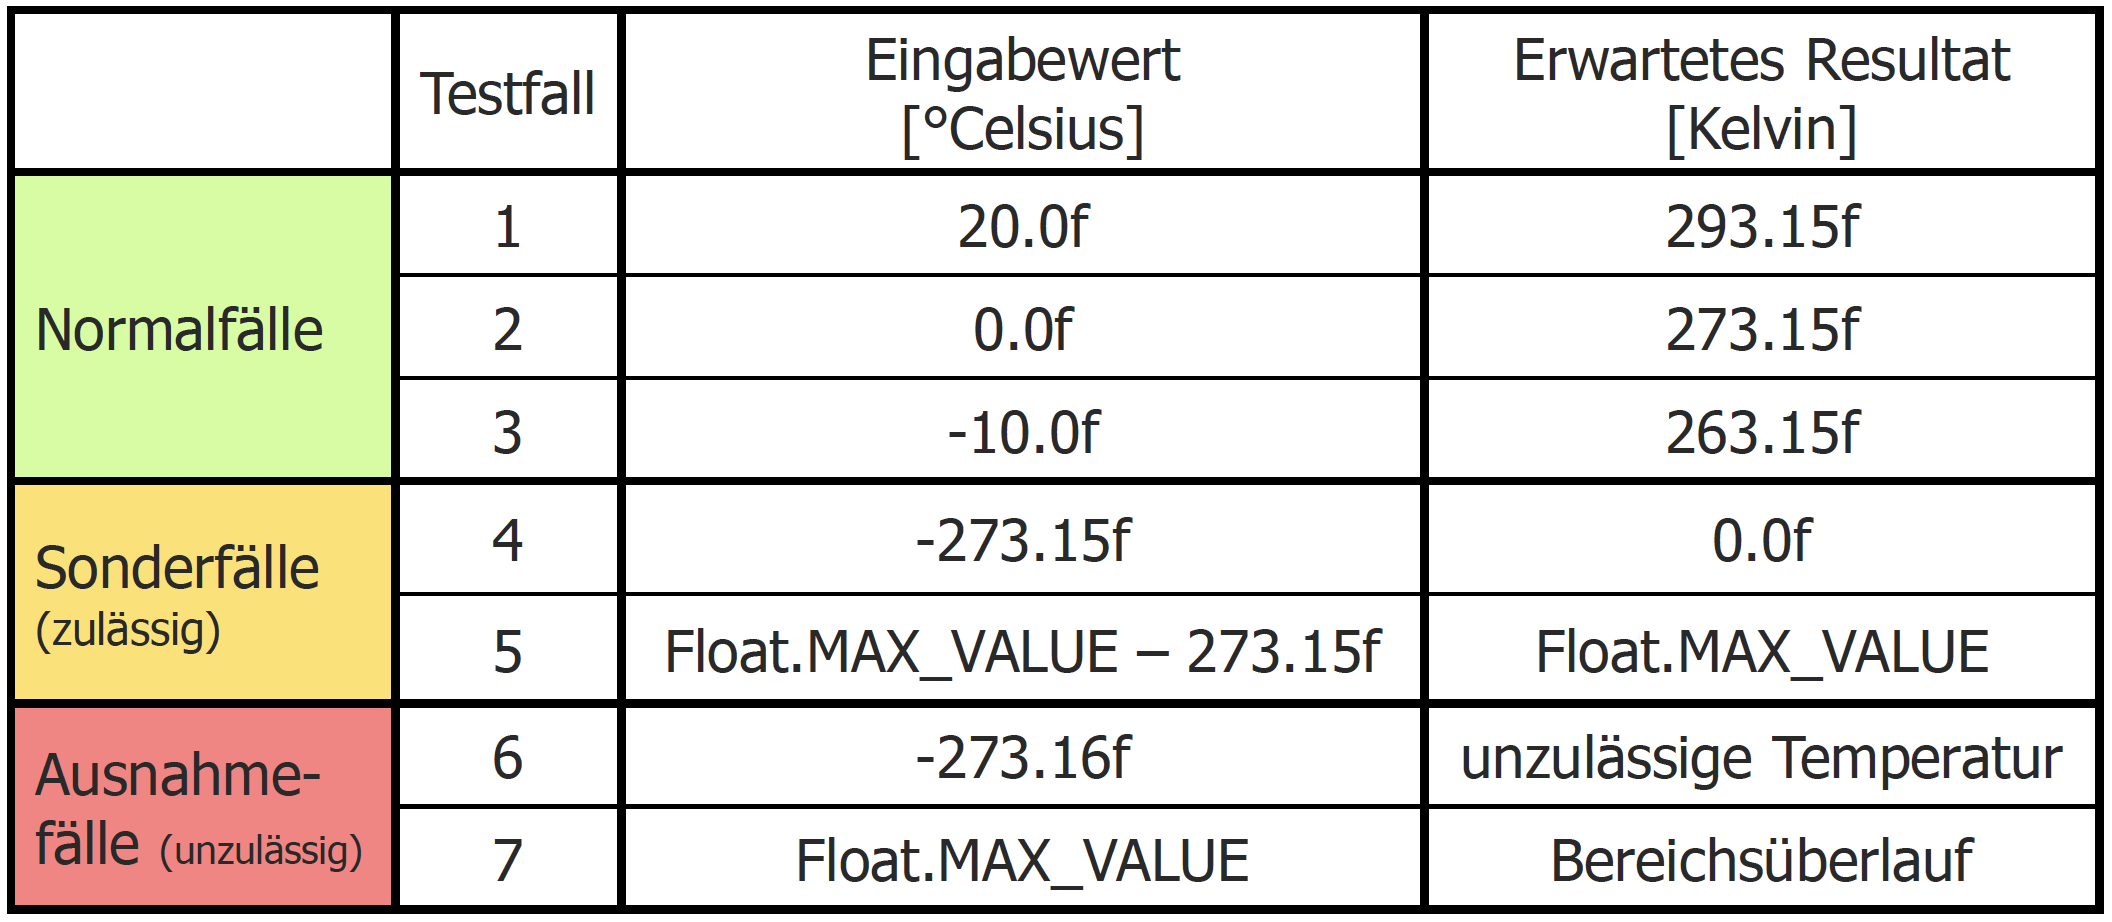
\includegraphics[keepaspectratio, height=3cm]{img/testing/planungstabelle.png}
				\caption{Tabelle für die Planung von Testfällen}
				\label{fig:table_testing}
			\end{figure}
			
			
		
		\subsection{Sie kennen verschiedene grundlegende Testarten und –verfahren}
		
		\begin{itemize}
			\item \textbf{Unit Tests:}\\
				\textit{Nur eine Methode/Klasse/Einheit wird getestet}\\
					Sehr klein, übersichtlich, einfach, schnell ausführbar, einfach automatisierbar \\
					(Ausführung \& Validation)
					
			\item \textbf{Integrationstests:}\\
					\textit{Mehrere Klassen (Module/Teilsysteme) in ihrem Zusammenspiel werden getestet}\\
					Deutlich aufwändiger, aber auch automatisierbar
					
			\item \textbf{Systemtest:}\\
					\textit{Ganzes System (viele Klassen/Einheiten) wird getestet}\\
					Klassisches Testen, erst spät möglich, aufwändig, auch automatisierbar
					
			\item \textbf{Black}- und \textbf{White}-Box Testing:\\
					Testen \textbf{ohne} oder \textbf{mit} Kenntnis der Implementation
			
		\end{itemize}
		
		\subsection{Sie können in Ihrer Entwicklungsumgebung einfache und gute Unit Tests, basierend auf dem JUnit-Framework, implementieren und anwenden}
		
			\subsubsection{Unit Tests}
			
			\begin{itemize}
				\item Testfälle programmiert, somit automatisiert, jederzeit schnell ausführbar und wiederholbar
				\item Sind "self-validating": Automatische Verifizierung, ob Testfall erfolgreich ausgeführt wurde
				\item Getestete Einheiten: einzelne Methoden oder Klassen\\
						$\rightarrow$ Kleine, überschauliche Testfälle
				\item Zahlreiche Frameworks für Testing, sind gut in IDEs integriert\\
						$\rightarrow$ Für Java: JUnit, UnitNG etc.
			\end{itemize}
		
			Nutzen daraus:
			\begin{itemize}
				\item Zeitersparnis: einmal schreiben, n-mal ausführen
				\item Kein manuelles "Testen" mehr
				\item \texttt{System.out.println()}-Orgien entfallen
				\item Jederzeit reproduzierbar
				\item Automatische Verifizierung der Ergebnisse mit Reporting
				\item Testfälle "dokumentieren" erwartete Funktion/Resultat
				\item Freiheit, mit geringem Risiko Code zu verändern / umschreiben (Refactoring)
			\end{itemize}
		
			\subsubsection{JUnit Test Framework}
			
			\begin{itemize}
				\item Aktuelle Version ist JUnit 5
				
				\item JUnit wird heute für alle automatisierbaren Testfälle eingesetzt\\
						$\rightarrow$ \textit{Nicht jeder JUnit-Testfall ist ein Unit-Test!}
						
				\item JUnit 5 hat viele Verbesserungen, ist aber nicht rückwärtskompatibel (OMG ein Major-Release!)
			\end{itemize}
			\noindent
			Ein Testfall entspricht dem "Build-Operate-Check"-Pattern:
			\begin{enumerate}
				\item \textbf{Erstellen} der Testobjekte bzw. -daten
				\item \textbf{Manipulieren} der Testobjekte bzw. -daten
				\item \textbf{Verifikation} der Ergebnisse (mit \texttt{assert*}-Methoden)
			\end{enumerate}
			\vspace{1em}
			\noindent
			Auch bekannt als "Triple-A"-Pattern: \textbf{A}rrange, \textbf{A}ct, \textbf{A}ssert
			\begin{figure}[!htb]
				\centering
				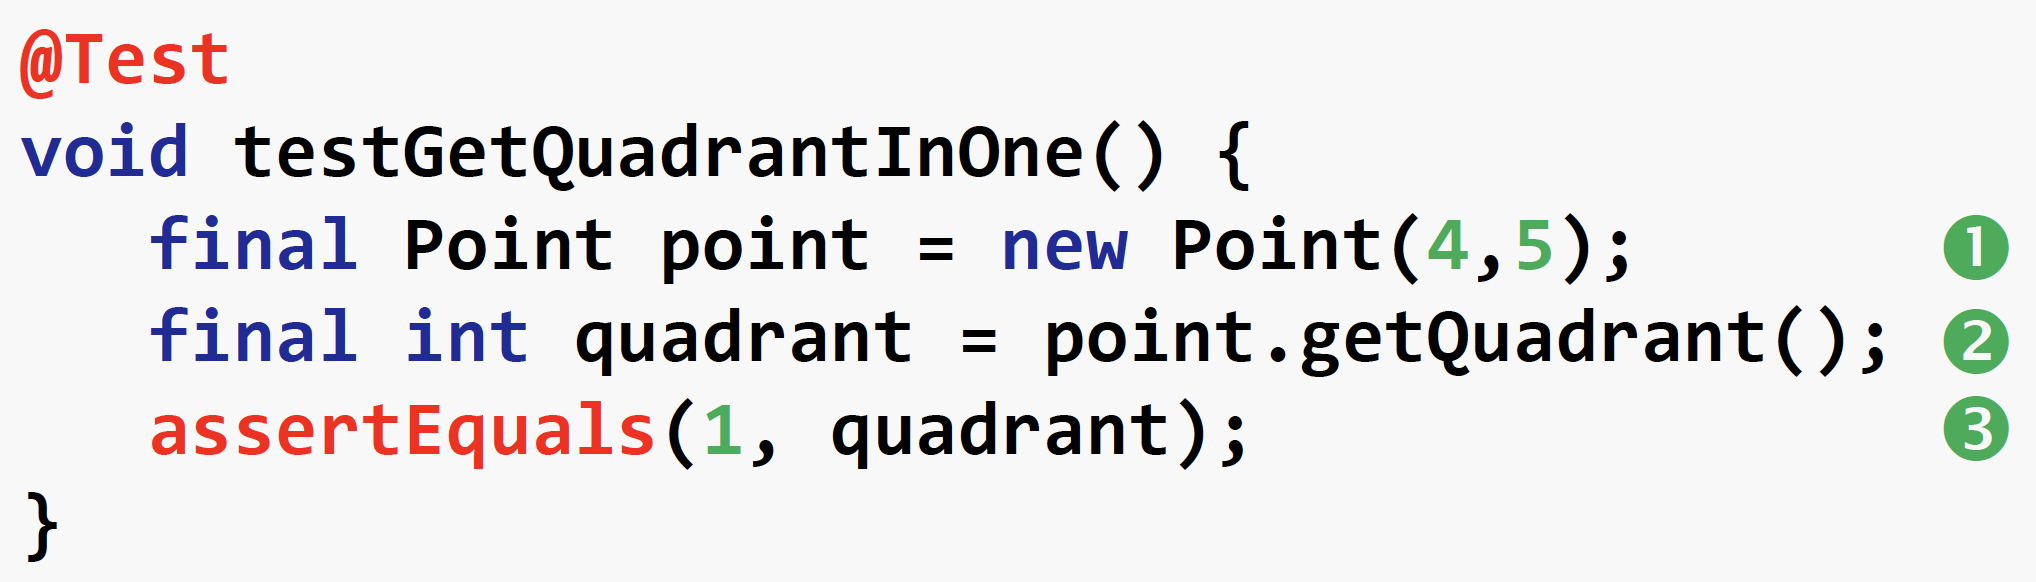
\includegraphics[keepaspectratio, height=3cm]{img/testing/test_01.png}
				\caption{Beispiel-Testfall}
				\label{fig:test_01}
			\end{figure}
		
				\paragraph{Self-Validating mit assert*-Methoden}
				
				Einfacher Vergleich zwischen einem Soll- und Ist-Wert, Methoden der Klasse \texttt{org.junit.jupiter.api.Assertions}, für viele Daten überladen (elementar oder Klasse \texttt{Object})
				
				\begin{figure}[!htb]
					\centering
					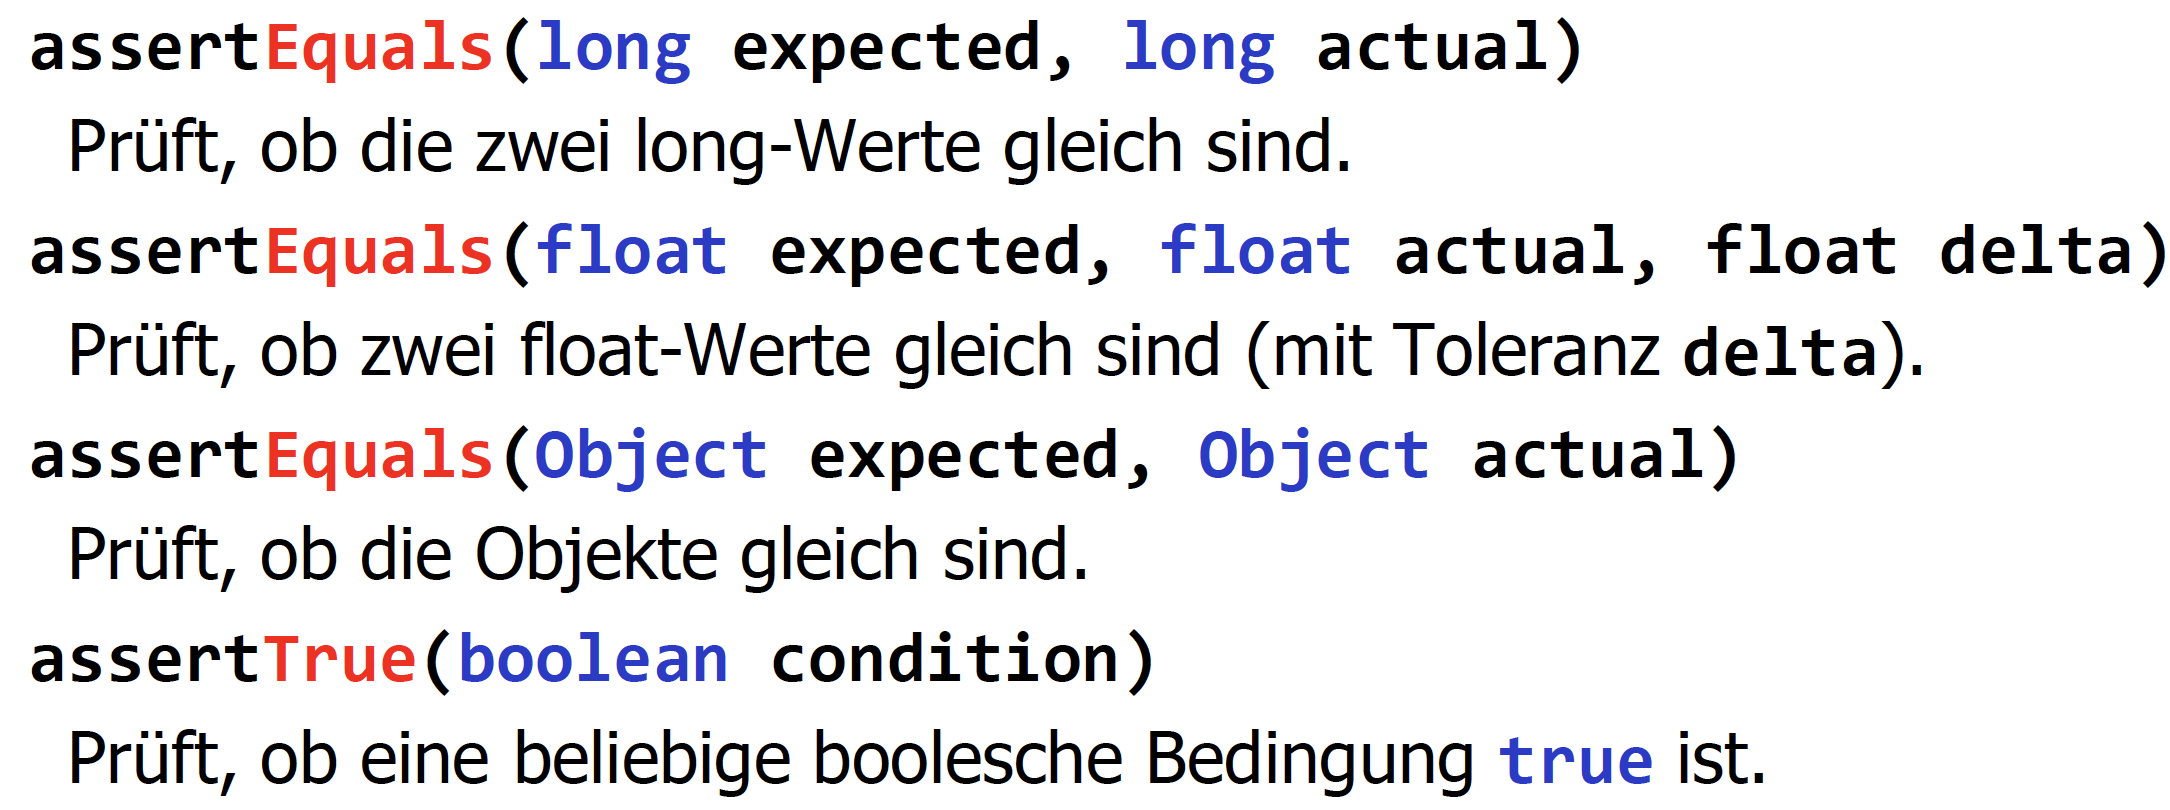
\includegraphics[keepaspectratio, height=3.5cm]{img/testing/test_asserts.png}
					\caption{Beispiele für assert*-Methoden}
					\label{fig:test_asserts}
				\end{figure}
			
				\paragraph{Annotations für Test-Methoden}
				
				Zur Konfiguration von Tests stehen mit JUnit verschiedene Annotationen zur Verfügung:
			
				\begin{figure}[!htb]
					\centering
					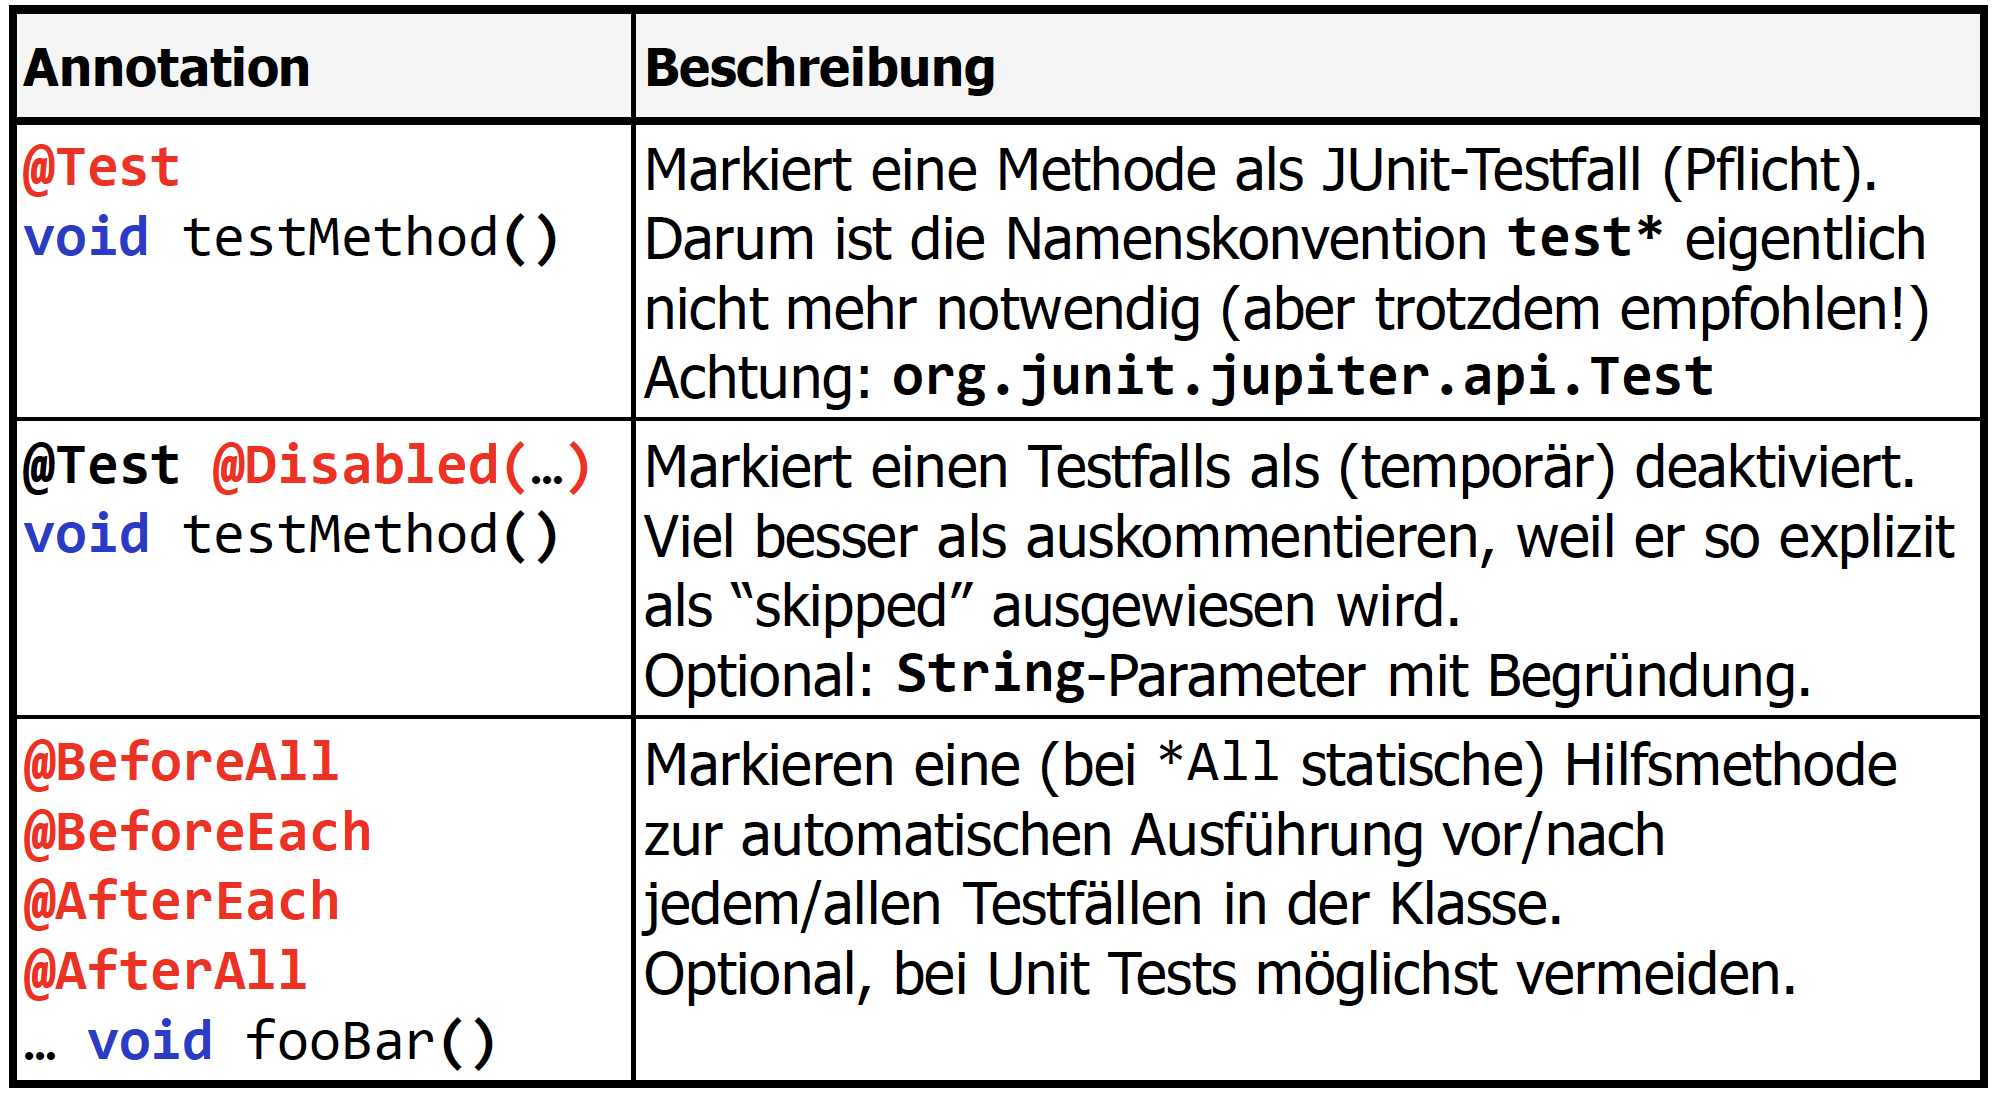
\includegraphics[keepaspectratio, height=5.5cm]{img/testing/test_annotations.png}
					\caption{Annotationen im Code für Testfälle}
					\label{fig:test_annotations}
				\end{figure}
			
				\paragraph{Namenskonventionen}
				
				\begin{itemize}
					\item \textbf{Testklasse:}\\
						Für Klasse \texttt{Demo}: \texttt{DemoTest}\\
						\texttt{Test} als Appendix, alle Testklassen ind \texttt{/src/main/test}!
					
					\item \textbf{Testmethoden:}\\
						Für Methode \texttt{foo(...)}: \texttt{testFoo[Xyz]()}\\
						\texttt{test} als Präfix, \texttt{Xyz} als freie, ergänzbare Fallbeschreibung, Testmethoden haben keine formalen Parameter
				\end{itemize}
			
			\subsubsection{Empfehlungen}
			
			\begin{itemize}
				\item Besser viele kleine Testmethoden als wenig grosse \\
				$\rightarrow$ im Fehlerfall bessere Selektivität
				
				\item Wenige \texttt{assert*}-Statements pro Testmethode \\
				$\rightarrow$ höhere Selektivität im Fehlerfall und übersichtlicher
				
				\item Methoden mit Rückgabewert am einfachsten testbar\\
				$\rightarrow$ Bei void-Methoden ggf. indirekt über Statusabfragen auf getestetes Objekt testen
				
				\item Getter \& Setter: gemeinsam oder indirekt "beiläufig" testen
				
				\item \textbf{Nie} Schnittstellen oder Sichtbarkeit nur für Testbarkeit ändern
				
				\item Klasse/Methode zu schwerig zu testen? $\rightarrow$ Hinterfrage mal deren Design...
			\end{itemize}
			
		\subsection{Sie kennen die Vorteile von Test First}
		
		Wir testen \textbf{kontinuierlich} während der Implementation, um von Beginn an Gewissheit zu haben, dass es funktioniert.\\
		Fehler finden, bevor man sie macht.
		Fehler finden, bevor man sie implementiert hat.
		Oder Fehler im Ansatz finden, bevor es jemand anders tut.
		Bullshitsätz...
		
			\subsubsection{Test First}
			
			\textbf{Immer vor der Implementation die Testfälle schreiben!}\\
			Vorteile dabei:
			\begin{itemize}
				\item Beim Schreiben der Testfälle denkt man automatisch an Implementation des zu testenden Codes\\
				$\rightarrow$ Implementation "reift" sozusagen beim Schreiben der Testfälle heran
				
				\item Ausnahmen und Sonderfälle fallen auf, welche bei der eigentlichen Implementation dann "automatisch" berücksichtigt werden
				
				\item Sobald die Komponente fertig implementiert ist, kann sie sofort getestet werden
			\end{itemize}
		
		\subsection{Code Coverage (Codeabdeckung)}
		
		\begin{itemize}
			\item Code Coverage = Metrik, welche zur Lauftzeit misst, welche Quellcodezeilen von Testfällen abgearbeitet wurden
			\item Wird typischerweise bei Ausführung der Unit-Testfällen (bspw. durch JUnit) durchgeführt\\
				$\rightarrow$ oder zur "normalen" Laufzeit, zur Messung welche Funktionen effektiv genutzt werden
			\item Ermöglicht eine Aussage, wie umfassend der Code getestet wurde\\
			(gezielte Effizienzsteigerung der Testfälle)
			\item Hohe Code Coverage ist \textbf{kein} Beweis für gute Testfälle oder Fehlerfreiheit!
		\end{itemize}
	
		\subsection{Unit Tests - Bilanz}
		
		\textbf{Positiv:}
		\begin{itemize}
			\item Testen ist vollständig in Implementationsphase integriert $\rightarrow$ Aufgabe des Entwicklers
			\item Neue / veränderte Methoden sind unmittelbar, reproduzierbar \& schnell testbar (regressiv)
			\item Test First: problemlos möglich und motivierend
			\item Automatisiertes, übersichtliches Feedback / Reporting
			\item Messung von Codeabdeckung integrierbar
		\end{itemize}
		\textbf{Negativ:}
		\begin{itemize}
			\item Qualität der Testfälle im Auge behalten $\rightarrow$ \textbf{Qualität vor Quantität}
			\item Für GUI(-Komponenten) aufwändiger
			\item In manchen Architekturen / Umgebungen schwierig umsetzbar
		\end{itemize} 
		
	\newpage
	\section{Automatisiertes Testing}
	
		\subsection{Sie kennen die verschiedenen Testarten und sind in der Lage gute Unit-und Integrationstests zu schreiben}
		
			\subsubsection{repeat(Unit Tests)}
			
			\begin{itemize}
				\item Häufig mit Komponenten/Modul/Entwickler-Tests gleichgesetzt
				\item Funktionale Tests von einzelnen, in sich abgeschlossenen Einheiten\\
						(typisch Klasse, aber auch Komponente oder Modul)
				\item Ziele von guten Unit-Tests:
					\begin{itemize}
						\item schnell, einfach ausführbar, selbstvalidierend (assert*-Methoden), automatisiert
						\item mögl. ohne Abhängigkeiten zu anderen Klassen/Komponenten/Modulen (lose Kopplung)
						\item Während Entwicklung geschrieben und ausgeführt (in IDE oder durch CI)
					\end{itemize}
				\item Gute Unterstützung durch Frameworks (JUnit, TestNG etc.)
			\end{itemize}
		
			\subsubsection{Integrationstests (JUnit)}
			
			\begin{itemize}
				\item \textbf{Namenskonvention:}\\
					\texttt{XyzIT} für Integrationstest (Klassenname + Appendix \texttt{IT})\\
					Ablegen unter \texttt{/src/test/java}
					
				\item Unterscheidung ergibt sich "nur" durch:\\
				Zeitpunkt der Ausführung, Laufzeit und Abhängigkeiten während der Ausführung
				
				\item Eigene Apache Maven Stage (\texttt{integration-test}) für Integrationstests\\
				Getrennte Plugins \texttt{surefire} und \texttt{failsafe} weisen Testresultate auch getrennt aus\\
				(Unit und Integration)
			\end{itemize}
		
			\subsubsection{Unit- vs. Integrationstests}
			
			\begin{itemize}
				\item \textbf{Unit-Tests} sind wirklich Unit-Tests, wenn sie auf beliebigem System und jederzeit lauffähig sind und (bei Java) auf unterschiedlichen Betriebssystemen laufen
				
				\item \textbf{Konsequenz:}\\
				Testfälle, die mit Dateisystem interagieren oder Sockets verwenden (auch wenn nur auf \texttt{localhost}), sind streng gesehen bereits Integrationstests
				
				\item Unit-Tests dürfen somit nie aufgrund von "Fremdeinflüssen" fehlschlagen\\
				(bspw. falscher Pfad, Platz, Zugriffsrechte etc.)
				
				\item \textbf{Empfehlungen:}
					\begin{itemize}
						\item Bewusst zwischen beiden Kategorien trennen
						\item Im Team auf gemeinsame Philosophie der Trennung der Kategorien einigen\\
						(Kann auch mal projektspezifisch sein)
						\item Je mehr als Unit Tests realisiert wird, desto besser
						\item Jeder automatisierte Test hilft
						\item Hilfsmittel wie Code Coverage oder Mocking nutzen
					\end{itemize}
			\end{itemize}
		
		
		\subsection{Sie nutzen Werkzeuge zur Messung der Codeabdeckung aktiv zu Verbesserung Ihres Codes und der Testfälle}
		
		Ja klar tu ich das!
		
		\newpage
		\subsection{Sie kennen das Prinzip der Dependency Injection}
		
		\begin{itemize}
			\item Schlechte Testbarkeit durch zu stark gekoppelte Abhängigkeiten\\
					$\rightarrow$ Schlechtes Design
			\item High-Level-Klassen sollen nicht von Low-Level Klassen abhängig sein, \\
			sondern beide von Interfaces
			\item Interfaces sollen nicht von Details, sondern Details von Interfaces abhängig sein!
			\item Isolation von Klassen, Auflösung von Abhängigkeiten durch Dependency Injection
			\item Dependency Inversion Principle - DIP (aus S.O.L.I.D.)
		\end{itemize}
	
			\subsubsection{Dependency Injection - Beispiel}
		
			Eine Klasse \texttt{PersonPersistor} soll implementiert werden, welche \texttt{Person}-Objekte als \texttt{String} serialisiert und in einer Datei speichert.
			Es existiert eine Implementation \texttt{StringPersistorFile}, welche wiederverwendet wird:
			
			\begin{figure}[!htb]
				\centering
				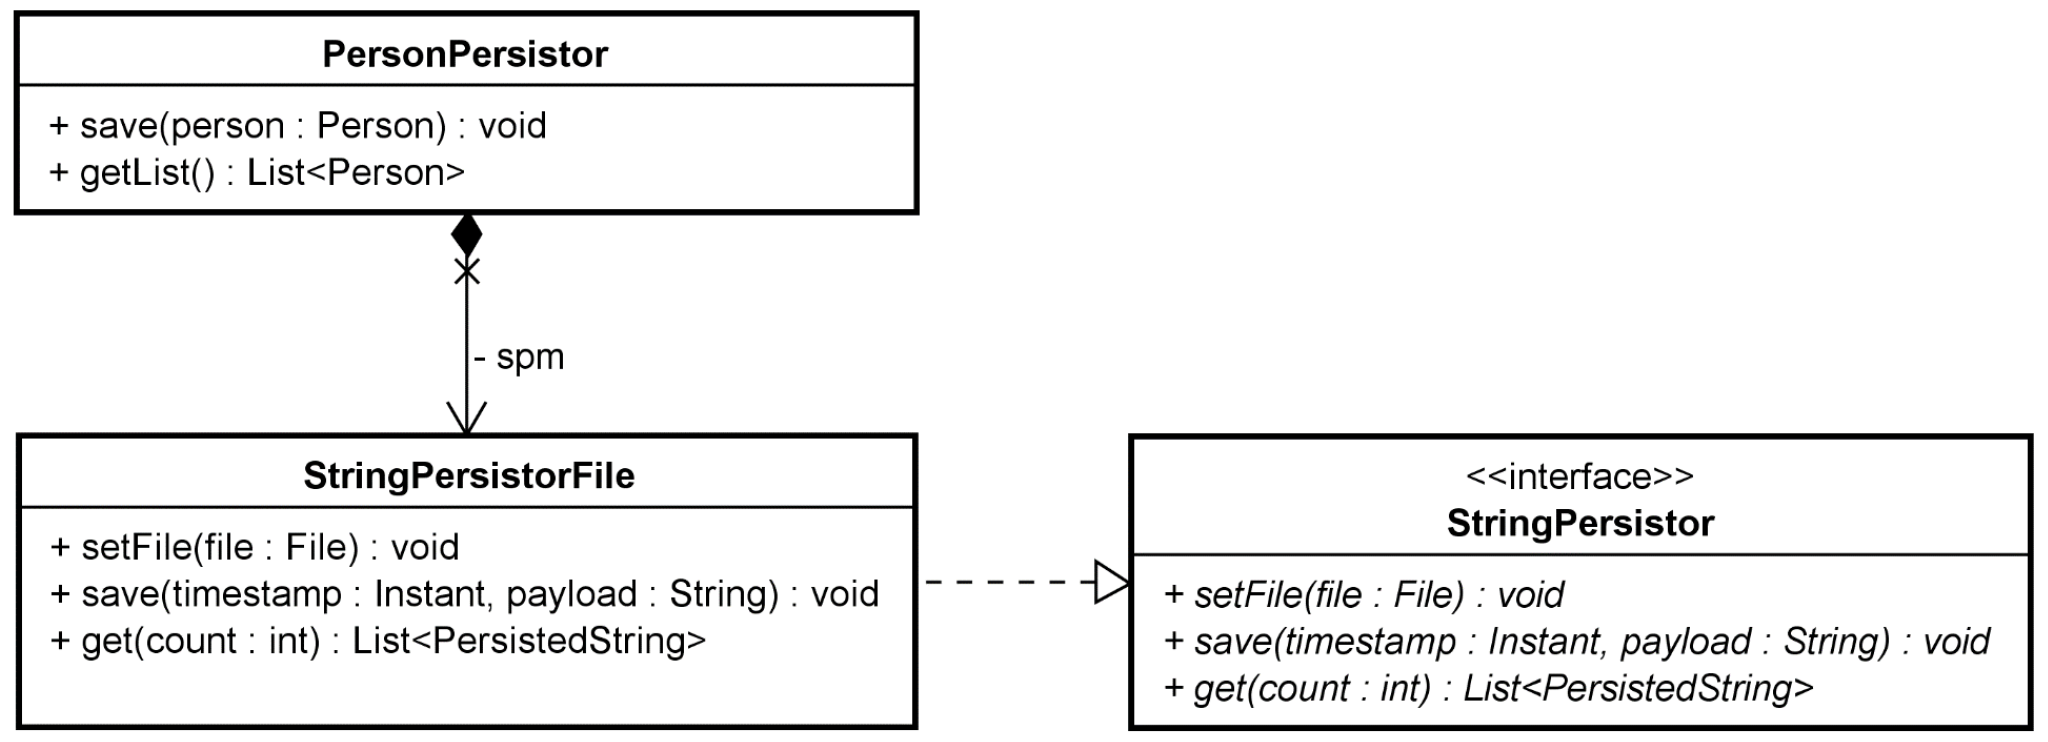
\includegraphics[keepaspectratio, height=5cm]{img/testing/di_01.png}
				\caption{Erster Lösungsansatz für das Problem}
				\label{fig:di_01}
			\end{figure}
			
			\textbf{EINE ZIEMLICH BEKNACKTE LÖSUNG FÜR TESTING!}\\
			
			\begin{lstlisting}
public final class PersonPersistor {
	private final StringPersistorFile spm = newStringPersistorFile();
	...
}
			\end{lstlisting}
			
			\begin{itemize}
				\item Einfach für die Realisierung, ist aber der einzige Vorteil, negative Aspekte:
					\begin{itemize}
					\item Typen und Implementation sind stark gekoppelt
					\item Abhängigkeit zur Implementationsklasse (obwohl ein Interface existieren würde)
					\item Unflexible Implementation
					\end{itemize}
				\item Wir wollen die Funktionalität der \texttt{PersonPersistor} testen, um Strings zu serialisieren und wieder zu deserialisieren
				\item \texttt{StringPersistorFile} greift aber auf das Dateisystem zu, weshalb die Abhängigkeit uns in die Kategorie der \textbf{Integrationstests} wirft\\
				Ausserdem würden wir den bereits getesteten \texttt{StringPersistorFile} nochmals testen\\
				$\rightarrow$ Selektivität des Testfalls sinkt
				\item Man müsste die Abhängigkeit auf den intern verwendeten \texttt{StringPersistorFile} durch etwas anderes ersetzen können
			\end{itemize}
			\vspace{1em}
			\noindent
			Lösung auf der nachfolgenden Seite
		
		\newpage
		
				\paragraph{Dependency Injection}
				
				Eine Klasse/Komponente erzeugt ihre Abhängigkeiten nicht selber, sondern lässt sich diese (wahlweise) auch von Aussen übergeben.
				
				\begin{figure}[!htb]
					\centering
					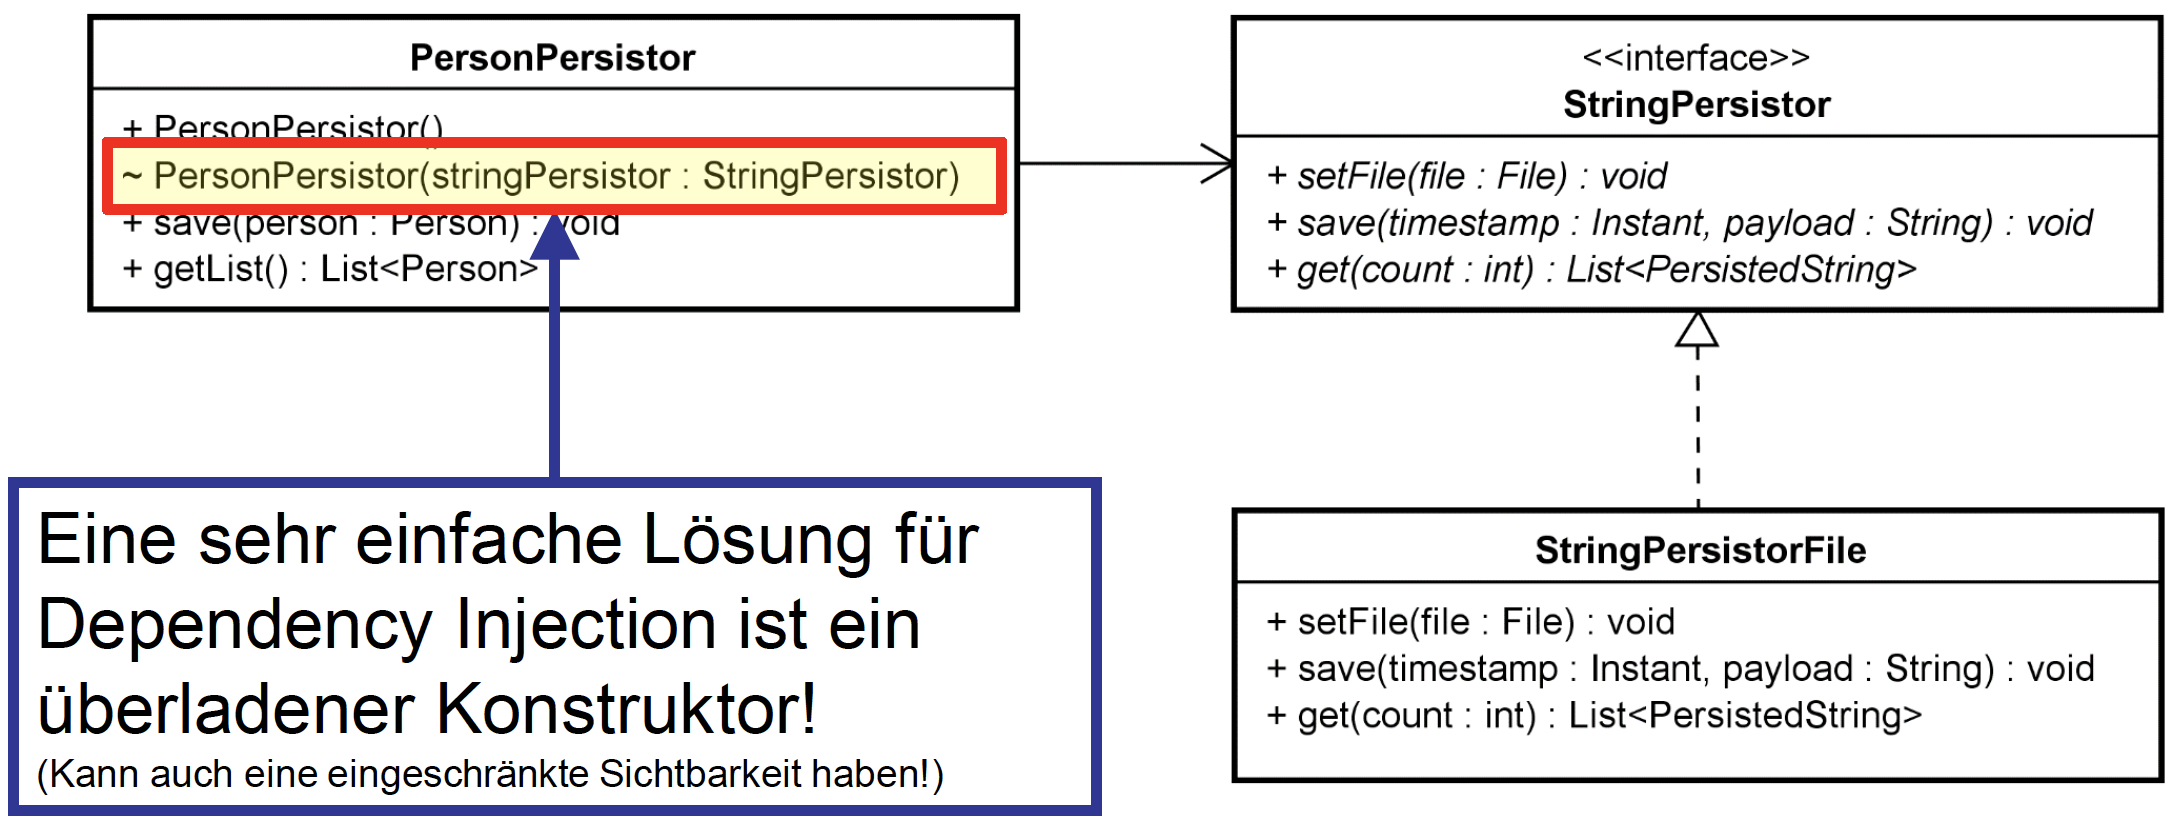
\includegraphics[keepaspectratio, height=5cm]{img/testing/di_02.png}
					\caption{Besserer Lösungsansatz für Testing mit Dependency Injection}
					\label{fig:di_02}
				\end{figure}
			
				\begin{itemize}
					\item Der konkrete Typ (Implementation) wird durch ein Interface ersetzt\\
					$\rightarrow$ Kopplung nimmt stark ab
					
					\item Es können so verschiedene, alternative Implementierungen genutzt werden\\
					$\rightarrow$ Andere Möglichkeiten / Ansätze testen
					
					\item Dependency Inversion Principle\\
					$\rightarrow$ Resultiert in besserer "Separation of Concerns"
					
					\item Testbarkeit wird massiv vereinfacht, man kann während Tests eine alternative Implementation als Platzhalter einfügen $\rightarrow$ \textbf{Test Double}
					
					\item Integrationstest werden wieder zu Unit Tests, schnellere \& selektivere Tests
				\end{itemize}
		
		\subsection{Sie wissen was Test Doubles sind und können Mocking-Frameworks einsetzen}
		
			\subsubsection{Test Doubles}
			
			\begin{itemize}
				\item "Double" ist Platzhalter für eine echte, produktive Implementation während des Tests
				\item Oberbegriff "Test Doubles" umfasst verschiedene, interessante Spezialisierungen
				\item Test Doubles sollen Aufwand für Integrationstests reduzieren, indem stattdessen mehr Testfälle als Unit-Tests realisiert werden
				\item Möglichst viel mit Unit-Tests prüfen, weil:
					\begin{itemize}
						\item Erste Teststufe, direkt bei Entwickler
						\item Schnell, häufig, überall lauffähig, vollständig automatisiert
						\item Hohe Selektivität der Testfälle
					\end{itemize}
				\item Test Doubles sind auch innerhalb von Integrationstests nützlich\\
					$\rightarrow$ Gezielte Isolation der Tests von einzelnen Integrationen (Abhäng. von anderen Systemen)
				\item Für Test Doubles muss gutes Design der Software vorliegen\\
					$\rightarrow$ Einsatz von Interfaces lohnt sich (fast) immer, da ein Interface verschiedene Implementationen zulässt, minimum eine "echte" und eine Test-Implementation
				\item Wahl der Implementation muss zur Test-Laufzeit beeinflusst werden können\\
					$\rightarrow$ per Dependency Injection (manuell oder per Framework)\\
					(\textbf{Achtung:} Sicherung nötig, dass das nicht in der \textbf{Produktion} passiert)
			\end{itemize}
		
		\newpage
		
			\begin{figure}[!htb]
				\centering
				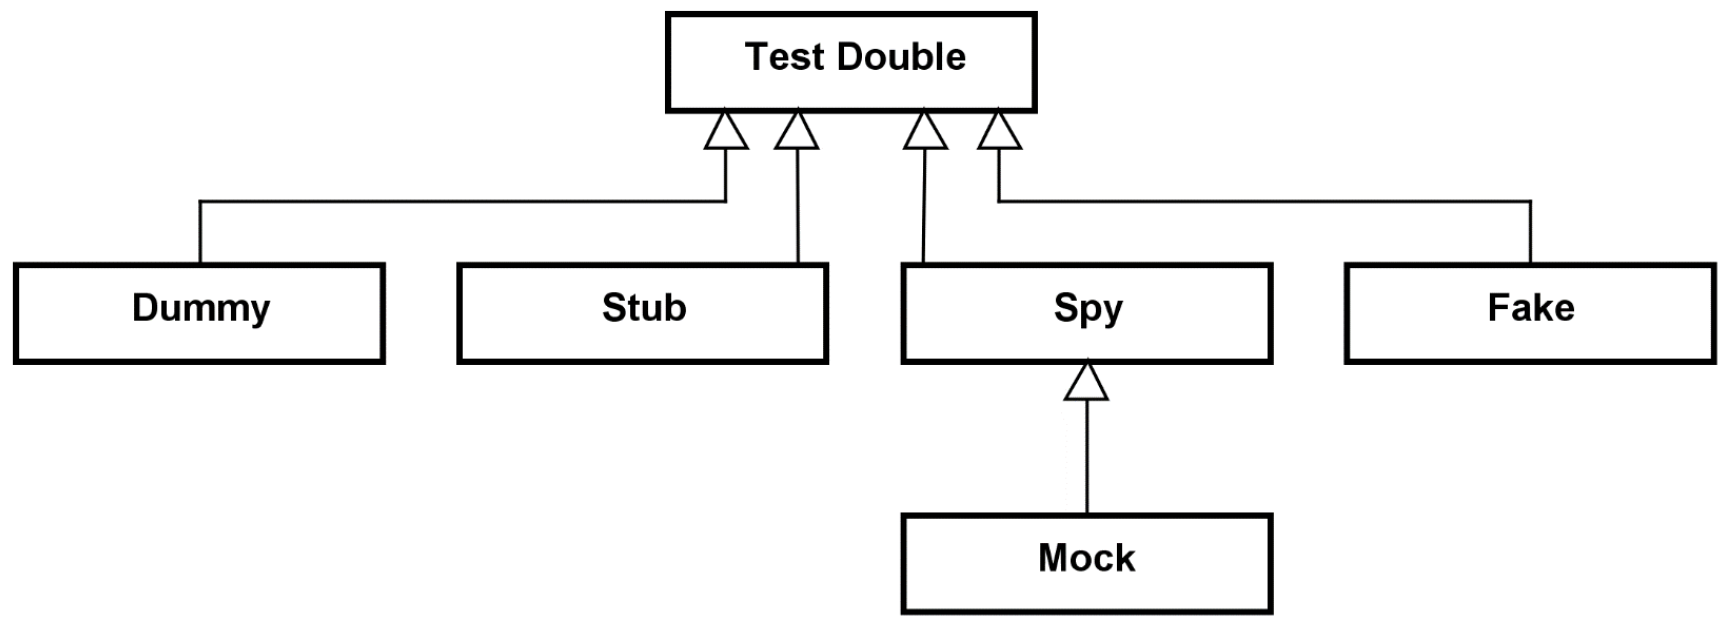
\includegraphics[keepaspectratio, height=4cm]{img/testing/doubles.png}
				\caption{Übersicht über alle verfügbaren Test-Doubles}
				\label{fig:doubles}
			\end{figure}
		
			\paragraph{Dummy}
			
				\begin{itemize}
					\item Sehr primitive, leere Ersatzimplementation, wird als aktueller Parameter an Methoden übergeben\\
					$\rightarrow$ Aktueller Parameter ist zwar notwendig für Test, dessen Nutzung und Implementation (für Test) aber irrelevant
					\item Dummy: dient funktionsloser Entkopplung der beim Test unerwünschten Abhängigkeiten
				\end{itemize}
				\begin{quote}
					\textbf{Beispiel:}\\
					Einem Objekt muss bspw. ein Logger übergeben werden.
					Dieser soll aber nichts machen, da Loggen nicht das eigentliche Testziel ist.
				\end{quote}
		
			\paragraph{Stub}
			
				\begin{itemize}
					\item Einfache Implementation, die mit möglichst geringem Aufwand sinnvolle, vordefinierte Werte (bspw. Konstanten)zurückliefert
					\item Erlaubt sogenanntes "State"-Testing\\
						$\rightarrow$ State durch Daten repräsentiert, State bei Stubs in der Regel konstant
					\item Für verschiedene Testziele ggf. auch mehrere untersch. Stubs erstellen
				\end{itemize}
				\begin{quote}
					\textbf{Beispiel:}\\
					Eine Klasse für Authentifizierung testen, welche...\\
					- Beliebige Nutzer/Passwörter akzeptiert: \texttt{login = true}\\
					- Niemanden akzeptiert: \texttt{login = false}
				\end{quote}
			
			\paragraph{Spy}
			
				\begin{itemize}
					\item Alternative Implementation, welche dynamische Werte zurückliefern kann.
					Der Spy merkt sich gleichzeitig auch die Aufrufe der Methode\\
					(Anzahl/Häufigkeit, Paramater, Zeitpunkt, Exceptions etc.)
					\item Nach Interaktion können aufgezeichnete Ereignisse zur Verifikation des Testfalls genutzt werden.
					\item Erlaubt "Behavior"-Testing (Verhalten)
				\end{itemize}
				\begin{quote}
					\textbf{Beispiel:}\\
					Wurde auf dem beim Testkandidaten registrierten \texttt{ActionListener}(-Spy)\\
					die Methode \texttt{actionPerformed()} auch tatsächlich aufgerufen?
				\end{quote}
			
			\paragraph{Mock}
			
				\begin{itemize}
					\item Spezialisierung des Spy, welcher dynamische Werte zurückliefern kann und die korrekte Interaktion selber verifizieren kann $\rightarrow$ Abgrenzung zum Spy
					\item Typisch mithilfe von Mock-Frameworks zur Laufzeit für jeden Testfall als individuelle Mock-Objekte erstellt (Proxy-Pattern, GoF)\\
					$\rightarrow$ Verhalten für jeden Testfall dynamisch / programmatisch konfiguriert
					\item Sehr ähnlich zu Spy, Unterschied ist jedoch der Ort der Verifikation, Mocks sind spezifischer
				\end{itemize}
			
			\newpage
			
			\paragraph{Fake}
			
				\begin{itemize}
					\item Alternative Implementation, welche eine Komponente \\
					mit vernünftigem Aufwand vollständig ersetzen kann
					\item Ermöglicht vollständige Entkopplung von einer Abhängigkeit\\
						Trade-Off $\rightarrow$ Aufwand der Implementation des Fake muss in vernünftigem Verhältnis zum Nutzen sein (Unit vs. Integration)
				\end{itemize}
				\begin{quote}
					\textbf{Beispiel:}\\
					Abhängigkeit von Webservices durch lokale Fake-Implementation ersetzt\\
					- Kommunikation fällt weg, ist somit schneller\\
					- Implementation trotzdem vorhanden (wenn nicht zu komplex), \\
					idealerweise auch wiederverwendet
				\end{quote}
		
		\subsubsection{Effektives Testen mit Test Doubles - Beispiele}
		
		\textbf{Mockito} - bewährtes Testing-Framework für Java.\\
		In Maven einbinden mit \texttt{org.mockito:mockito-core:2.23.0}\\
		Viele statische Klassen auf der Klasse \texttt{org.mockito.Mockito}.\\
		Bestenfalls statischer Import aller Funktionen:\\
		\texttt{import static org.mockito.Mockito.*;}
		
		\paragraph{Test mit Fake}
		
			Für Testausführung wird Fake-Implementation \texttt{StringPersistorMemory} (statt \texttt{File}) verwendet, welche Strings nur im Memory "speichert":
			
			\begin{lstlisting}
@Test
public void testGetEmptyList() {
	final Person Persistorinstance = 
		new PersonPersistor(new StringPersistorMemory());
	assertThat(instance.getList()).isEmpty();
}
			\end{lstlisting}
			\noindent
			Für diesen Testfall resultiert:
			\begin{itemize}
				\item Keine Abhängigkeit mehr zum Dateisystem
				\item Unit-Test (kein Integrationstest)
				\item Testet viel weniger Dritt-Code und wird damit selektiver
			\end{itemize}
		
		\paragraph{Test mit Mock}
		
			Für Testausführung wird Mock (oder Spy) verwendet, welcher direkt im Testfall erzeugt / konfiguriert wird:
			
			\begin{lstlisting}
@Test
public void testGetEmptyList() {
	finalStringPersistor mock = 
									mock(StringPersistor.class);
	when(mock.get(0)).thenReturn(Collections.emptyList());
	finalPersonPersistorinstance = 
									newPersonPersistor(mock);
	assertThat(instance.getList()).isEmpty();
}
			\end{lstlisting}
			\noindent
			Der Testfall:
			\begin{itemize}
				\item Keine Abhängigkeit mehr zu einer Implementation
				\item Selektivität ist maximal
			\end{itemize}
				
		\newpage
		
		\subsubsection{Empfehlungen}
		
		\begin{itemize}
			\item Gewisse Klassen sind zu aufwändig für Mocking
			\item Gewisse Klassen sind zu einfach für Mocking
			\item Verständlichkeit des Testcodes am wichtigsten, wenn Testfall durch Mocking zu kompliziert wird, dass man ihn nicht mehr versteht, hed mer huere verlore.
			\item Überleged si sich öbs sich lohnt. Stiiged si doch langsam id Technik ii, si esch absolut faszinierend!\\
			\textit{- Roli Gisler}
		\end{itemize}
	
			\paragraph{Wann setzt man was ein?}
			
			\begin{itemize}
				\item \textbf{Dummy / Stub:}\\
				Einfache Ersatzimplementationen, um bessere Testisolation zu erreichen\\
				Geringer Aufwand $\rightarrow$ höhere Selektivität / Stabilität der Testfälle (einfach)
				
				\item \textbf{Spy / Mock:}\\
				"Universalwaffen" für Behavior-Testing mithilfe Mocking-Frameworks.
				Können auch zur Realisierung von Stubs / Dummies genutzt werden (komplexer)
				
				\item \textbf{Fake:}\\
				Aufwändige Implementation, zur vollständigen Entkopplung vom Original.\\
				Muss sich lohnen (aufwändig)\\
				(Ja aber was wänn de Fake besser isch as de Original..??)\\
				
				\item Design ist entscheidend:\\
				So oft wie möglich Interfaces verwenden, um schneller alternative Implementationen zu integrieren
			\end{itemize}
				
	\newpage
	\section{Software Architektur}
		
		\subsection{Sie können den Begriff «Software Architektur» einordnen}
		
		\begin{itemize}
			\item Eine Architektur ist eine Abstraktion, etwas wird zusammenfassend/vereinfacht dargestellt\\
			$\rightarrow$ vergleiche Modellierung
			\item Architektur beschreibt ein System durch:
				\begin{itemize}
					\item \textbf{Struktur und Aufbau:}\\
							Sub- \& Teilsysteme, Schichtung, "Zwiebel", Verteilung
					\item \textbf{darin enthaltene Softwareteile:}\\
							Gegliedert nacht Aufgaben, Zuständigkeiten, Komponenten, aber auch Technologien
					\item \textbf{deren Beziehungen untereinander:}\\
							Abhängigkeiten, Schnittstellen, Datenflüsse, Deployment
				\end{itemize}
		\end{itemize}
	
			\paragraph{Definitionen zu Architektur}
			
				\begin{quote}
					\textit{«Softwarearchitektur definiert sich durch die Kernelemente eines Systems, welche als Basis für alle weiteren Teile nur schwer und aufwendig verändert werden können.»}\\
					- Martin Fowler
				\end{quote}
				\begin{quote}
					\textit{«Die Architektur repräsentiert die signifikanten Designentscheidungen die ein System festhalten, wobei die Signifikanz an den Kosten von Änderungen bemessen wird.»}\\
					- Grady Booch
				\end{quote}
			
		\subsection{Sie haben eine Vorstellung, welche Informationen und Artefakte eine Software Architektur beschreiben}
		
			\subsubsection{Übersicht über Aspekte der Softwarearchitektur}
			
				\begin{itemize}
					\item Grundlegende Struktur
					\begin{itemize}
						\item Schichten, Client / Server, n-tiers etc.
						\item Architekturmuster
					\end{itemize}
					\item Kommunikation \& Verarbeitung
					\begin{itemize}
						\item Kommunikationsmuster (bspw. synchron / asynchron)
						\item Verteilbarkeit, Parallelität, Performance, Robustheit, Resilienz
					\end{itemize}
					\item Eingesetzte Technologien
					\begin{itemize}
						\item Userinterface (Fat-, Rich- oder Thin-Client)
						\item Persistenz der Daten
						\item Referenzarchitekturen
					\end{itemize}
					\item Qualitätsaspekte
					\begin{itemize}
						\item Wartungsfreundlichkeit, Erweiterbarkeit etc.
					\end{itemize}
				\end{itemize}
			
			\subsubsection{Motivation für (gute) Architektur}
			
				\begin{itemize}
					\item Explizite Architektur macht ein System erst "verstehbar".
					Fundamentale Grundlage für die Diskussion, Planung, Implementation und Betrieb eines Softwaresystems.
					
					\item Unmittelbare Qualitätsaspekte:
					\begin{itemize}
						\item bessere Wartbarkeit (Bugfixing)
						\item höhere Wiederverwendbarkeit
						\item leichte Erweiterbarkeit
						\item grössere Sicherheit
						\item vereinfachte Testbarkeit
						\item höhere Stabilität \& Robustheit
					\end{itemize}
					
					\item Auswirkung dieses Qualitätsaspekte:\\
					Verkürzung der time-to-market, echte Agilität
				\end{itemize}
				
			\newpage	
		
			\subsubsection{Architekturmuster und -stile}
			
			\begin{itemize}
				\item Konzepte, beschreiben Grundaufbau eines ganzen Systems\\
				(Vergleich: Entwurfsmuster sind (objektorientierte) Konzepte für einzelne Teilprobleme)
				
				\item Architekturmuster für verschiedene zentrale Aspekte/Schwierigkeiten in Softwarearchitektur:\\
				für (grosse, komplexe), (stark) verteilte, inter(re)aktive etc. Systeme, diese zu strukturieren\\
				Beispiele: Client/Server, peer-to-peer etc.
				
				\item Typisch nicht so stark vereinheitlicht \& standardisiert wie Entwurfsmuster
				
				\item Sehr viele Architekturstile hab sich im Laufe der Zeit entwickelt.
				Je nach Applikationsart erweisen sich diese als sehr schlecht oder gut brauchbar.
				
				\item \textbf{Erkenntnis 1:}\\
				Führte oft zum "FAT-Client" (Geschäftslogik im Client) und einer überforderten Datenbank\\
				Vorteil: zentrale Datenhaltung, hohe Konsistenz (RI, Trigger, SP)\\
				Nachteil: Transaktionen, Locking, Ressourcen, Verteilung etc.
				
				\item \textbf{Erkenntnis 2:}\\
				"Im Kleinen" bspw. für lokale (Einbenutzer-)Apps auf Handys funktioniert das gut.
				
				\item \textbf{Wahre Kunst:} Richtige Applikation am richtigen Ort!
			\end{itemize}
		
				\paragraph{Fliessender Wechsel zw. Design und Architektur}
				
				Grosse Palette an "altbekannten" Mustern, Prinzipien \& Techniken:
				Modularisierung von Komponenten, Schnittstellen, Packages;
				Gruppierung dieser zu (Sub-)Systemen;
				Nutzung versch. Muster zur Strukturierung (bspw. MVC - Model View Control, Schichtenbildung etc.).
				\textbf{Herausforderung:} All diese Prinzipien auf den unterschiedlichen Abstraktionsebenen angemessen zu befolgen und zu beurteilen.
				Schlussendlich haben wir «nur» einen Haufen von Klassen und Schnittstellen - jede weitere Strukturierung ergibt sich weitgehend nur durch Organisation und Konventionen!
				
			\subsection{Versch. Arten von Applikationen}
			
			\begin{itemize}
				\item Einzelbenutzerapplikation:\\
				Eher klein, evtl. nur Mobile App, lokale Persistenz, wenig komplexe Funktionalität
				\item Mehrbenutzerapplikation:\\
				bspw. Unternehmensapplikation, zentrale Services \& Daten, beliebige Komplexität, typisch in mehrere (Teil-)Systeme aufgebrochen.
				\item Internetanwendungen:\\
				Typisch mit Web-GUI, beliebig viele Benutzer, verteilte Datenspeicherung, beliebige Komplexität\\
				
				\item Sehr unterschiedliche Anforderungen an Architektur!
			\end{itemize}
		
		\subsection{Sie verstehen, dass die Bildung von Schichten eine fundamentale Basis für die meisten Architekturen ist}
		
		\begin{itemize}
			\item \textbf{Schichten (Layers):} Gliederung eines Systems\\
			in aufeinander aufbauende, funktional getrennte Schichten
				\begin{itemize}
					\item Kommunikation zw. Schichten über Schnittstellen
					\item Abhängigkeit nur in Richtung der tieferliegenden Schicht
				\end{itemize}
			\item Zur Strukturierung, innerhalb eines Systems \& systemübergreifend
			\item Mögliche physische Verteilung der Schichten: Schichten $\rightarrow$ Tiers
		\end{itemize}
	
		\newpage
		
			\subsubsection{Schichtenbildung}
			
			\begin{itemize}
				\item Bildung nach versch. Kriterien:\\
				Logisch / Funktional, Technik, Abstraktionsebene etc.
				\item Kann hierarchisch verfeinert werden:
					\begin{enumerate}
						\item funktionale Schichtung
						\item Abstraktionslevel
						\item Technologie
					\end{enumerate}
				\item Implementation mit Java:\\
				Schichten manifestieren sich in Modul- und Packagestruktur:\\
				\texttt{ch.domain.system.server} \& ch.domain.system.server\\
				\textit{(Kann schlechter Ansatz sein, vergleiche "package by feature")}
			\end{itemize}
	
				\paragraph{Schnittstelle zw. Schichten}
				
					\begin{itemize}
						\item Explizite Schnittstellen zw. Schichten $\rightarrow$ siehe \textit{Modularisierung}
						\item Erlauben Entkopplung von der konkreten Implementation, die ausgetauscht werden kann \\
						$\rightarrow$ auch die vollständige Schicht
						\item \textbf{Achtung:} zwischen Schichten ausgetauschte Daten sind Bestandteil der Schnittstelle und tragen zur impliziten Kopplung bei
							\begin{itemize}
								\item nützt nichts, wenn wir identische Datenobjekte über alle Schichten hinweg jagen
								\item Entscheid nötig, bei welchen Schichten wir Schnittstellen auch über Datentypen brechen
							\end{itemize}
					\end{itemize}
			
				\paragraph{Verteilte Schichten auf Tiers}
				
					\begin{itemize}
						\item Schichtenbildung:\\ 
						Fundamentale Grundlage zur Realisierung von verteilten Anwendungen / Architekturen
						\item Schichtengrenzen:\\ 
						Eignen sich gut zur Auftrennung, um Teile auf verschiedene Systeme zu deployen / verteilen
						\item Werden Schichten auch physisch getrennt, spricht man von Tiers\\
						(Client / Server-Beziehung zwischen Schichten)
					\end{itemize}
				
					\begin{figure}[!htb]
						\centering
						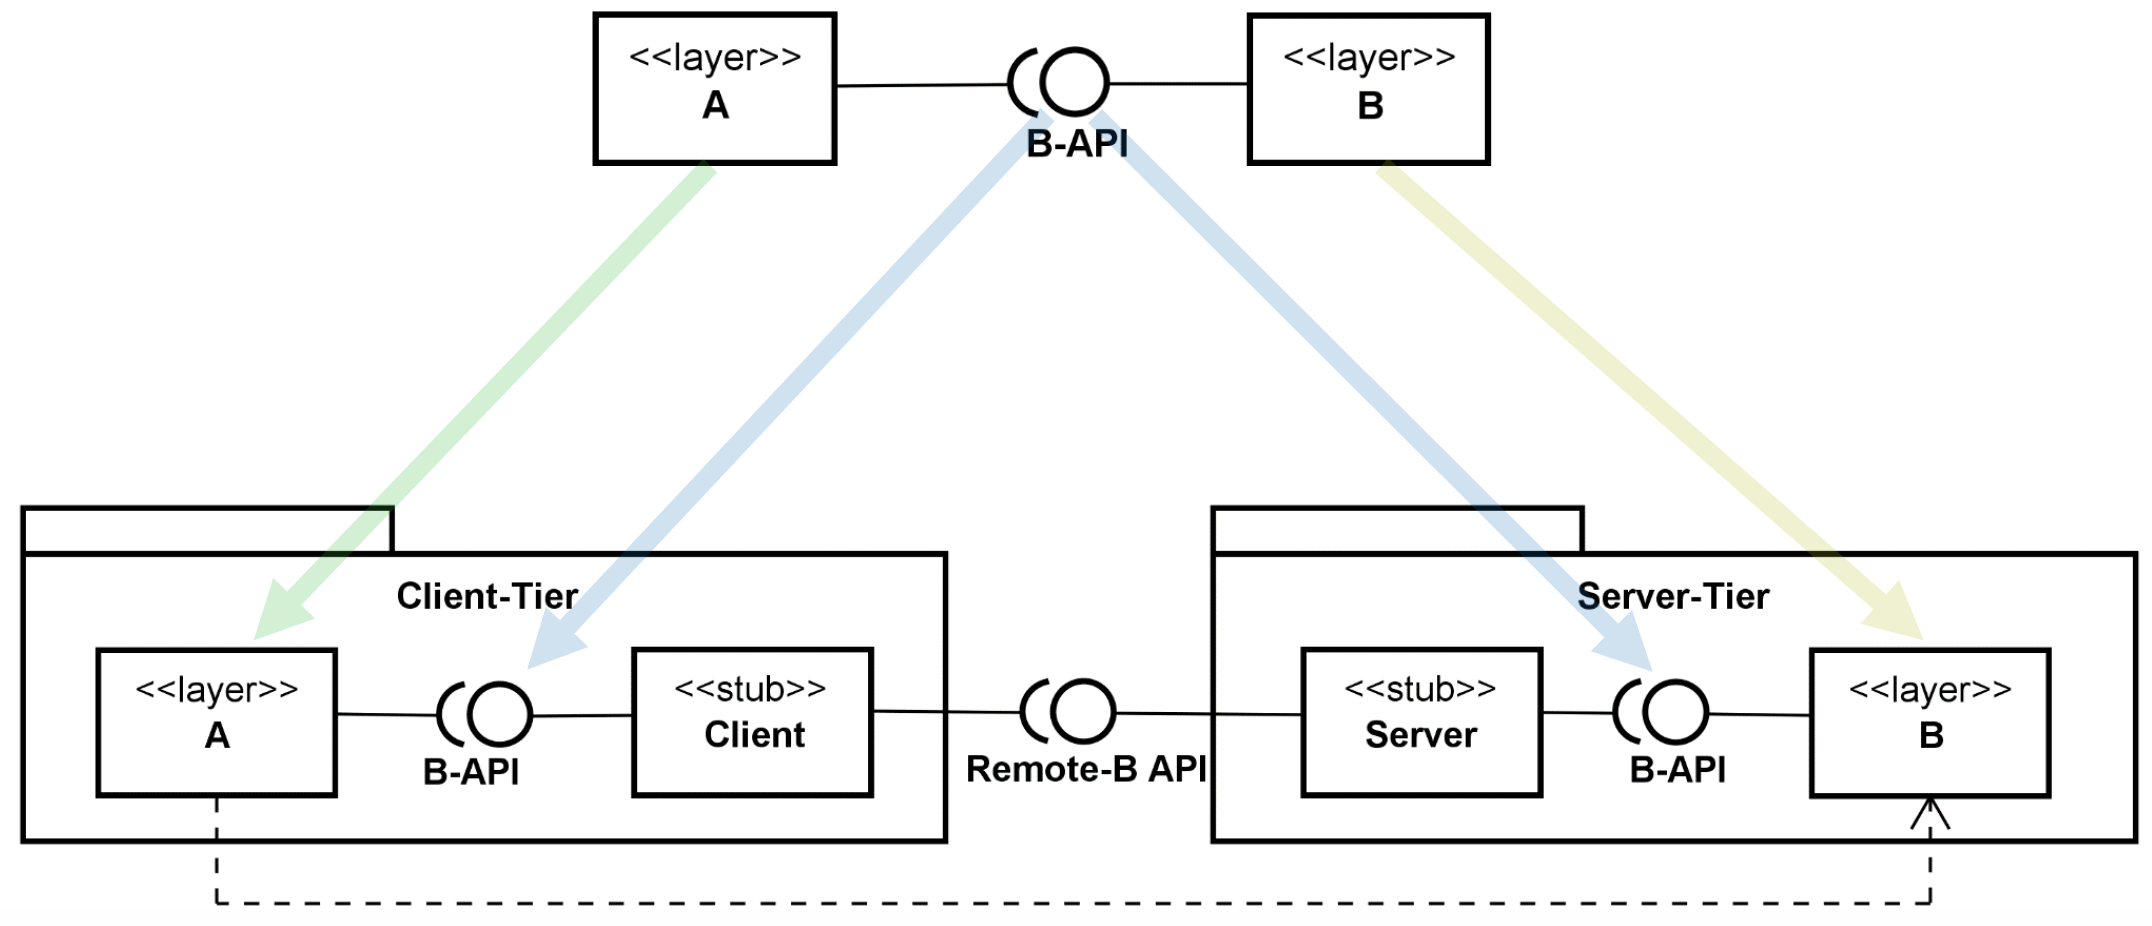
\includegraphics[keepaspectratio, height=5cm]{img/architecture/tiers.png}
						\caption{Aufteilung von Schichten auf Client / Server - Tiers}
						\label{fig:tiers}
					\end{figure}
			
			\newpage
			
			\subsubsection{Logische 3/6-Schicht-Architektur}
			
			Aufteilung in drei fundamentale Schichten:
			
			\begin{itemize}
				\item \textbf{Präsentation} (Presentation / [GU]I Layer):\\
						Visualisierung, User-Interface, Logik\\
						\textit{(bspw. Bestellmaske für Artikel)}
						
				\item \textbf{Geschäftslogik} (Business[logic] Layer, Domain Model):\\
						Implementation Geschäftsprozesse und -modelle\\
						\textit{(bspw. Ablauf einer Bestellung, Modell eines Artikels)}
						
				\item \textbf{Datenhaltung} {Data / Persistence Layer}\\
						Persistente Datenspeicherung, Datenlogik\\
						\textit{bspw. Speicherung der Artikeldaten in RDBMS}\\
						
				\item Diese Aufteilung lohnt sich quasi immer, unabhängig von physischer Verteilung\\
				$\rightarrow$ SoC (Separation of Concerns)\\
				$\rightarrow$ SRP (Single Responsibility Principle)\\
				$\rightarrow$ \textbf{Modularisierung!}				
			\end{itemize}
		
				\paragraph{Verfeinerung Präsentationsschicht}
				
					\begin{itemize}
						\item Reine Präsentation (Formulare, Dialoge etc.) bei Rich-GUI/Client:\\ 
						noch stärker von Präsentationslogik \& Daten trennen
						
						\item bspw. mit Model View Control (MVC):\\
						Modelle für Präsentation, wiederverwendbare Views, Präsentationslogik im Control
						
						\item Trennung zwingend notwendig bei Thin-Clients (bspw. Web/HTML):\\
						View durch HTML/CSS realisiert, Präsentationslogik und Modelle\\
						im Client (JS/JSON/XML) und im Server (Servlet, JSP, JSP/POJO's etc.)
					\end{itemize}
				
				\paragraph{Verfeinerung Geschäftslogikschicht}
				
					\begin{itemize}
						\item Businessfunktionen $\rightarrow$ \textbf{Services / Businessmethoden}\\
						Enthält Klassen für (Geschäfts-)Prozesse, arbeitet mit Domain Model\\
						(bspw. \texttt{BestellService} [Kunde bestellt Artikel])\\
						Kann technologisch weiter verfeinert werden bspw. Business Service als Web Service anbieten
						
						\item Business Objects, Domain Objects $\rightarrow$\textbf{Domain Model}\\
						Reines objektorientiertes Modell, vollständig unabhängig von Präsentation \& Persistenz, enthält Daten und Methoden (bspw. \texttt{Artikel}, \texttt{Kunde}, \texttt{Adresse})
					\end{itemize}
				
				\paragraph{Verfeinerung Datenhaltungsschicht}
				
					\begin{itemize}
						\item Trennung / Abstraktion der reinen Datenlogik:\\
						unabhängig vom physischen Datenmodell \& verwendetem (R)DBMS
						\item O/R-Mapping: Einsatz eines Persistenz-Frameworks
						\item Transparentes Einbinden von Legacy-Systemen, Abstraktion mehrerer Backend (DBMS-)Systeme
					\end{itemize}

				\begin{figure}[!htb]
					\centering
					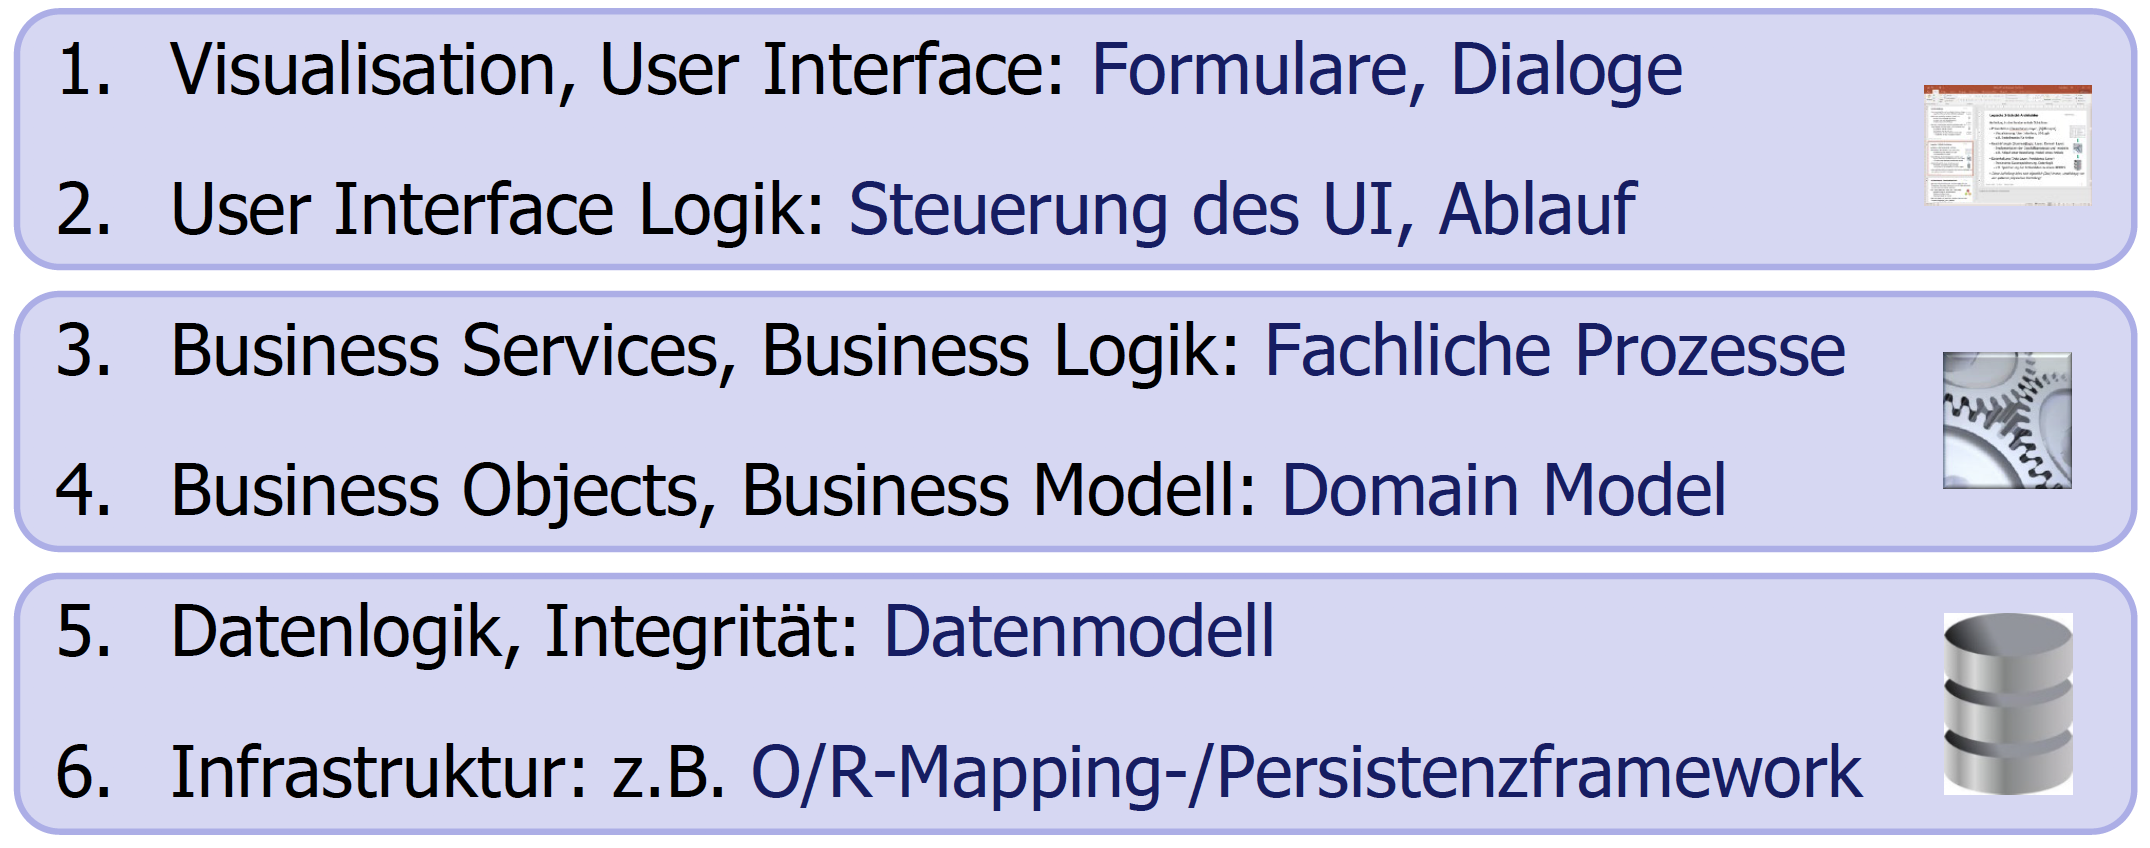
\includegraphics[keepaspectratio, height=5cm]{img/architecture/6layers.png}
					\caption{6-Schichten-Architektur aus Verfeinerung der 3-Schicht-Architektur}
					\label{fig:6layers}
				\end{figure}		
			
			\newpage
			
			\subsubsection{1, 2, 3, oder n-Schichten?}
			
			Je mehr Schichten ein System enthält...\\
			\textbf{Positive Effekte:}
			\begin{itemize}
				\item Bessere Strukturierung, einzelne Schichten kleiner und einfacher\\
				$\rightarrow$ besseres \& schnelleres Verständnis
				\item Grössere Chance auf Wiederverwendung
				\item Höhere Flexibilität bspw. Austausch einzelner Schichten
				\item Tendenziell bessere Skalierbarkeit
				\item Einfachere \& präzisere Planung / Schätzbarkeit
				\item Parallele \& getrennte Entwicklung möglich
			\end{itemize}
			\textbf{Negative Effekte:}
			\begin{itemize}
				\item Komplexität des Systems wird grösser
				\item Mehr Schnittstellen $\rightarrow$ mehr Aufwand $\rightarrow$ mehr Planung
			\end{itemize}
			
			
		\subsection{Sie sind sich der Bedeutung des Domänenmodells bewusst}

			\begin{itemize}
				\item Vollständige Abstraktion der Geschäftsprozesse und -daten\\
				'Reines' objektorientiertes Modell der Domäne, vollständige Trennung der physischen Datenspeicherung, Interaktion "nur" zwischen (Domain-)Objekten
				
				\item Logisches Beispiel: Klassen \texttt{Artikel} und \texttt{Lager}\\
				\texttt{Artikel}: Beschreibt konkreten Artikel, der einem Lagerort zugeordnet ist (entspricht Tupel)\\
				\texttt{Lager}: Beschreibt Lager, welches Artikel enthält, hat Fähigkeit Artikel zu reservieren, beziehen etc.
				
				\item Technische Beispiele:\\
				Enterprise Java Beans (Session \& Message Driven), \\
				Domain Model mit POJOs, übergeordnete Business-Services
			\end{itemize}
		
			\begin{figure}[!htb]
				\centering
				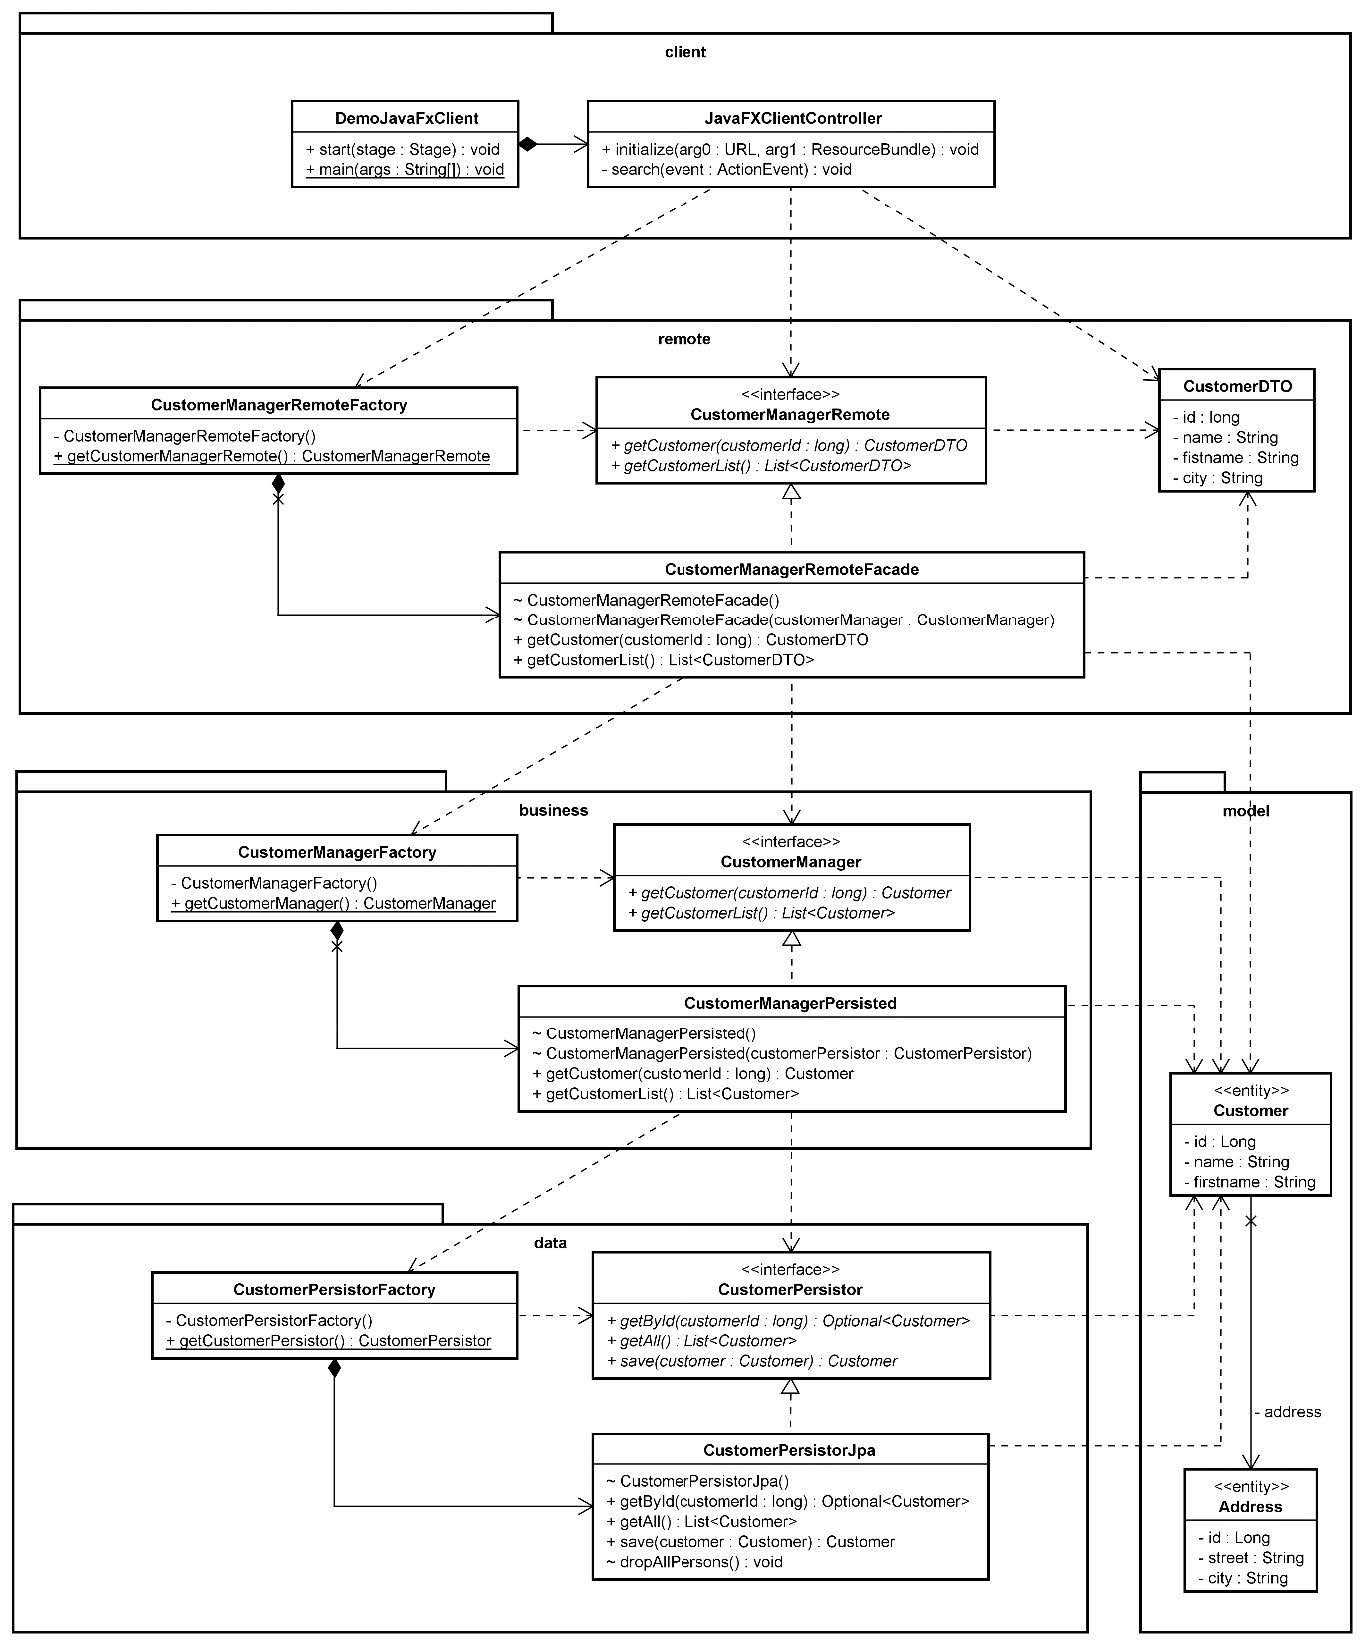
\includegraphics[keepaspectratio, height=12.6cm, angle=270, origin=c]{img/architecture/domainmodel.jpg}
				\caption{Einordnung des Domain Model in der Schichtenarchitektur}
			\end{figure}
		
			\newpage
			
			\paragraph{Domain Model - Diskussion}
			Realisiert praktisch alle Vorteile einer logischen 3-Schicht-Architektur, besonders:
			\begin{itemize}
				\item Entkopplung von Präsentation und Datenspeicherung
				\item Hohe Wiederverwendung (des Modelles)
				\item Gute Wart- und Erweiterbarkeit
				\item Starke Strukturierung, leichteres Verständnis
				\item Skaliert: auch für grosse / komplexe Enterprise-Systeme geeignet
			\end{itemize}
			Nachteile:
			\begin{itemize}
				\item Abstraktion / Mapping des Persistenzmodells verursacht Overhead (bspw. durch OR-Mapping)
				\item Effizienter Datenaustausch zw. Schichten ist herausfordernd \\
				(wiederholtes Mapping zur Entkopplung)
				\item \textit{Als Übung: Entwerfe ein Domänenmodell (fachliches Datenmodell) einer Anwendung, deren Funktion und Inhalt du gut kennst (gute Vorbereitung für Prüfungsaufgaben ;-) )} 
			\end{itemize}
		
			\paragraph{Schichtenarchitekturen - Bilanz}
			
			\begin{itemize}
				\item \textbf{Es kommt auf die Grösse an!}
				\item "Im Kleinen":\\
				Schichten funktionieren super und ergeben sich fast von selbst.\\
				Herausforderung: Ab wann ist Interface sinnvoll / nötig?, zu viele Schichten gibt es fast nicht, bspw. OSI-Schichtenmodell
				\item "Im Grossen":\\
				Schnittstellen sind Pflicht, was sich bspw. aus Aggregation aus Modulen fast selbst ergibt. Man tendiert hier eher zur Minimierung (so viel wie möglich)
				\item \textbf{Problem:} Nicht Anzahl ("Höhe") der Schichten ist die Herausforderung, sondern zu erkennen, wenn eine Schicht (oder ganzer Stack) zu breit wird.
				\item Domäne einer App wird evtl. zu gross, als Konsequenz werden Schichten zu breit und es sind Dinge darin zusammengelegt, die nichts mehr miteinander zu tun haben.\\
				Weiteres Mittel zur Partitionierung wird benötigt $\rightarrow$ \textit{Microservices?}
			\end{itemize}
		
		
		\subsection{Sie haben eine Vorstellung was Microservices sind}
		
		\begin{quote}
			\textit{“In short, the microservice architectural style is an approach to developing a single application as a suite of small services, each running in its own process and communicating with lightweight mechanisms, often an HTTP resource API. These services are built around business capabilities and independently deployable by fully automated deployment machinery.”\\
			- Martin Fowler}
		\end{quote}
		
		\begin{itemize}
			\item Eine Applikation wird in mehrere, kleine Services aufgeteilt
			\item Jeder Service läuft in eigenem Prozess / auf eigener Plattform
			\item Leichtgewichtige Kommunikation (meist RESTfull / HTTP / JSON)
			\item Voneinander unabhängig deploybar
			\item Automatisiertes Deployment (DevOps, PaaS, IaaS)
		\end{itemize}
	
				\paragraph{Aufteilung einer Applikation in kleine Services}
				
					\begin{itemize}
						\item Applikation (primär vertikal) in mehrere, (möglichst) eigenständige Teile aufteilen\\
								$\rightarrow$ Teile sollen autark arbeiten können \& auf eigene Daten(-modelle) zugreifen können
						\item Domänenmodell muss in verschiedene "bounded context" aufgebrochen werden\\
								$\rightarrow$ Gut für Design, aber nicht einfach, Datenhaltung ist so auch getrennt!
						\item Einzelne Teile sollten nicht (direkt) miteinander kommunizieren, werden über das GUI oder vorgelagerten Gateway orchestriert
						\item Microservices sind unterschiedlich gross, meistens gilt:\\
								Applikation > Microservice  $\geq$ Modul
					\end{itemize}
				
				\newpage
				
				\paragraph{Jeder Service hat eigenen Prozess / Plattform}
				
					\begin{itemize}
						\item Services als eigenständige Prozesse
							\begin{itemize}
								\item Unterschiedliche Plattformen (OS, Programmiersprach etc.), in virtualisiertem Container
								\item Plattformen für ganze App. müssen nicht identisch sein, können schrittweise geändert werden
							\end{itemize}
						\item Services laufen in echter Parallelität als verteiltes System
							\begin{itemize}
								\item Ganzes Potenziell, alle Herausforderungen von verteilten Systemen:\\
										$\rightarrow$ Netzwerkkommunikation, Latenz, Skalierung, Ausfall etc.
								\item Nutzt Client mehrere Services asynchron, erhöht sich Performance
							\end{itemize}
						\item \textbf{Komplexität des Systems erhöht sich!}
					\end{itemize}

				\paragraph{Leichtgewichtige Kommunikation}
				
					\begin{itemize}
						\item Populär: JSON-basierende REST-Schnittstellen (sind "einfach")
						\item Kritisch hinterfragen: JSON/REST "leichtgewichtig" im vergleich mit schnellen, effizienten binären Protokolle wie RMI, RPC etc.?
						\item Auf HTTP(S) basierende Kommunikation leicht zu implementieren \& automatisiert testbar\\
						$\rightarrow$ Authentifizierung \& Verschlüsselung abgedeckt, gute Akzeptanz im Operating, bestehende / bekannte Protokolle
					\end{itemize}
				
				\paragraph{Voneinander unabhängig deploybar / releasebar}
				
					\begin{itemize}
						\item Microservices: eigenständige Projekte / Releases, erst durch gemeinsame "Orchestrierung" eine Applikation $\rightarrow$ kleinere Einheiten flexibler entwickeln, Änderungen mit tieferem Risiko \& Erweiterungen leicht ergänzbar (OCP)
						\item Unabhängig deploybar: Gesamte Applikation damit umgehen können, dass einzelne Teile/Services ausfallen und nicht verfügbar sind
						\item Häufigere Ausfälle $\rightarrow$ Resilienz wird wichtig\\
						(Bei einem Teilausfall nicht vollständig versagen)
					\end{itemize}
				
				\paragraph{Deployment automatisiert (DevOps)}
				
					\begin{itemize}
						\item Automatisierung ist für Microservices ein Muss-Feature\\
								(mit schnelleren Start-/Stop-Sequenzen)
								
						\item Klassische, monolithische Deployments: (halb-)manuelle Deployments und Start-/Stop-Sequenz war häufig bei "schwergewichtigen" Applikationen $\rightarrow$ Manuell, fehleranfällig, Dauer im Bereich weniger Minuten, mit Microservices würde sich diese Tätigkeit um die Anzahl Microservices verlängern
					\end{itemize}
				
				\paragraph{Klassisch vs. Microservices}
				
					\begin{itemize}
						\item Schichten (horizontal) und Microservices (vertikal) sind orthogonal
						\item Am Schnittpunkt zwischen diesen befindet sich idealerweise ein Modul
						\item Entscheidend ist Grösse und Schnitt der Release- und Deployment-Einheiten
						\item Gegenseitige Abhängigkeiten sollen minimal sein
							\begin{itemize}
								\item Möglichst wenig und gering, ideal keine (minimale Kopplung)
								\item Microservices forcieren Modularisierung, verlagern das Problem ins Deployment (Operating)\\
							\end{itemize}
					\end{itemize}
				
				\textbf{Vorteile von Microservices:}
				\begin{itemize}
					\item einzeln überschaubar, unabhängig, gut wartbar
					\item relativ schnell \& flexibel (agil) anpassbar
					\item von kleinen, schlagkräftigen Teams entwickelbar
					\item unterschiedliche Plattformen, Sprachen \& Technologien
				\end{itemize}
				\textbf{Nachteile von Microservices:}
				\begin{itemize}
					\item Hohe Anfoderungen an Operatin (DevOps)
					\item Höhere Komplexität durch Asynchronität \& Resilienz
					\item Neue Herausforderung (cross-cutting concerns) wie \\
					Sicherheit, Überwachung, Monitoring \& Logging\\
				\end{itemize}
				\textbf{Herausforderung}: Design (bounded contexts) / verteilte Applikationen
					
		\newpage			
		
		\subsection{Sie kennen den Unterschied zwischen synchroner und asynchroner Kommunikation in verteilten Systemen}
		
		\begin{figure}[!htb]
			\centering
			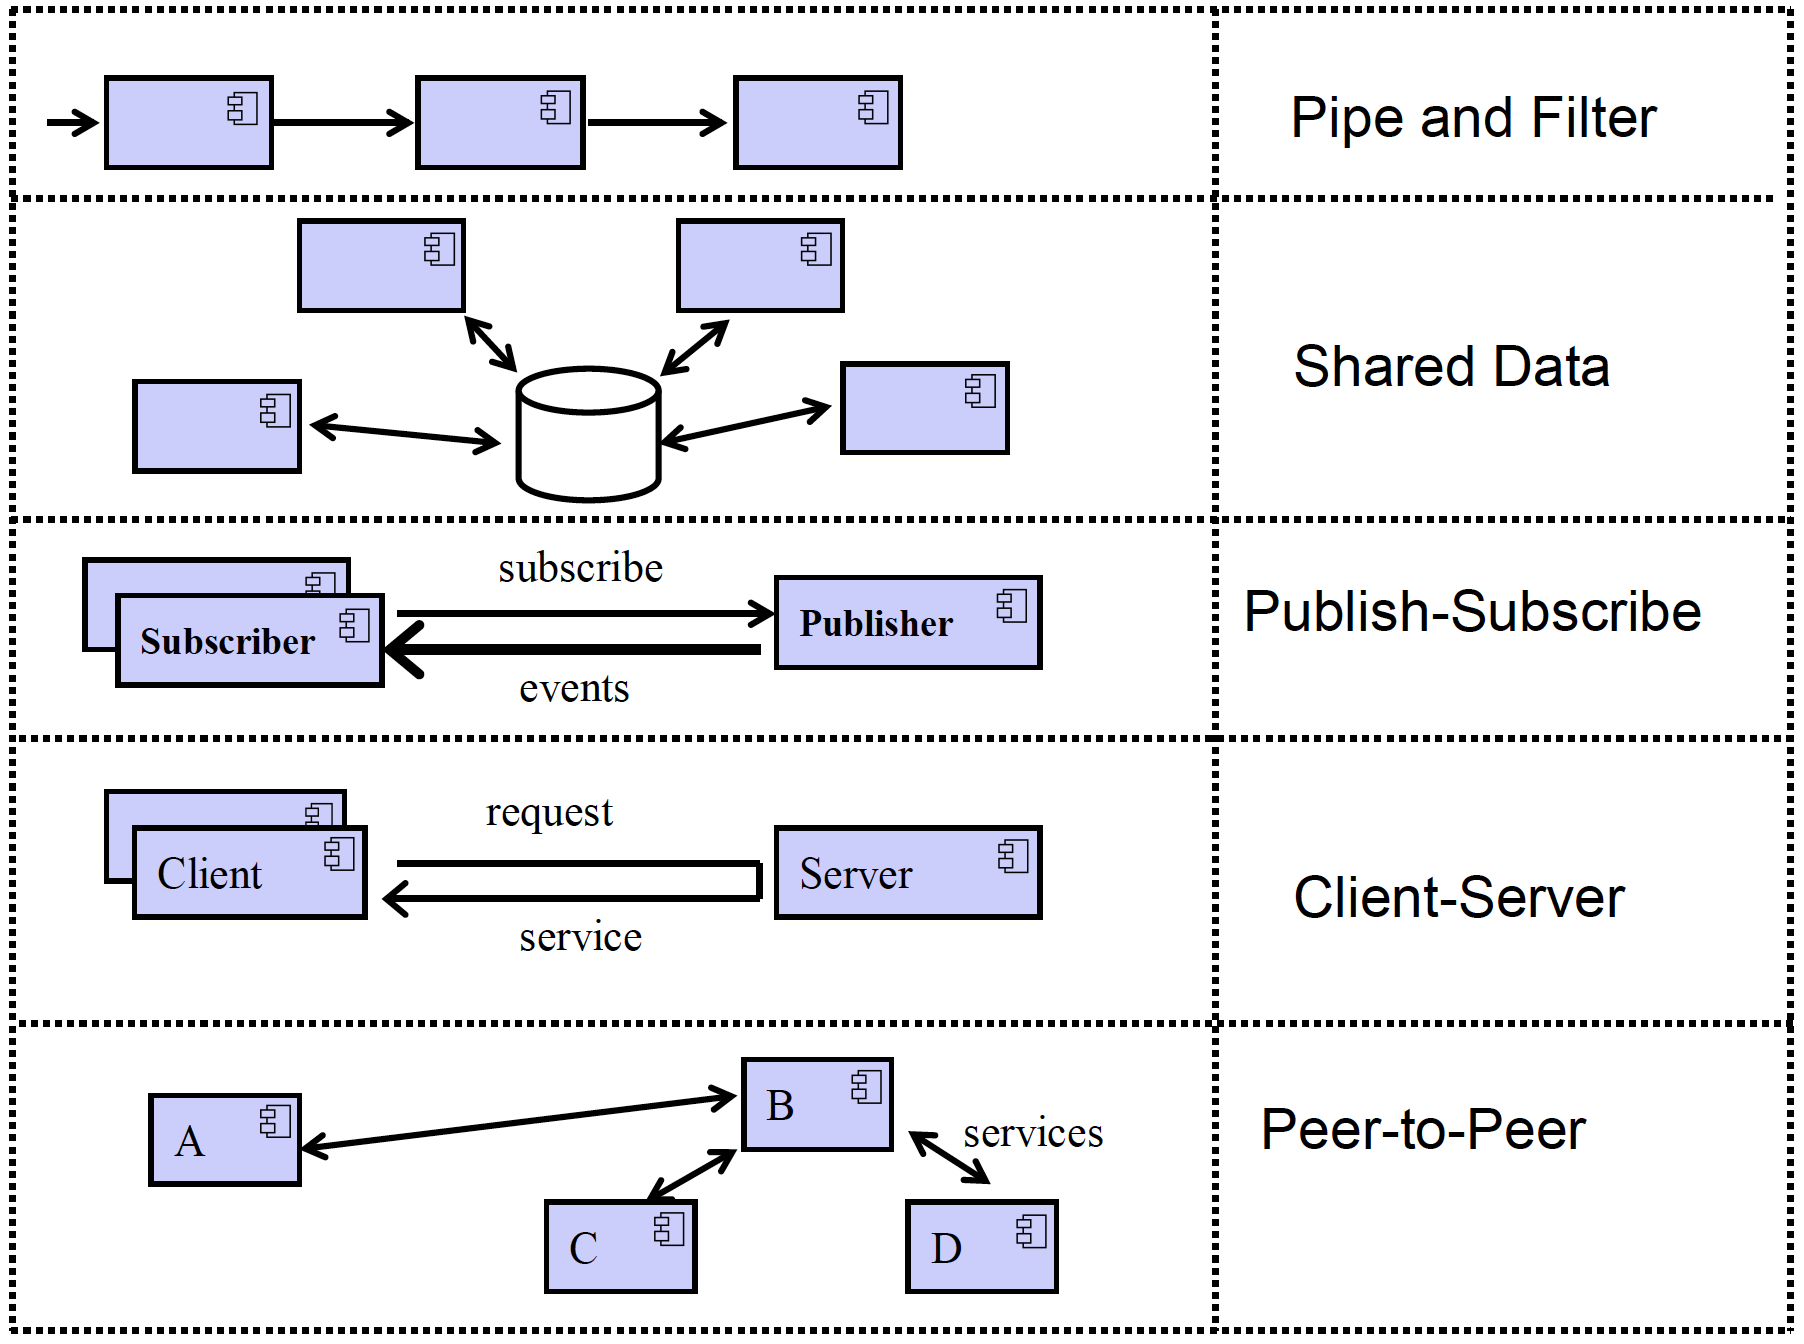
\includegraphics[keepaspectratio, height=6cm]{img/architecture/muster.png}
			\caption{Muster für verteilte Applikationen}
			\label{fig:muster}
		\end{figure}
	
		\begin{itemize}
			\item Einzelne Teile (Teilsysteme, Komponenten, Module, Services, Schichten etc.)\\
			auf mehrere versch. Rechner (hosts, tiers) verteilt
			\item Konsequenzen: Teile laufen in einzelnen unabhängigen Prozessen \& in "echter" Parallelität
			\item Anforderungen:
				\begin{itemize}
					\item Auswahl geeigneter Kommunikationstechnologie zw. Teilen
					\item Einzelne Teile müssen sich finden \& kenne
					\item Aufwändigeres Deployment, mehr und häufiger, Abhängigkeiten beachten \& koordinieren
					\item Mit Teilausfällen muss umgegangen werden können
				\end{itemize}
		\end{itemize}
	
	\newpage
	
	\subsubsection{Kommunikationsmodelle}
	
		\begin{figure}[htb!]
			\centering
			\begin{subfigure}{.45\textwidth}
				\centering
				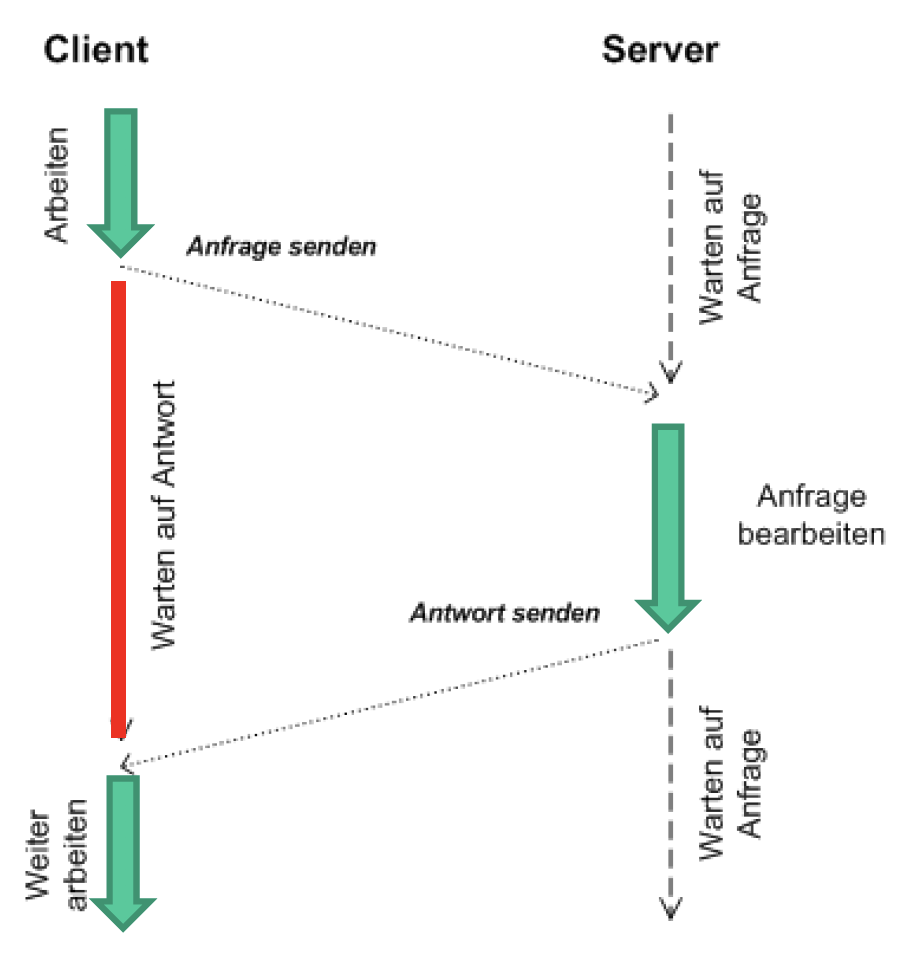
\includegraphics[keepaspectratio, height=6.5cm]{img/architecture/sync.png}
				\caption{Synchrone Kommunikation}
				\label{fig:synccomm}
			\end{subfigure}
			\begin{subfigure}{.45\textwidth}
				\centering
				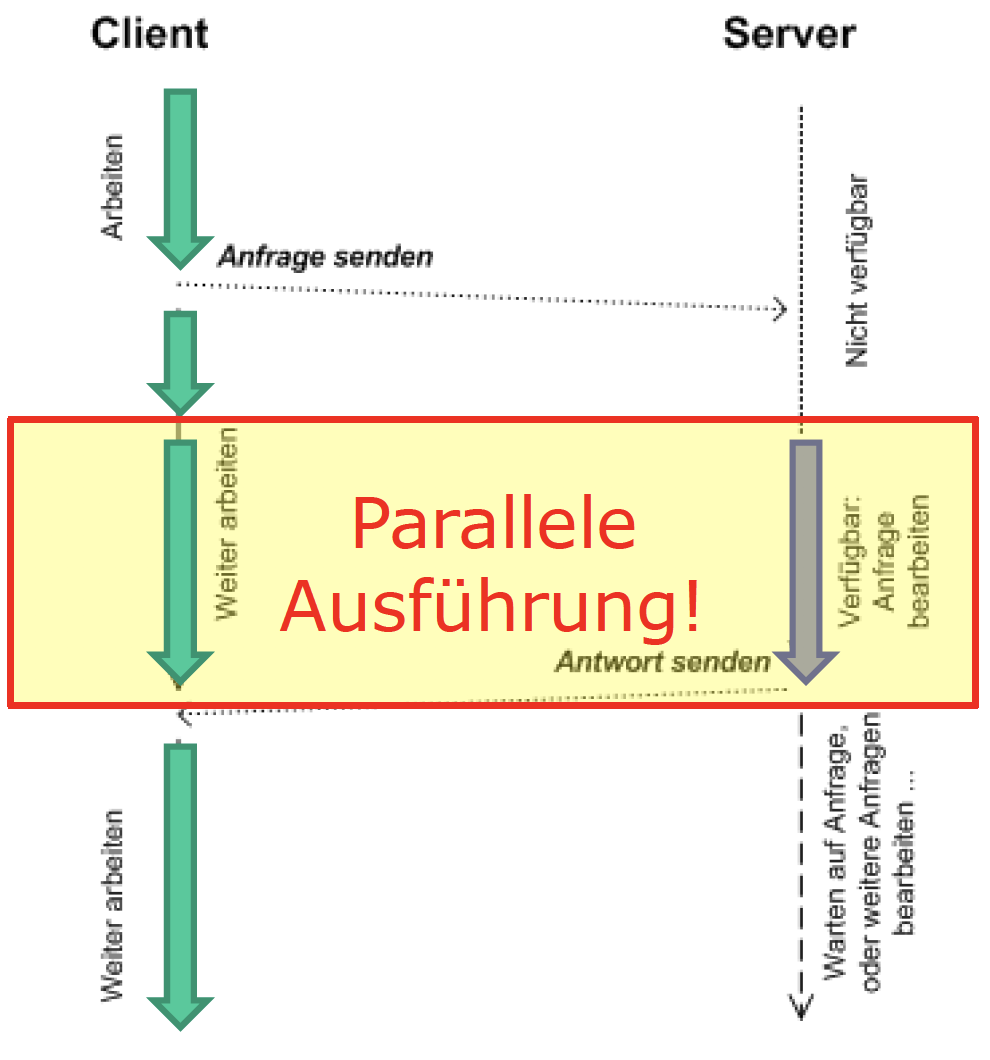
\includegraphics[keepaspectratio, height=6.5cm]{img/architecture/async.png}
				\caption{Asynchrone Kommunikation}
				\label{fig:asynccomm}
			\end{subfigure}
			\caption{Kommunikationsmodelle (synchron \& asynchron)}
			\label{fig:commmodels}
		\end{figure}

				\paragraph{Synchrones Modell / Kommunikation}
		
					\begin{itemize}
						\item Server muss verfügbar sein, bevor Kommunikation durch Client gestartet werden kann
						\item Sender muss auf Antwort des Empfängers warten, bevor er weiterarbeiten kann (blockierend)
					\end{itemize}
					\textbf{Vorteile:}
					\begin{itemize}
						\item Einfacher in Implementierung
						\item Zugriff auf gemeinsame Ressourcen weniger kritisch, da zeitlicher Ablauf überschaubar
					\end{itemize}
					\textbf{Nachteile:}
					\begin{itemize}
						\item "Wartezeit" beim Client: negative Auswirkung auf Performance (verlorene Zeit?)
						\item Enge Kopplung zw. Sender / Empfänger, weniger robust bspw. bei Ausfall
						\item Server muss verfügbar sein \& auf Anfragen warten
					\end{itemize}
			
				\paragraph{Asynchrones Modell / Kommunikation}
				
					\begin{itemize}
						\item Client kann Nachricht senden, egal ob Server für Empfang bereit oder nicht
						\item Client wird nicht blockiert, kann nach Übermittlung der Anfrage weiter arbeiten
						\item Antwort trifft später asynchron ein oder wird abgeholt
					\end{itemize}
					\textbf{Vorteile:}
					\begin{itemize}
						\item Lose Kopplung Client / Server $\rightarrow$ robuster
						\item Keine gegenseitige Blockierung \\
						(Server muss nicht Anfrage erwarten, Client muss nicht auf Antwort warten \& arbeitet weiter)
					\end{itemize}
					\textbf{Nachteile:}
					\begin{itemize}
						\item Komplexere Implementierung: zusätzliche Infrastruktur für Kommunikation (Queues)
						\item Wenn Client ohne Antwort nicht weiterarbeiten kann, macht async. Anfrage wenig Sinn
					\end{itemize}
				
	\newpage
	\section{Grafisches User Interface - mit JavaFX}	
		
		\subsection{Sie wissen, was unter deklarative GUI Beschreibung zu verstehen ist und welche Vorteile dieses Vorgehen mit sich bringt}
		
		\begin{itemize}
			\item JavaFX im Code erstellen: \\
			Komponenten erstellen, verknüpfen und Verhalten ad hoc vor Ort implementieren
			\item JavaFX GUI in FXML (JavaFX Markup Language) deklarativ beschreiben \\
			nach \textbf{Model View Control} Pattern:
				\begin{itemize}
					\item GUI-Komponenten (View) werden mithilfe von FXML beschrieben
					\item Verhalten (Controller) und Datenmodell (Model) mit Java-Klassen implementieren
				\end{itemize}
			\item Ermöglicht Trennung zw. Modell / Verhalten und der Darstellung
			\item Schnellere GUI-Erstellung (GUI-Code in XML-Datei)
			\item Bessere Code-Wartbarkeit
			\item GUI-Erstellung kann von Designer, Verhalten von Programmierer übernommen werden
			\item Einfachere Anpassung unterschiedlicher Ausgabetypen (Desktop, Tablet, Handy)\\
			$\rightarrow$ gerätespezifische FXML-Datei
		\end{itemize}
		
		\subsection{Sie sind in der Lage ein einfaches GUI mit Hilfe von SceneBuilder zu erstellen und in die Applikation korrekt zu integrieren}
		
		\textit{(Nei ned werkli, aber ech Kopy-Pasta mol d Biispel \& Demo us de Folie)}
		
		\begin{figure}[!htb]
			\centering
			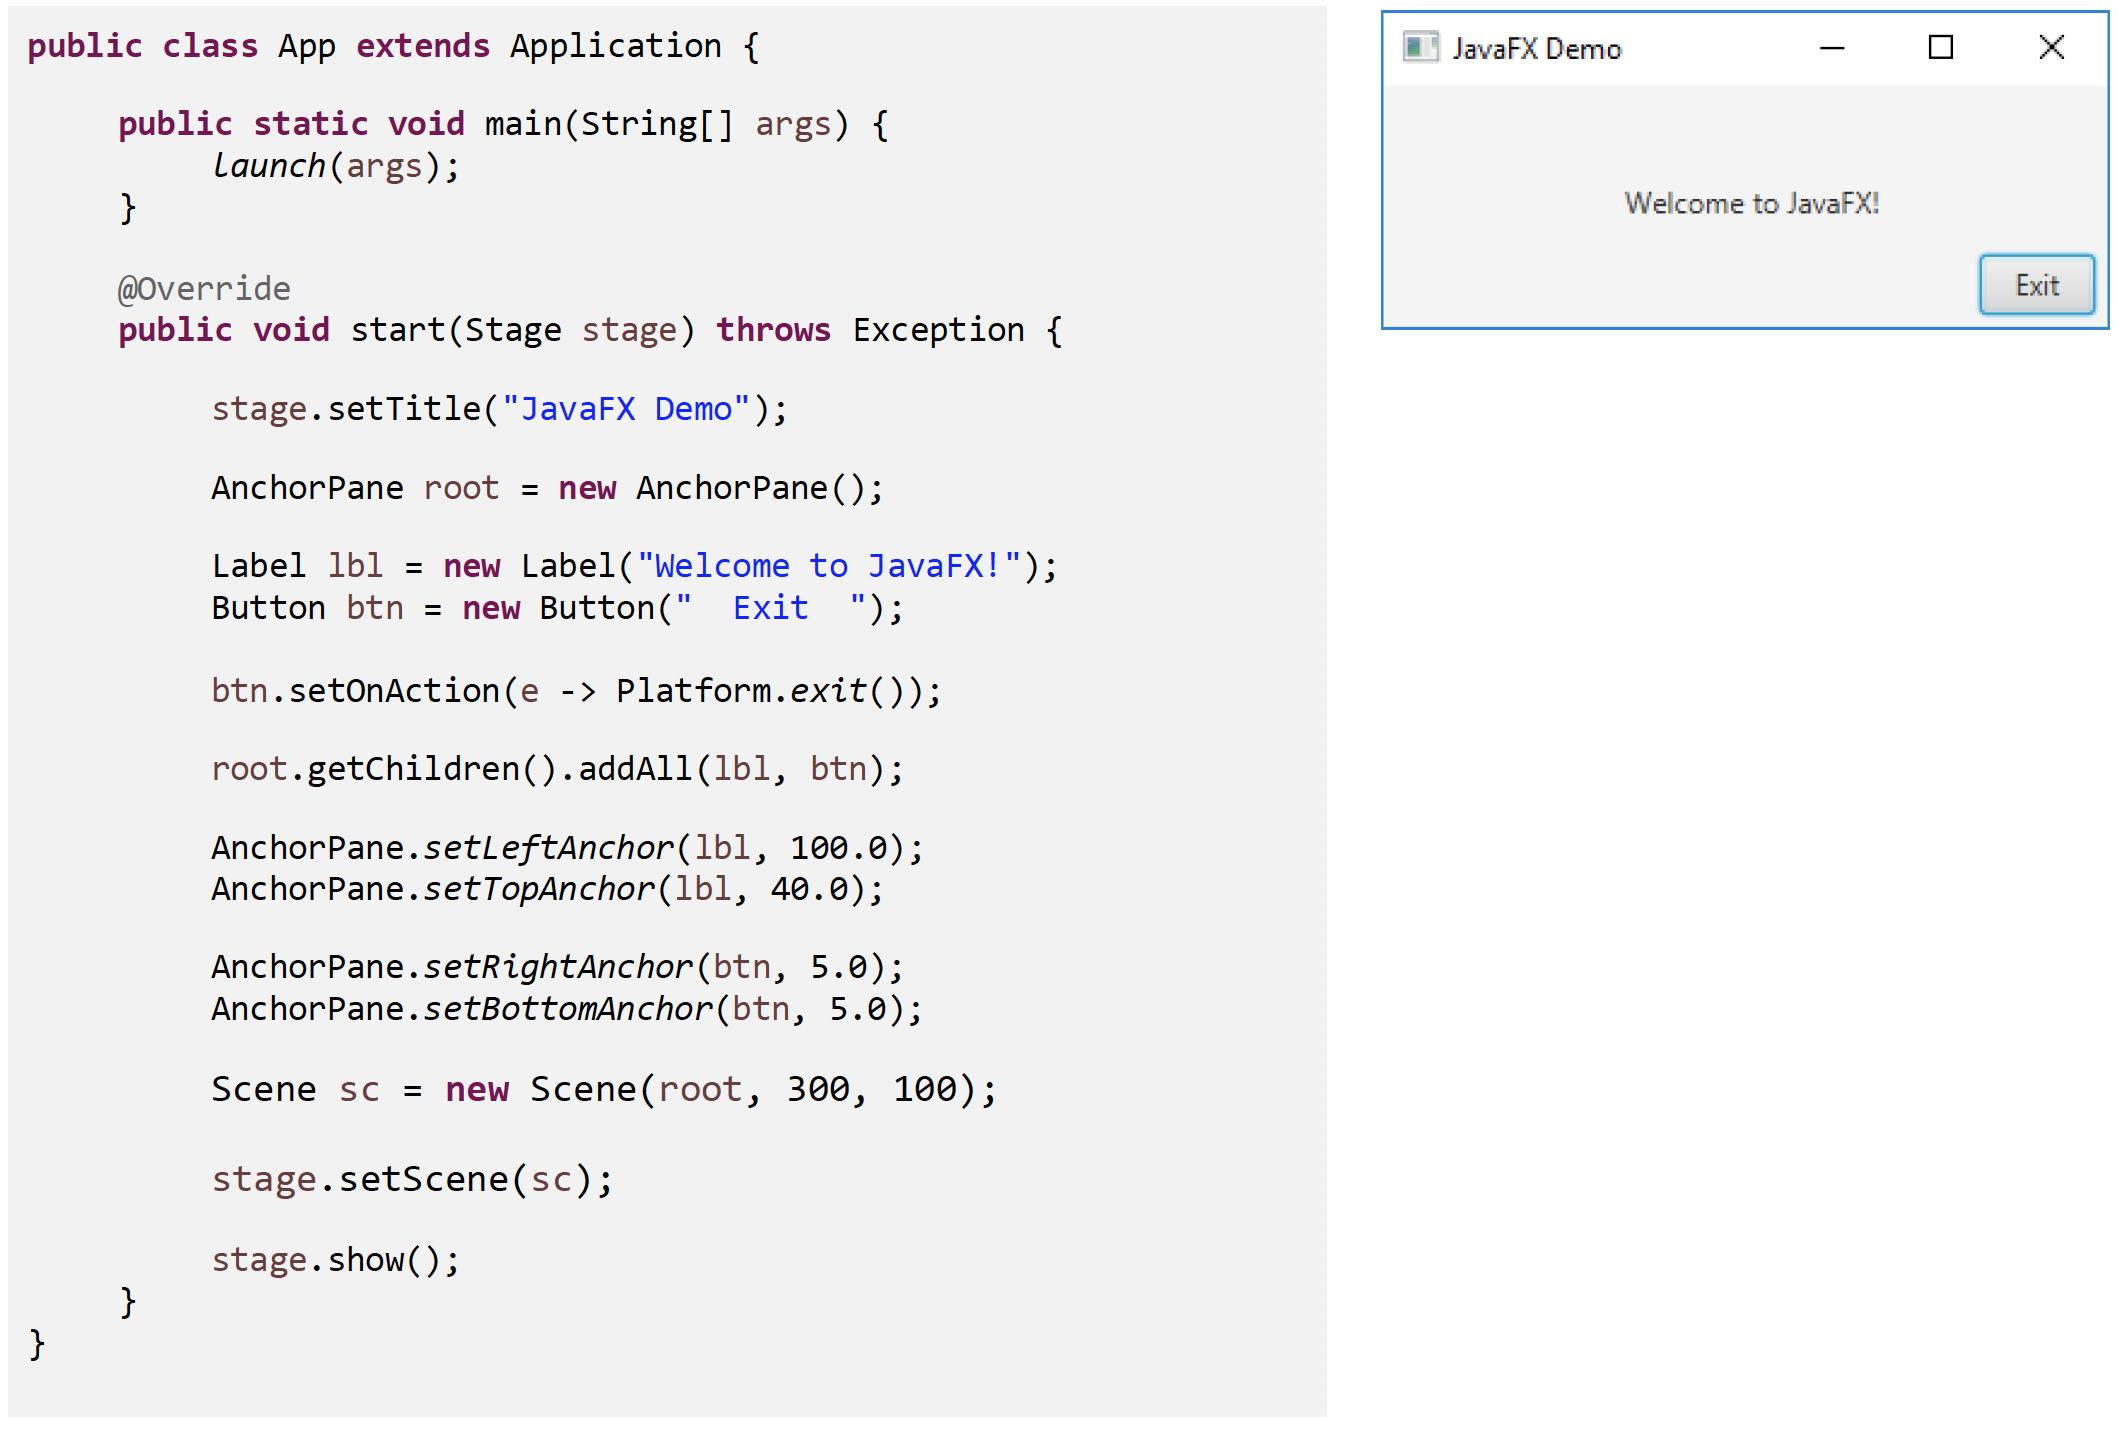
\includegraphics[keepaspectratio, width=\textwidth]{img/gui/gui.png}
			\caption{Traditionelle GUI-Programmierung}
			\label{fig:tradgui}
		\end{figure}
		
		\newpage
		\noindent
		\textbf{Aufgabe}: JavaFX-App, welche prüfen soll, ob eingegebene Zahl eine Primzahl ist. 
		GUI-Aufbau deklarativ mit FXML. 
		Für Erstellung der FXML-Datei soll SceneBuilder verwendet werden.
		
		\begin{figure}[!htb]
			\centering
			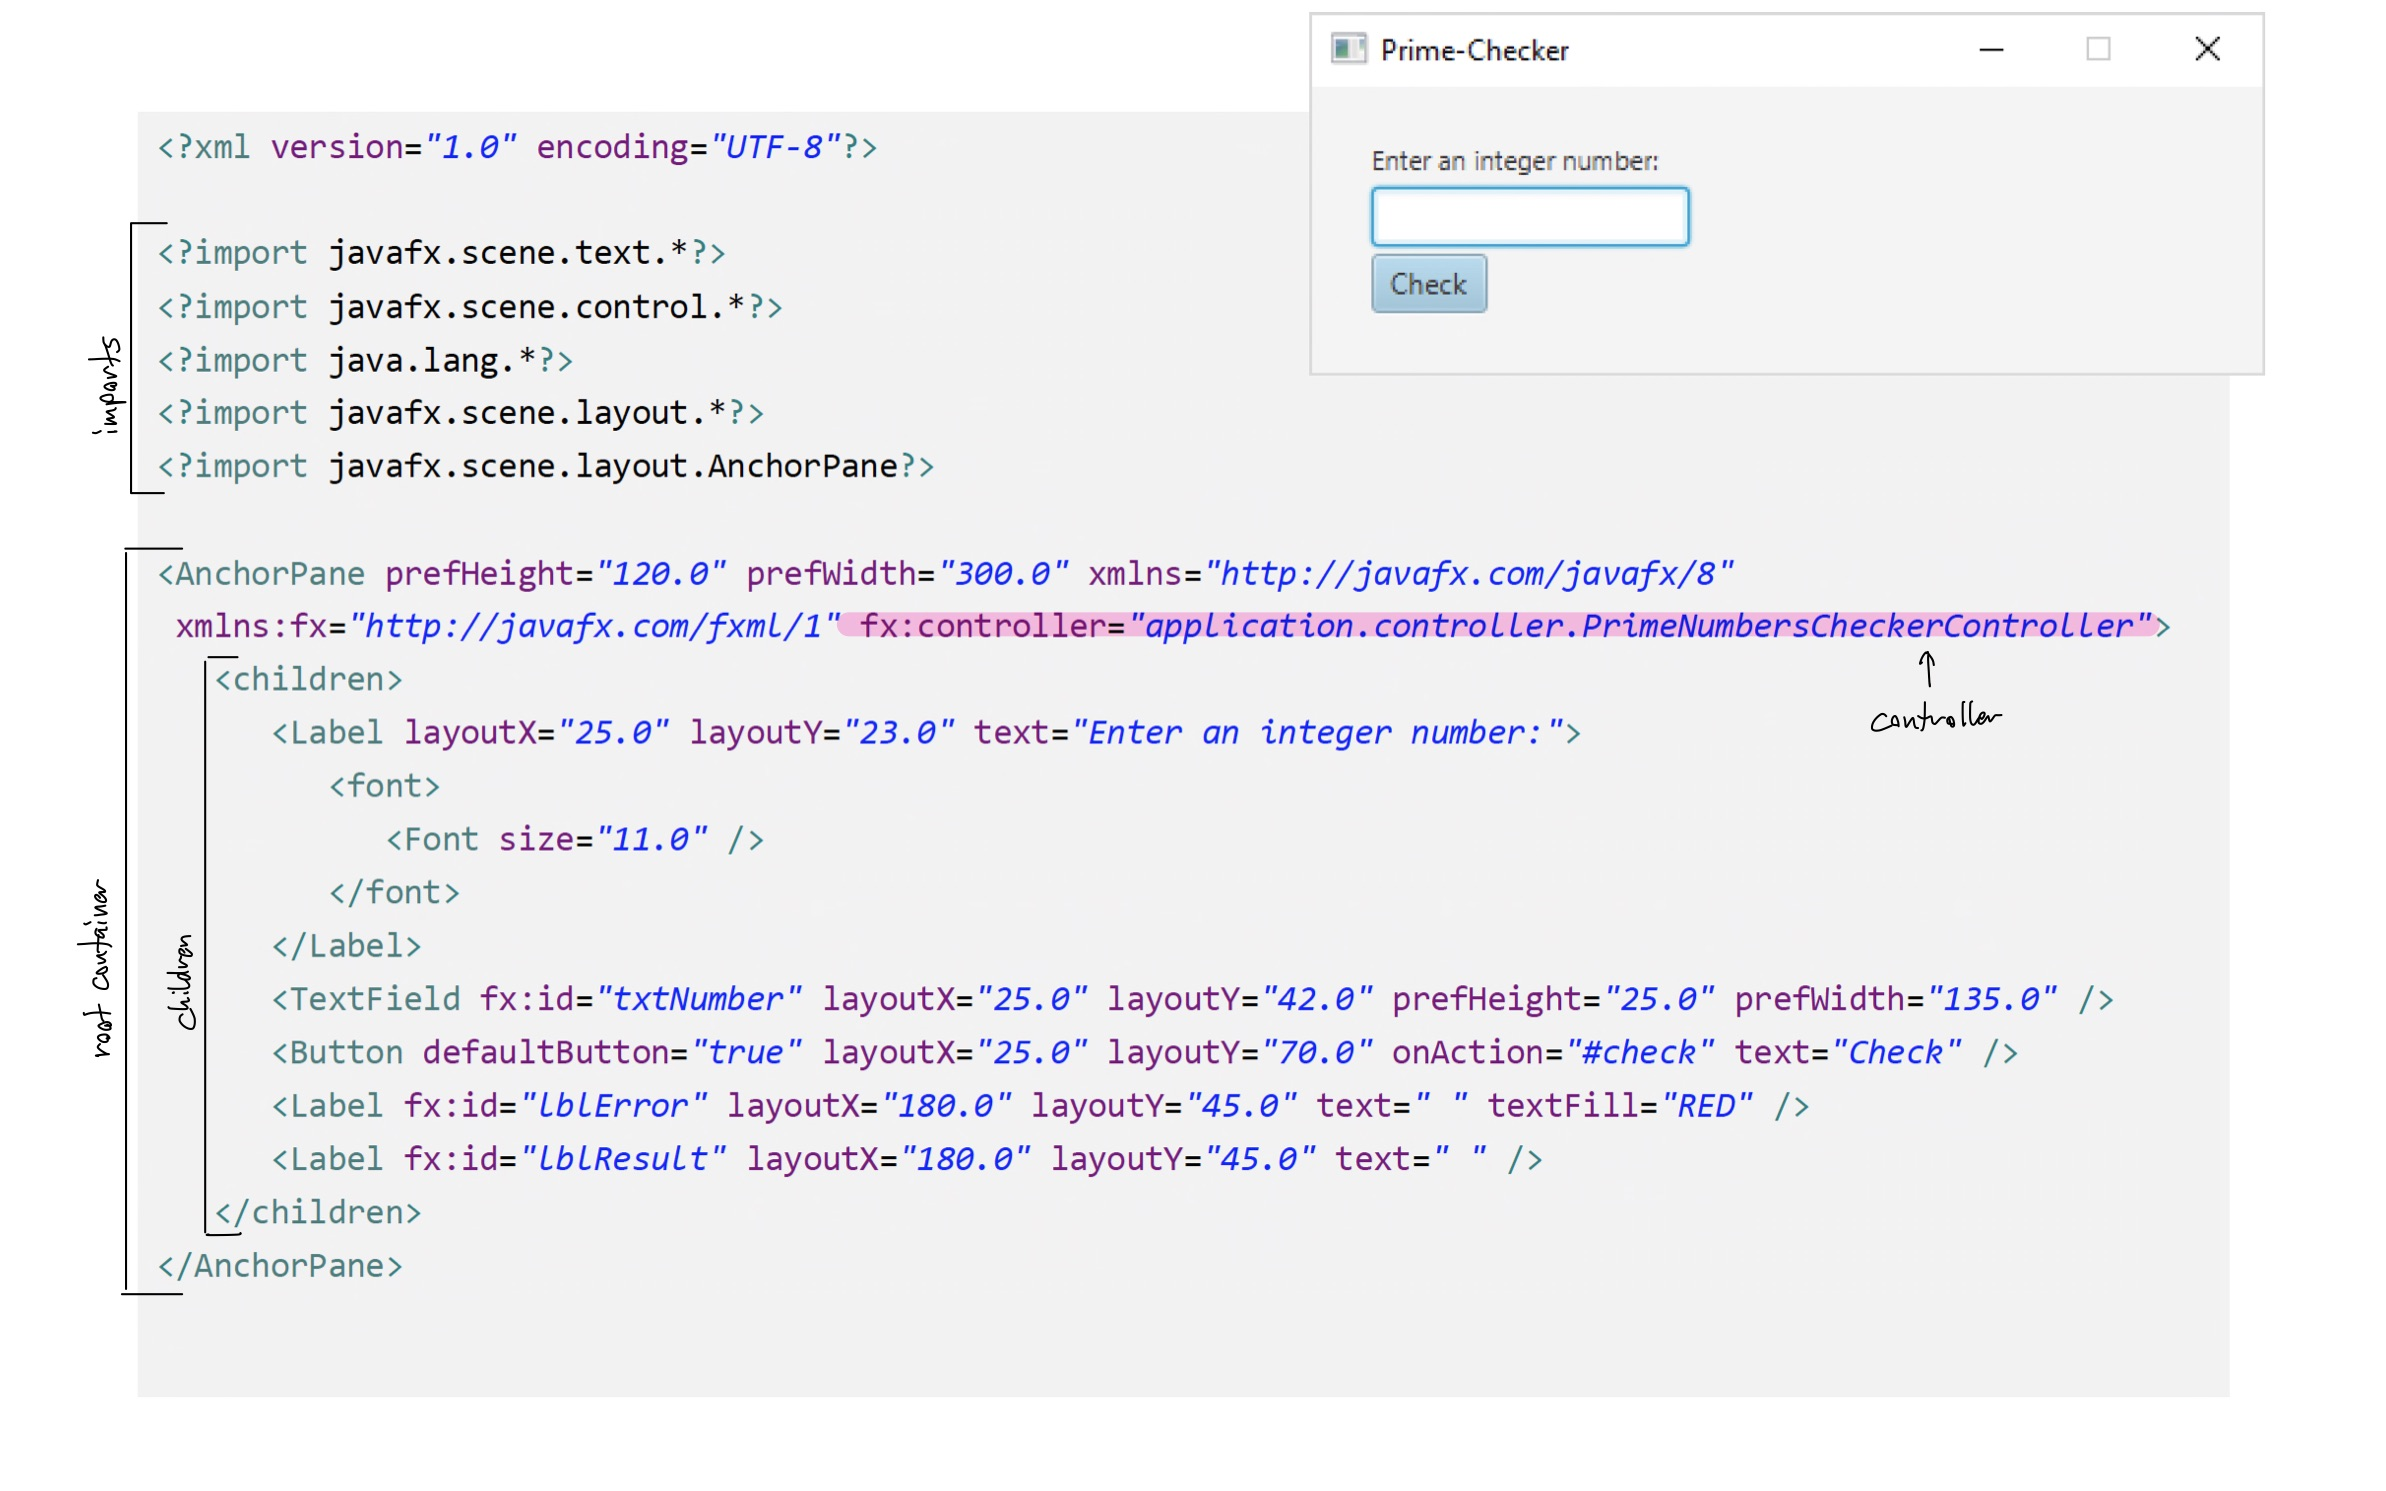
\includegraphics[keepaspectratio, width=\textwidth]{img/gui/fxml.jpg}
			\caption{FXML-Datei für ein GUI}
			\label{fig:fxmlgui}
		\end{figure}
		\textbf{FXML-Datei laden}
		\begin{itemize}
			\item GUI-Aufbau Implementierung im Code entfällt dank XML-Deklaration
			\item GUI mithilfe der \texttt{FXMLLoader}-Klasse erstellen:\\
			FXML-Datei mithilfe von \texttt{load()} im Code laden
		\end{itemize}
		\noindent
		\textbf{Beispiele} (versch. Variante, Code in der Klasse \texttt{application.}App)
		
		\begin{lstlisting}
AnchorPane root = FXMLLoader.load(getClass()
	.getResource("view/PrimeNumberCheckerView.fxml");
	
AnchorPane root = FXMLLoader.load(getClass()
.getResource("application/view/PrimeNumberCheckerView.fxml");

AnchorPane root = FXMLLoader.load(getClass().getClassLoader()
.getResource("application/view/PrimeNumberCheckerView.fxml");
		\end{lstlisting}
		\noindent
		FXML-Datei sinnvollerweise in Unterpaket ablegen (bspw. \texttt{view}), Laden der ersten FXML-Datei in der Methode \texttt{start}:
		
		\begin{figure}[!htb]
			\centering
			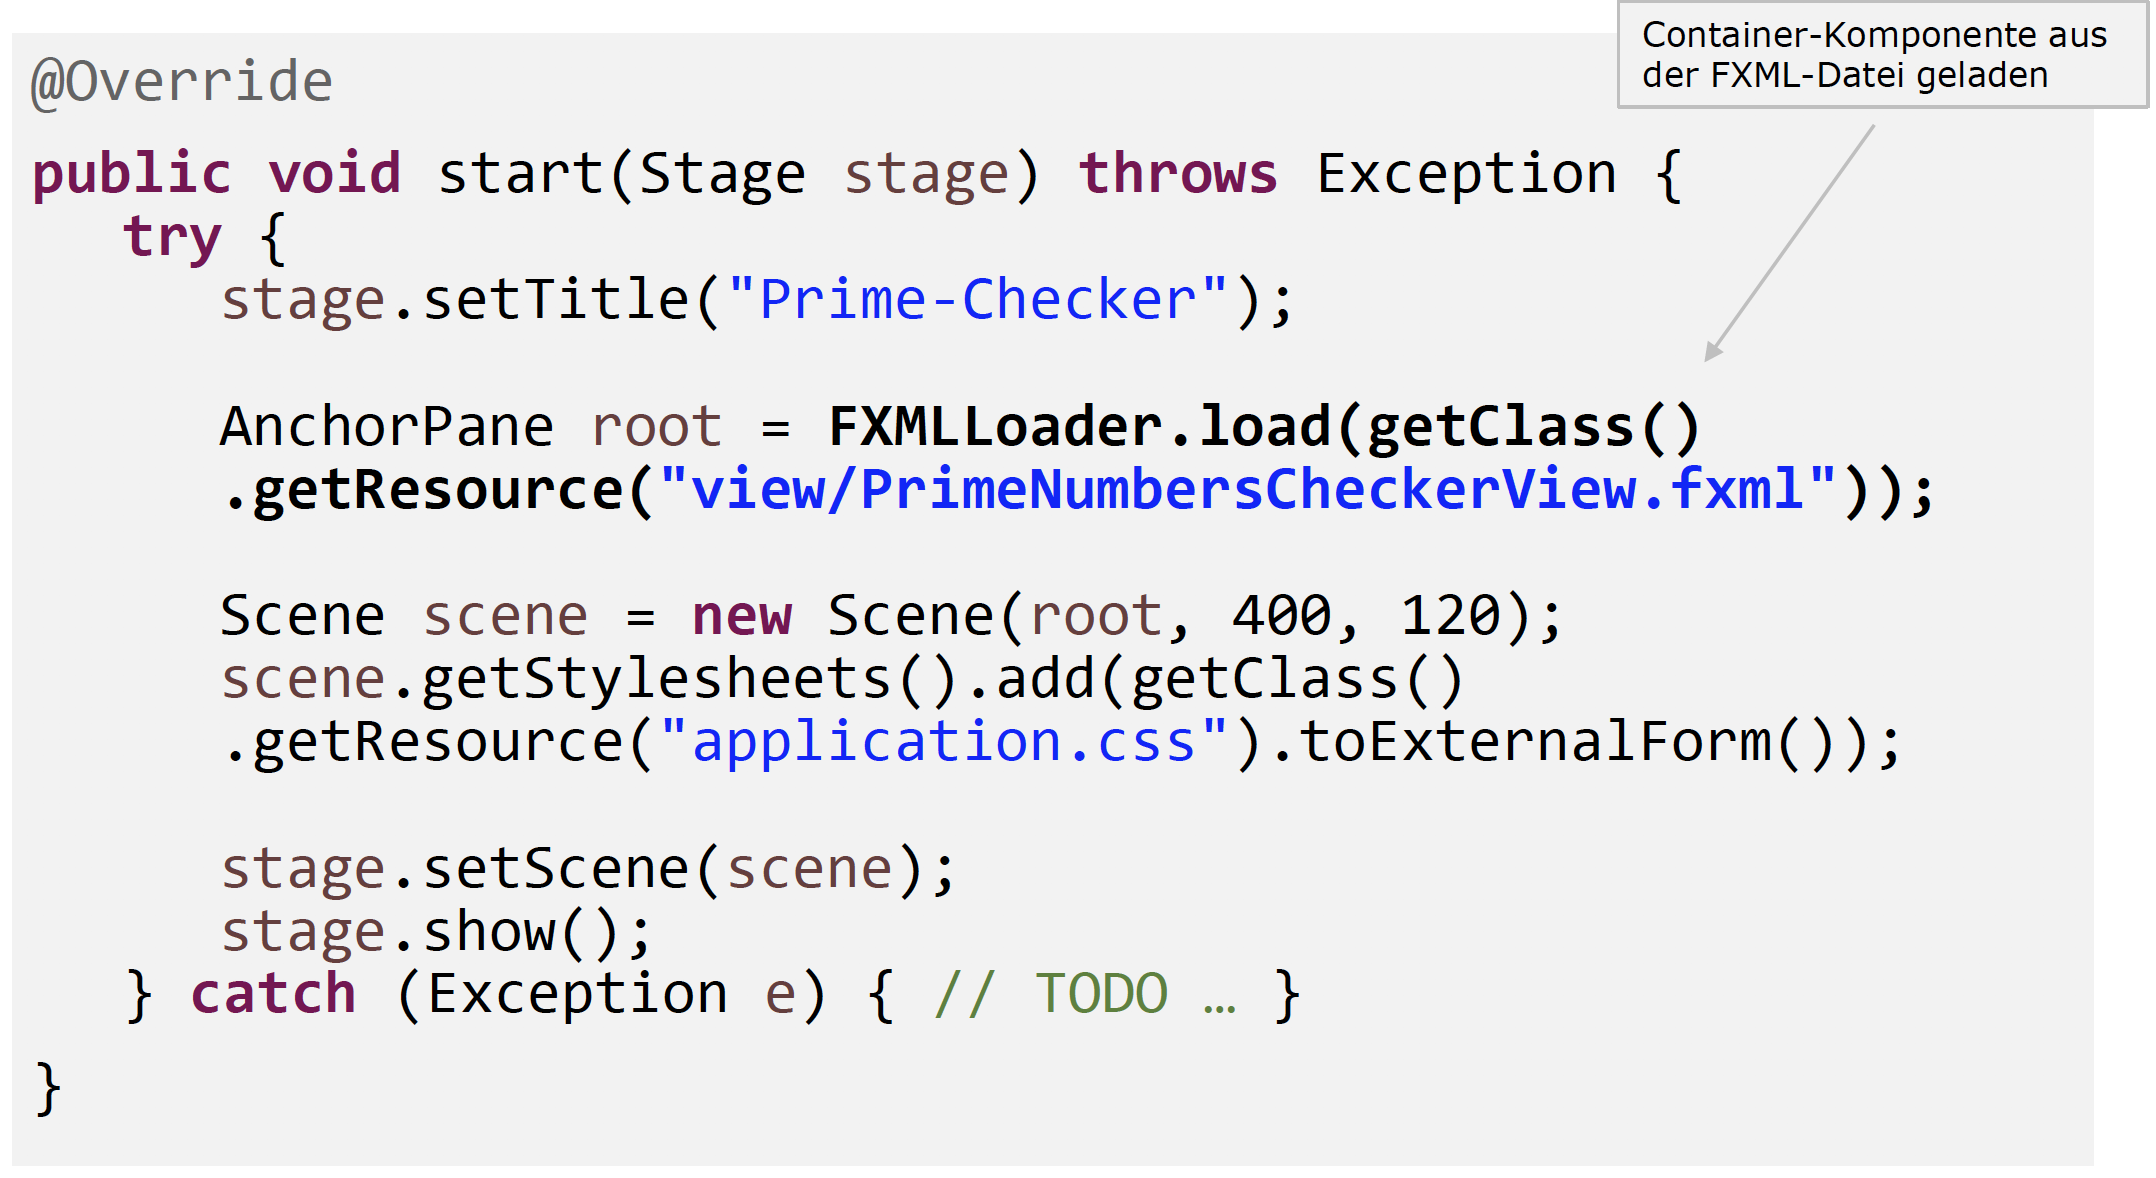
\includegraphics[keepaspectratio, height=4cm]{img/gui/start.png}
			\caption{Implementierung in der \texttt{start}-Methode}
			\label{fig:startimpl}
		\end{figure}
		
		\newpage
		
		\paragraph{Verhalten implementieren}
		
		\begin{itemize}
			\item GUI-Komponenten (Buttons, Textfelder, Radio-Button, Menu-Item etc.):\\
			Lösen Aktionen aus, sind in Controller-Klasse in Form von Methoden implementiert
			\item Controller-Klasse:\\
			Notwendig, auf GUI-Komponenten zuzugreifen, welche aber in FXML-Datei definiert wurden
			\item \textbf{Lösung}: Komponenten beim Laden des FXML durch Injection dem Controller zur Verfügung stellen\\
			$\rightarrow$ @FXML Annotation
		\end{itemize}
	
		\begin{figure}[!htb]
			\centering
			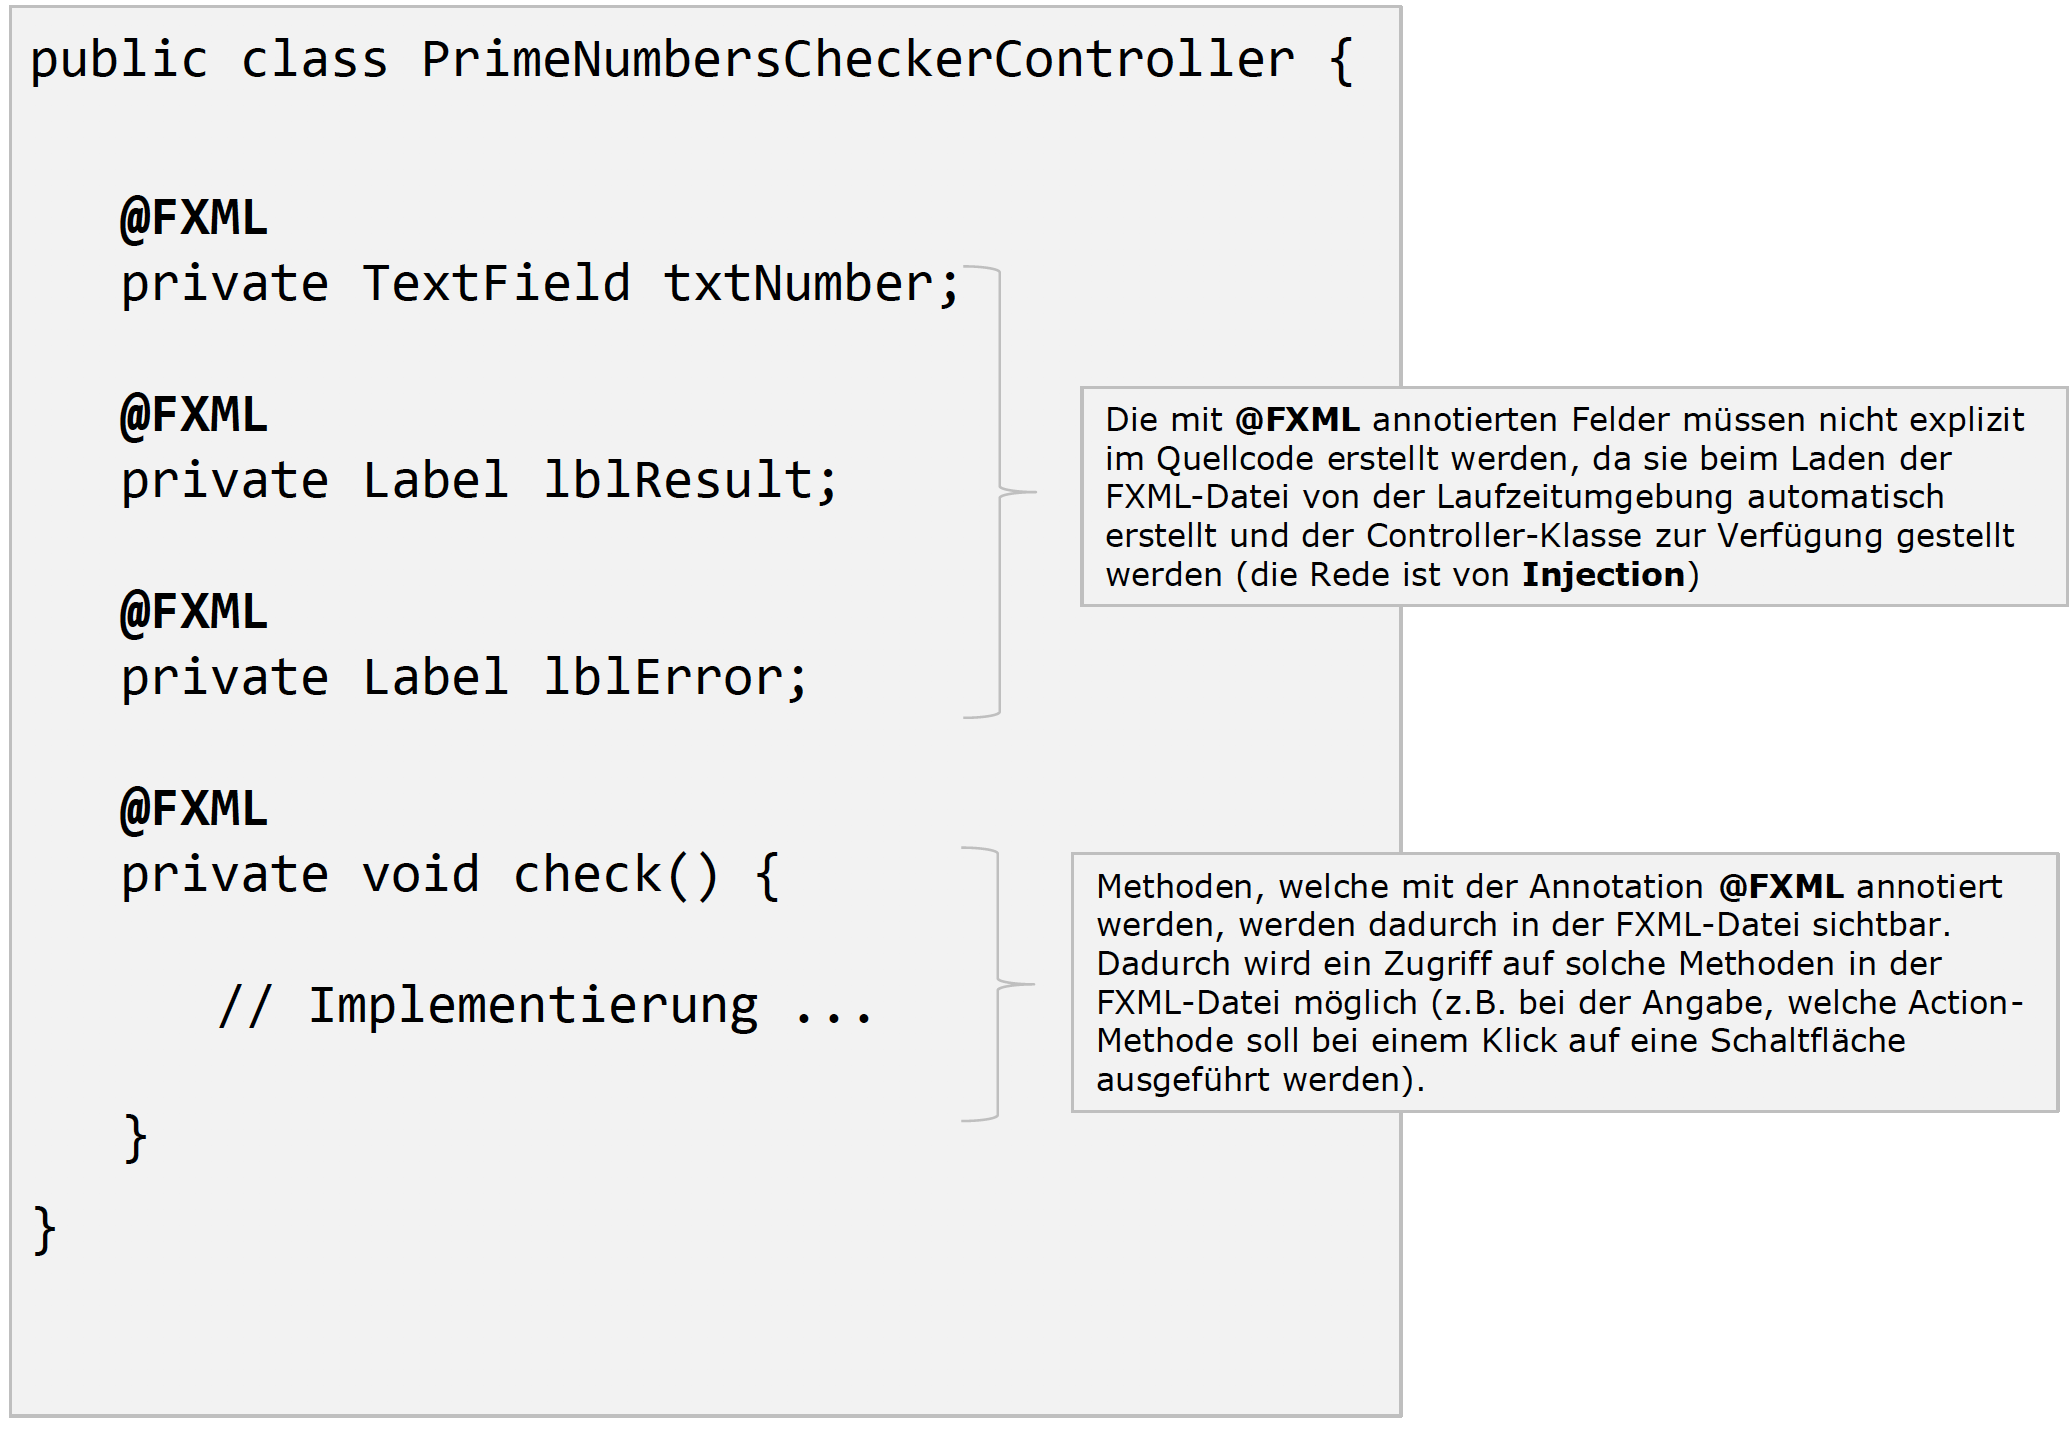
\includegraphics[keepaspectratio, height=8cm]{img/gui/verhalten.png}
			\caption{Implementierung des Verhaltens im Controller}
			\label{fig:verhalten}
		\end{figure}
		
		\subsubsection{JavaFX mit SceneBuilder}
		
		\begin{figure}[!htb]
			\centering
			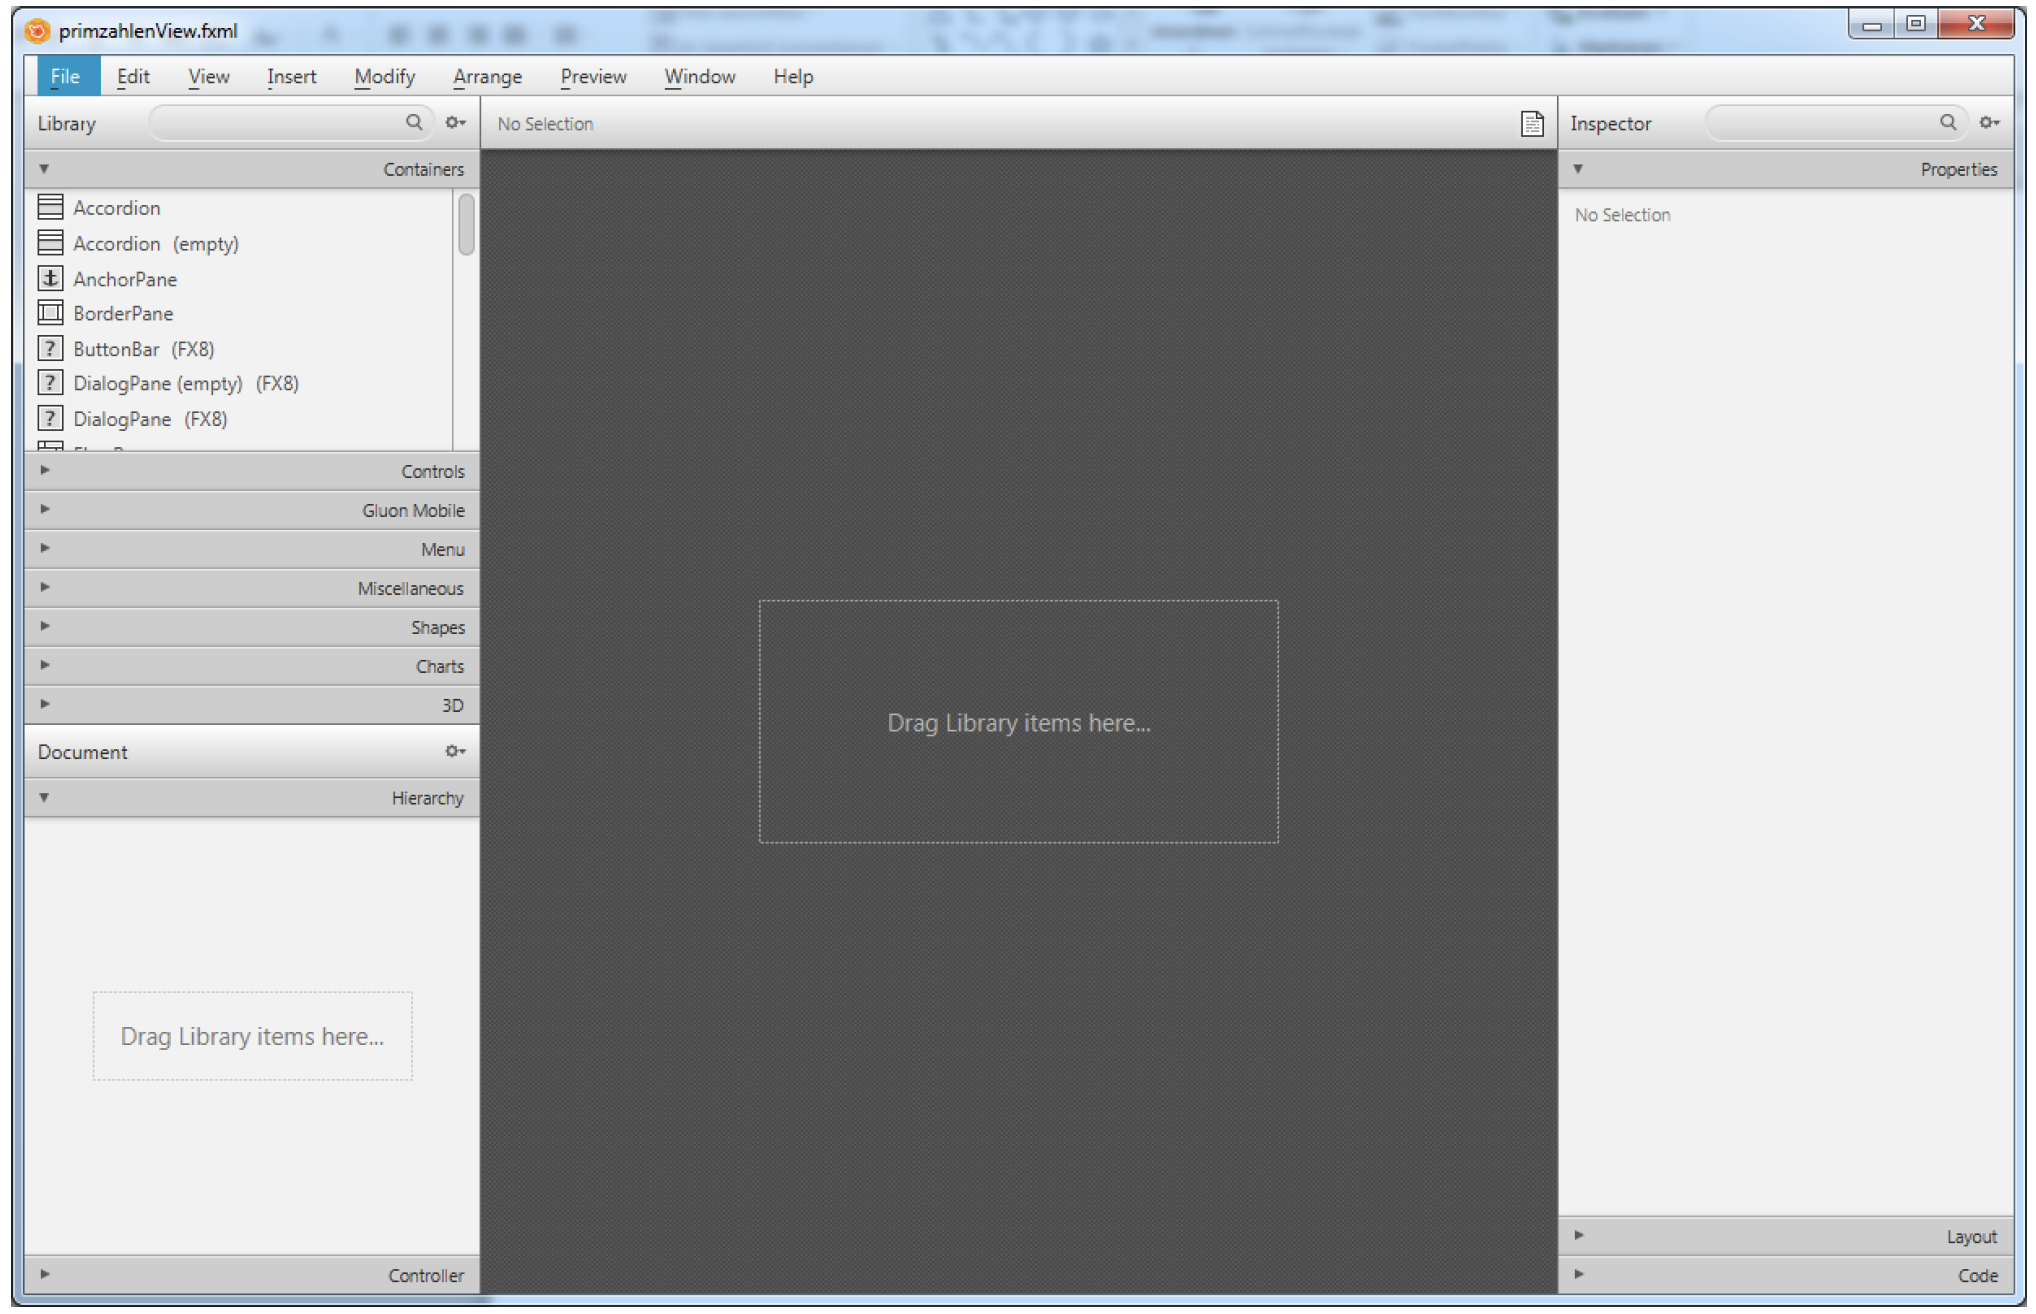
\includegraphics[keepaspectratio, height=7cm]{img/gui/scenebuilder.png}
			\caption{Ansicht des SceneBuilder}
			\label{fig:scene01}
		\end{figure}
	
		\newpage
	
		\begin{figure}[!htb]
			\centering
			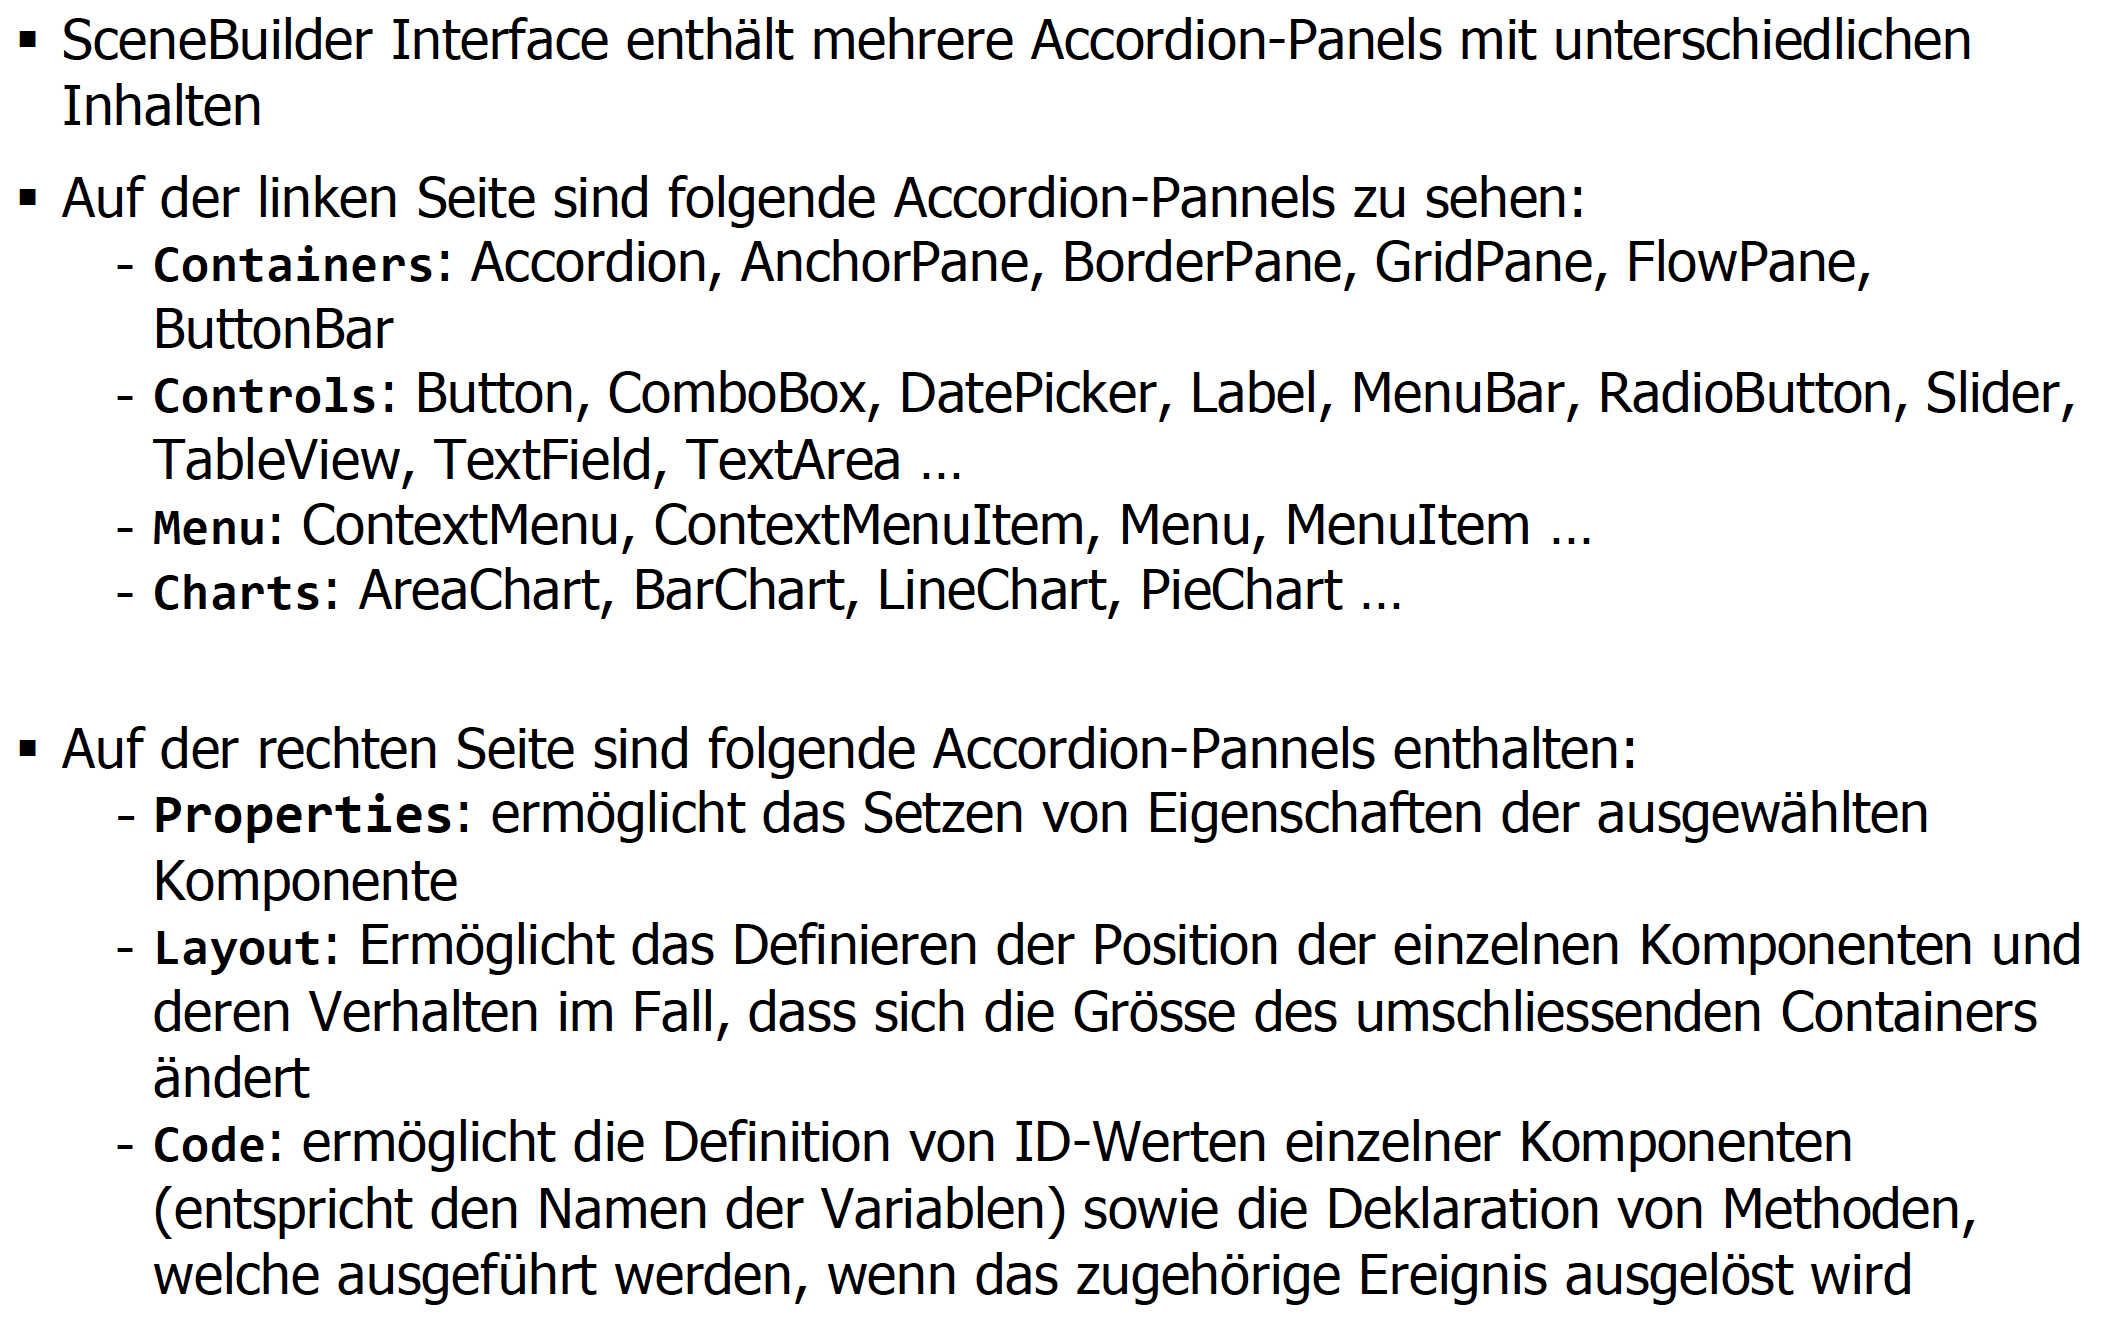
\includegraphics[keepaspectratio, width=\textwidth]{img/gui/scenebuilder_comp.png}
			\caption{Accordion-Panels-Beschreibungen des SceneBuilder}
			\label{fig:scene02}
		\end{figure}
		\noindent
		\begin{center}
			\textbf{Die Folien für die JavaFX-Demo aus der Vorlesung \\
			sind am Ende dieser Zusammenfassung ersichtlich!}
		\end{center}
		\noindent
		SceneBuilder für einfache, schnelle JavaFX-GUI-Erstellung verwendbar, braucht anfangs evtl. etwas Übung.
		In der Foliendemo wurde einfaches Beispiel gezeigt, welches nur ein Formular (View) benötigt.
		Das Vorgehen kann analog auf die Erstellung von GUIs mit mehreren Formularen (Views) übertragen werden.
		Es käme noch die Navigation hinzu, welche bspw. mithilfe einer \texttt{MenuBar}-Komponente realisiert werden kann.
		
	\newpage
	\section{Persistierung - JPA \& OR Mapping}
	
		\subsection{Sie wissen, was unter OR Mapping zu verstehen ist und welche Vor- und Nachteile OR Mapping mit sich bringt}
		
			\subsubsection{Varianten zur Persistierung von Objekten in relationale Datenbanken}
			
				\paragraph{Variante 1: Persistierung mit SQL und JDBC}
				
					\begin{itemize}
						\item \textbf{Vorgehen:} Programmierer schreibt SQL-Queries, um Abbildung von Objekten auf Tabellen sicherzustellen
						\item Programmieren mit Objekten, Verwaltung dieser aber mithilfe von Relationen (Tabellen) realisiert \\
						$\rightarrow$ Objekte nicht mehr als logische, zusammengehörende Einheiten, werden i.d.R. auf mehrere Tabellen verteilt, zusammengehörende Teile müssen verknüpft werden (Fremdschlüssel-Konzept)
						\item Abbildung von Objekten auf Relationen und Beziehungen (inkl. Vererbung)\\
						$\rightarrow$ von Hand mithilfe von SQL
						\item \textbf{Nachteil:} Aufwändig, viel SQL und fehleranfällig
					\end{itemize}
				
				\paragraph{Variante 2: OR-Mapping (object relational)}
				
					\begin{itemize}
						\item \textbf{Vorgehen:} Programmierer arbeitet mit Objekten\\
						$\rightarrow$ SQL-Teil (Abbildung Objekte auf Tabellen) von OR Mapper übernommen
						\item Job des Entwicklers:\\
						Erstellt, speichert und holt vollwertige(-ständige) Objekte aus Datenbank
						\item Entwickler arbeitet mit Objekten, hat mit SQL nichts mehr zu tun (ausser Ausnahmefälle)
						\item Abbildung von Objekten auf Relationen mit SQL übernimmt seperate Instanz (OR-Mapper)
					\end{itemize}
		
		\subsection{Sie kennen die wichtigsten von JPA zur Verfügung gestellte Annotationen und deren Bedeutung}
		
			\subsubsection{Java Persistence API (JPA)}
			
			\begin{quote}
				\textit{The Java Persistence API (JPA) is a Java specification for accessing, persisting, and managing data between Java objects / classes and a relational database.\\
				\\
				JPA is now considered the standard industry approach for Object to Relational Mapping (ORM) in the Java Industry.\\
				\\
				JPA itself is just a specification, not a product; it cannot perform persistence or anything else by itself. JPA is just a set of interfaces, and requires an implementation.}
			\end{quote}
		
			\begin{itemize}
				\item JPA-\textbf{Provider} stellen eine konkrete Implementation der JPA-Spezifikation zur Verfügung, solche Provider wären:\\
				EclipseLink, Hibernate, OpenJPA, DataNucleus etc.
				\item JPA-Vorteile:
					\begin{itemize}
						\item ermöglicht Speichern von Daten auf objektorientierte Weise (als Objekte)
						\item einfach im Gebrauch, nicht von einem Provider abhängig
						\item stellt Portabilität von Anwendungen sicher
						\item kann mit JEE \& JSE verwendet werden
					\end{itemize}
				\item Anforderungen an JPA-Provider:
					\begin{itemize}
						\item Verwaltung von Verbindungen zu DB
						\item Mapping von Klassen und deren Felder auf Tabellen \& Spalten (Attribute)
						\item Abbildung von Beziehungen
						\item Verwaltung von Relationen (Tabellen)
						\item Objektorientierte Suchmöglichkeiten zur Verfügung stellen
					\end{itemize}
			\end{itemize}
		
			\newpage
			
			\subsubsection{JPA mit EclipseLink}
			
			\begin{itemize}
				\item EclipseLink: JPA-Referenzimplementierung\\
				\textit{(Zusammen mit Hibernate der meistverwendete JPA-Provider, lustige Zusatzinfo höhö)}
				\item JPA-Annotationen: Sprachelemente, ermöglichen Einbindung von Metadaten in Quellcode\\
				(Beginnen mit @, gefolgt von Annotationsnamen, können auch Parameter (Attribute) enthalten)
				\item Beispiele:
					\begin{itemize}
						\item \texttt{@Entity}
						\item \texttt{@Id}
						\item \texttt{@GeneratedValue(strategy=GenerationType.AUTO)}
						\item \texttt{@Column(name="GEB\_DATUM")}
						\item \texttt{@JoinTable(name="student\_lerngruppe")}
						\item \texttt{@ManyToMany(mappedBy="projects")}
					\end{itemize}
			\end{itemize}
		
			\begin{figure}[!htb]
				\centering
				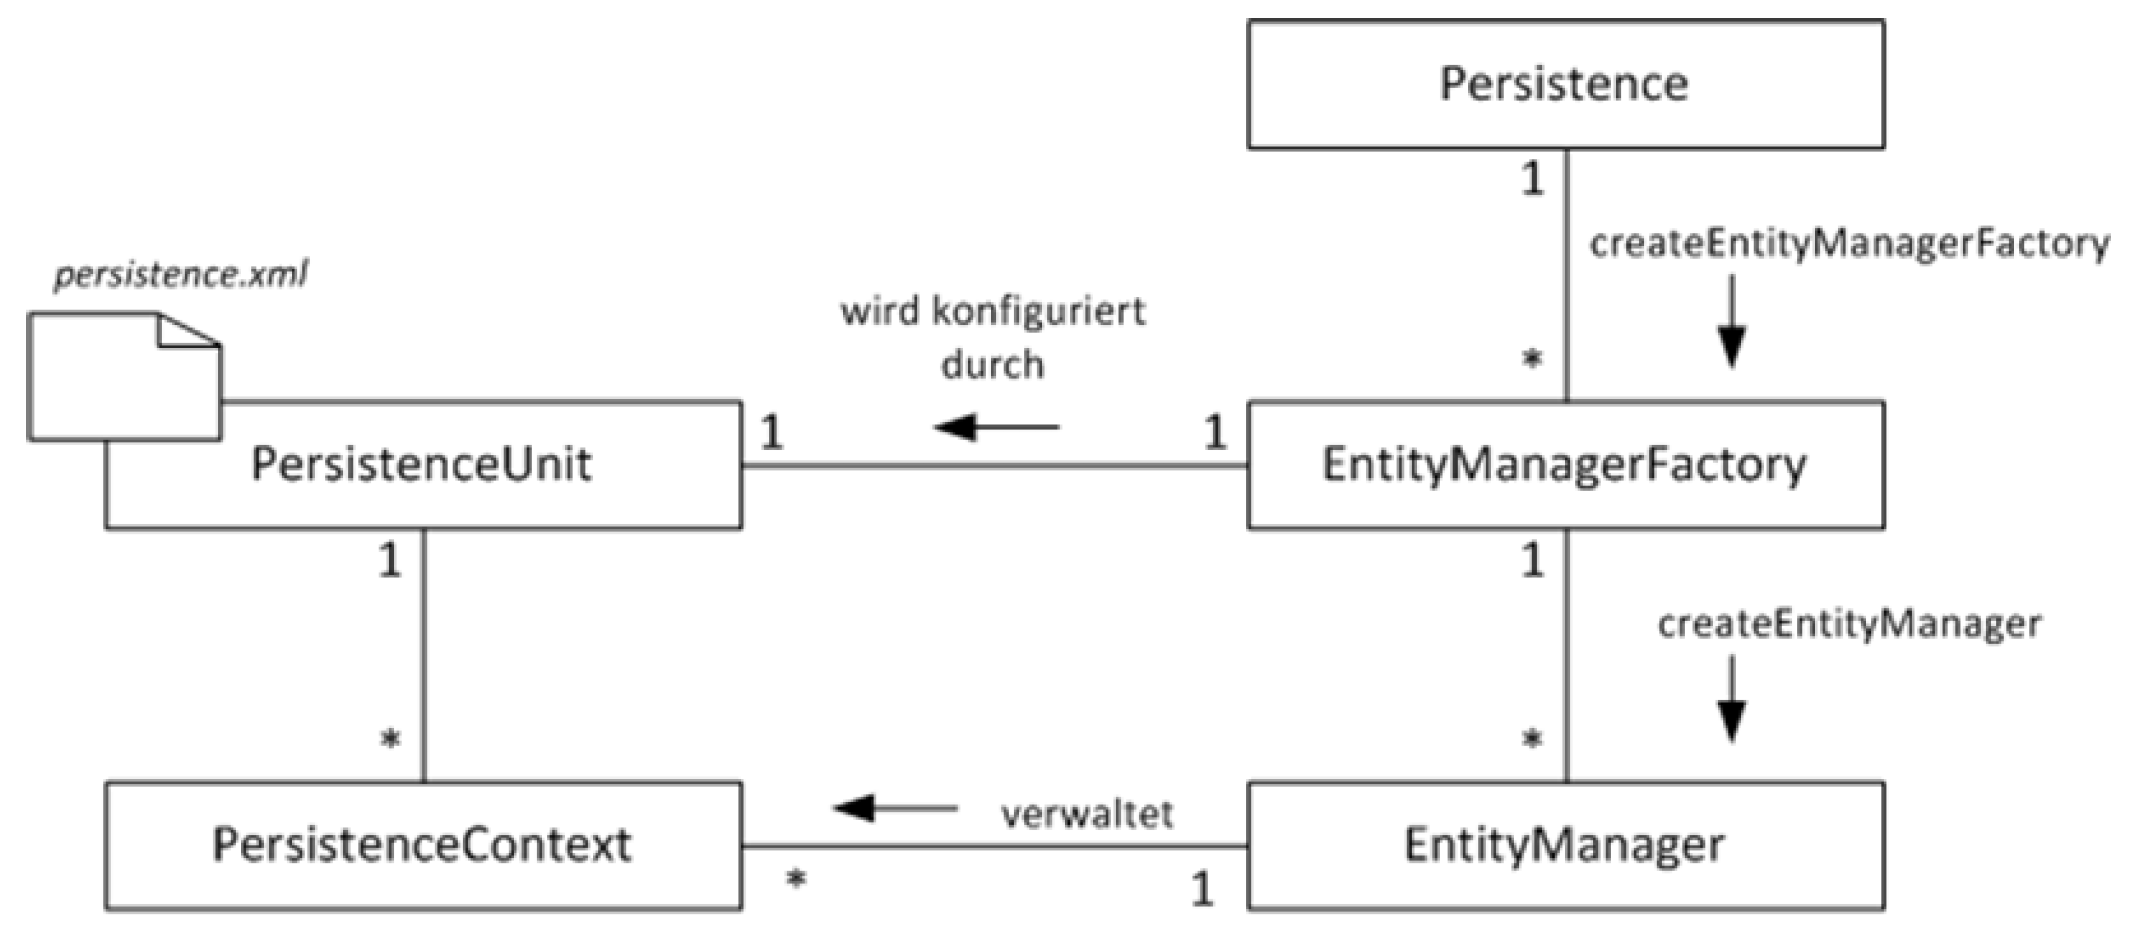
\includegraphics[keepaspectratio, height=4cm]{img/persistence/grundbegriffe.png}
				\caption{Grundbegriffe und Klassen von JPA}
				\label{fig:jpa_base}
			\end{figure}
		
			\begin{itemize}
				\item \textbf{Entity}:\\
						Bezeichnung für Objekte (POJO), deren Zustände in DB verwaltet werden soll\\
						\textit{Beispiel:} \texttt{Adresse, Person, Buch}...
						
				\item \textbf{Klasse} \texttt{javax.persistence.Persistence}:\\
						Benötigt Namen der "PersistenceUnit"\\
						Für Erzeugung des DB Schema und \texttt{EntityManagerFactory}-Instanz zuständig
						
				\item \textbf{Klasse} \texttt{javax.persistence.EntityManagerFactory}:\\
						Für Erzeugung von \texttt{EntityManager}-Instanzen zuständig
						
				\item \textbf{Klasse} \texttt{javax.persistence.EntityManager}:\\
						Von \texttt{EntityManagerFactory} erstellt\\
						\textit{(Erstellung kann in seperate Util-Klasse ausgelagert werden)}\\
						Für Verwaltung von Entities (PersistenceContext) zuständig
						
				\item \textbf{Klasse} \texttt{javax.persistence.EntityTransaction}:\\
						Für Verwaltung von Transaktionen zuständig \textit{(no shit)}
						
				\item \textbf{Persistenzkontext} (PersistenceContext):
						\begin{itemize}
							\item Summer aller vom EntityManager verwalteten Entities
							\item Kann sich (nach Bedarf) ändern: Entities hinzufügen/entfernen etc.
							\item Zuständiger EntityManager muss immer wissen, in welchem Zustand sich eine Entity die er verwaltet (in seinem Kontext) befindet\\
							(Ist sie neu hinzugefügt aber noch nicht gespeichert, geändert etc. worden)
						\end{itemize}
			\end{itemize}
		
			\paragraph{Konfiguration}
			
			JPA-Provider benötigt Infos für Verbindung zur DB, Datenbewirtschaftung etc.
			Können entweder in statischer Datei \texttt{persistence.xml} oder dynamisch während Laufzeit konfiguriert werden. 
			\texttt{persistence.xml} muss im Verzeichnis \texttt{META-INF} abgelegt sein.
			Dynamische Variante (wird weniger genutzt) kann bspw. zum Wechsel von Datenbanken während Laufzeit genutzt werden.
			
			\newpage
		
			\begin{figure}[!htb]
				\centering
				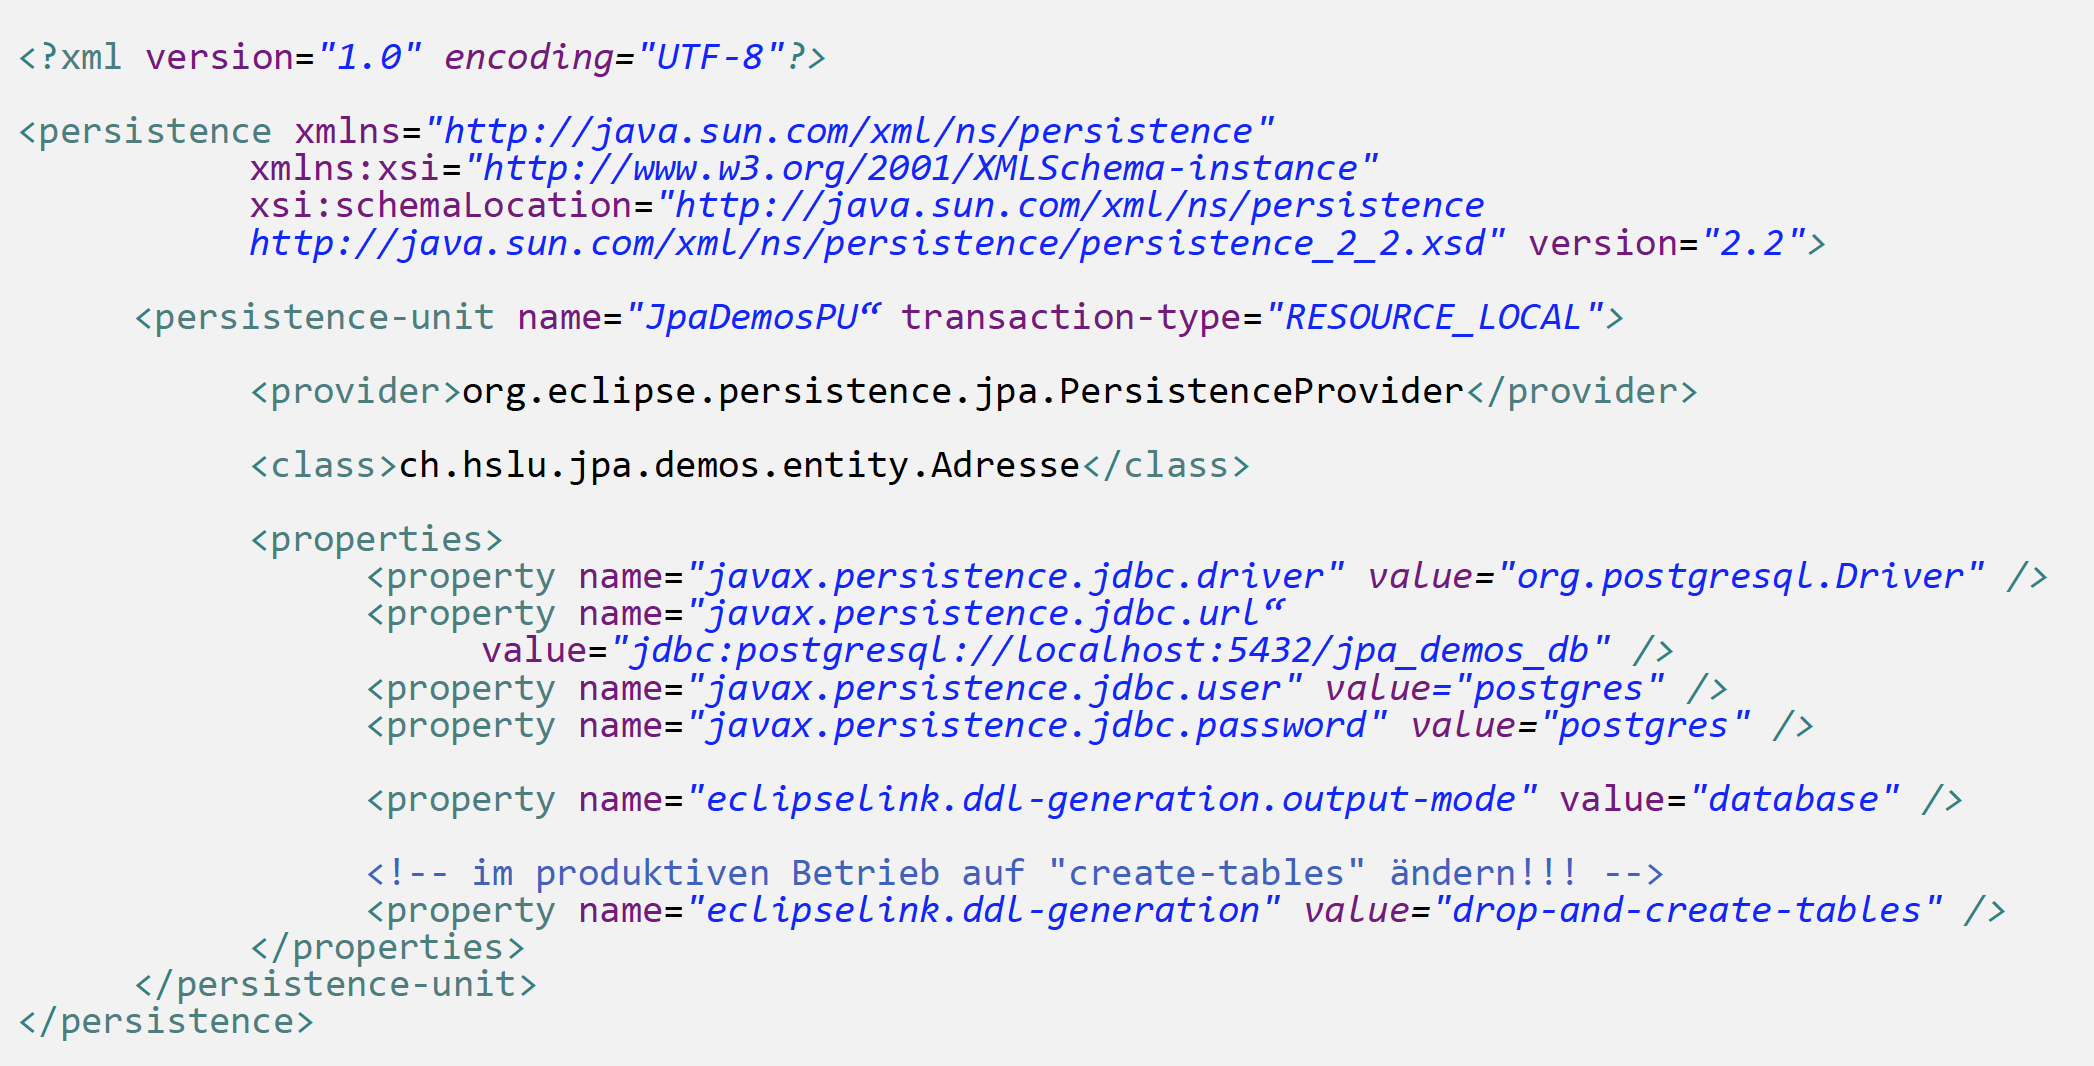
\includegraphics[keepaspectratio, height=6.5cm]{img/persistence/persistencexml.png}
				\caption{Beispiel einer Konfigurationsdatei \texttt{persistence.xml}}
				\label{fig:persistence_xml}
			\end{figure}
			
			\paragraph{EntityManager}
			
			\begin{figure}[!htb]
				\centering
				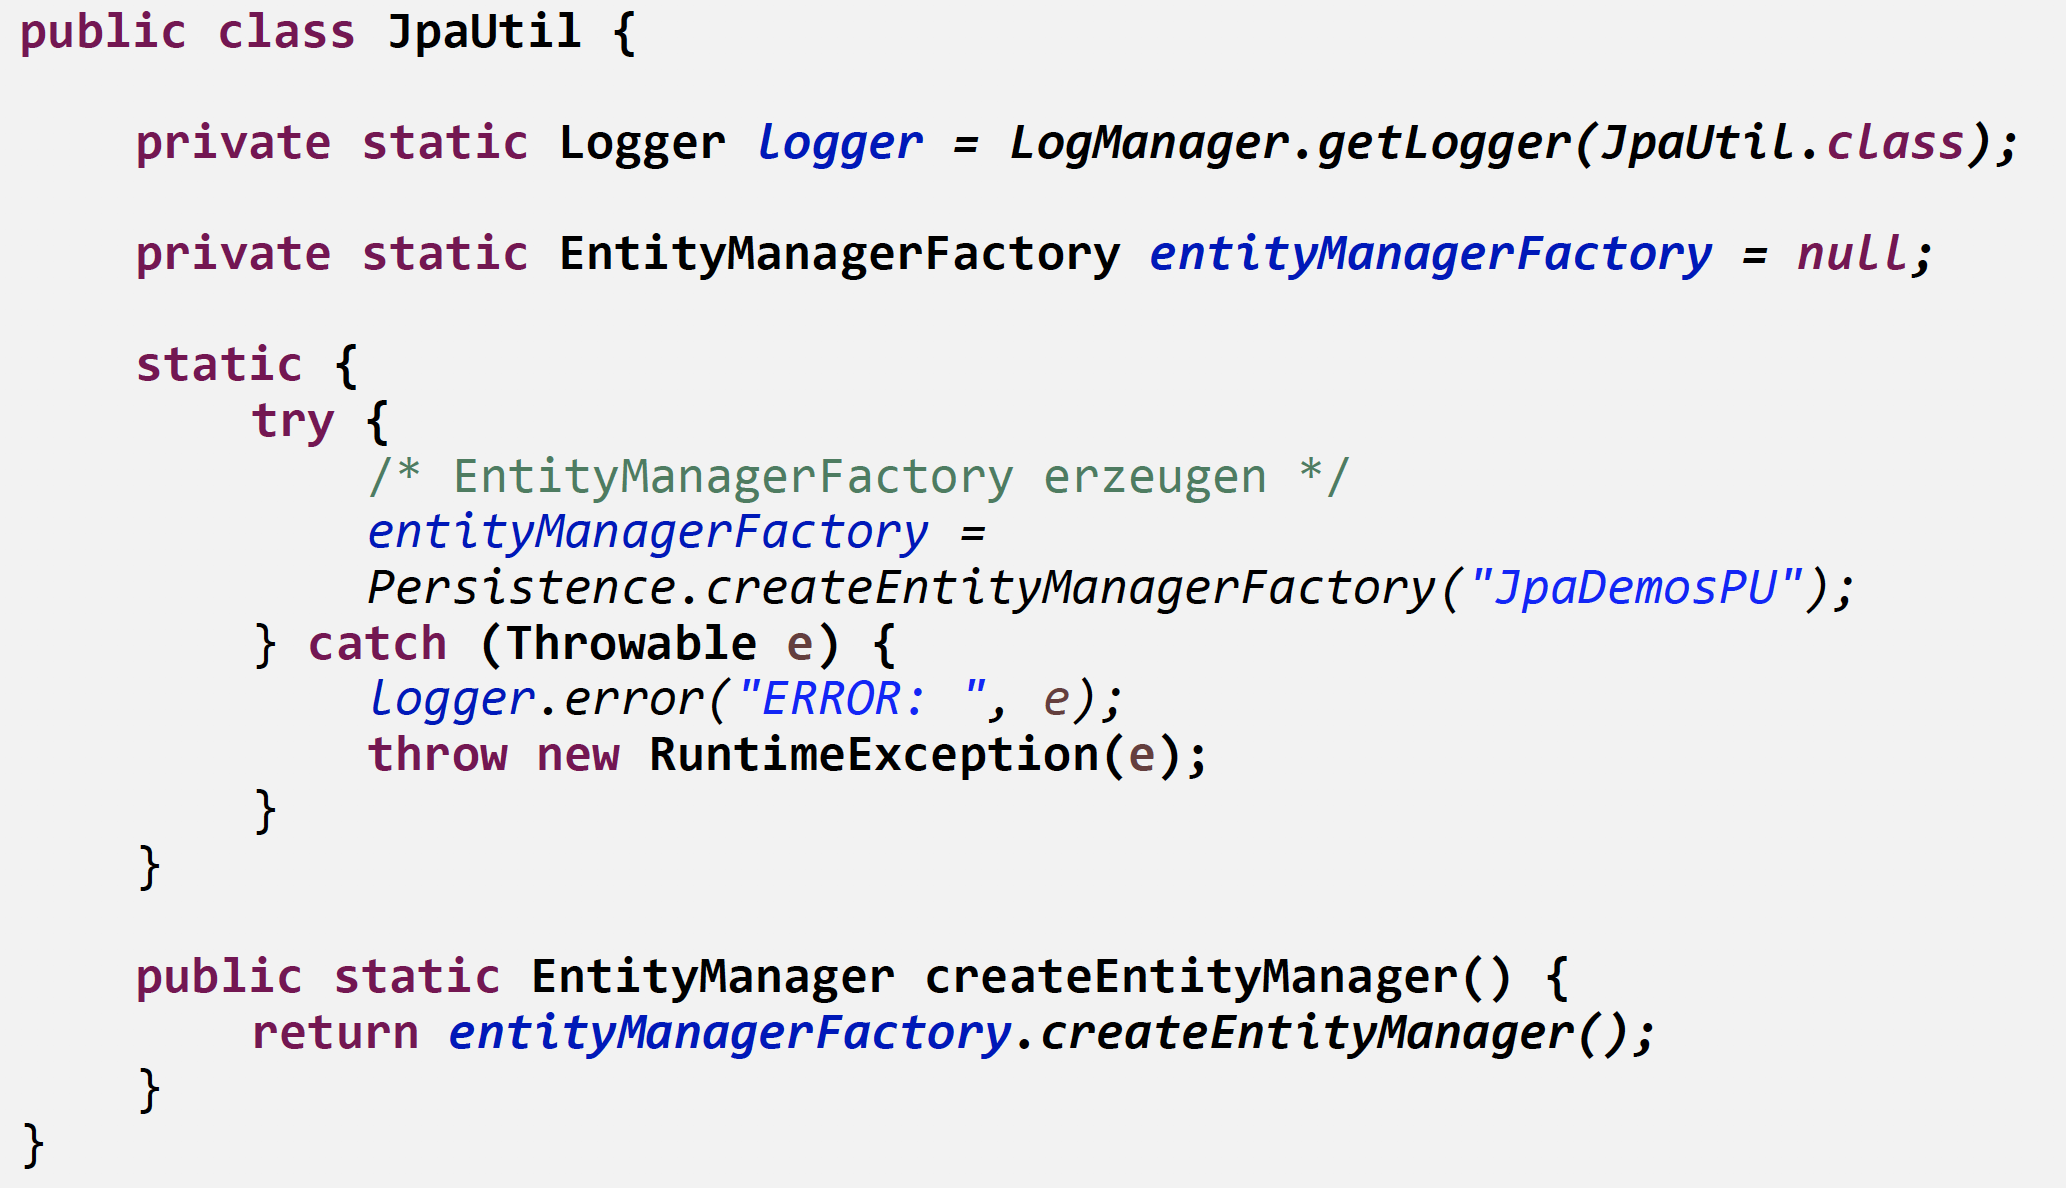
\includegraphics[keepaspectratio, height=5cm]{img/persistence/entityutil.png}
				\caption{Beispiel einer Util-Klasse, die \texttt{EntityManager}-Instanzen erzeugt}
				\label{fig:entity_util}
			\end{figure}
		
			\begin{itemize}
				\item Entity Manager CRUD-Methoden:
					\begin{itemize}
						\item \texttt{void persist (Object entity)}
						\item \texttt{<T> T find(Class<T>, Object primaryKey)}
						\item \texttt{<T> T merge (T entity)}
						\item \texttt{void remove(Object entity)}
						\item ja gäbe scheinbar noch andere\\
					\end{itemize}
			\end{itemize}
		\noindent
		Beispiel zum Speichern einer Adresse-Entity:
		
		\begin{lstlisting}
Adresse adr = new Adresse("Seestr. 2", 6000, "Luzern");
EntityManager em = JpaUtil.createEntityManager(); // Beispiel Util-Klasse siehe oben

em.getTransaction().begin();		// Transaktion starten
em.persist(adr);						// Entity speichern (persistieren)
em.getTransaction().commit();	// Transaktion abschliessen (commit)
em.close();
		\end{lstlisting}
		
		\newpage
		
		\paragraph{Entity}
		
		\begin{figure}[!htb]
			\centering
			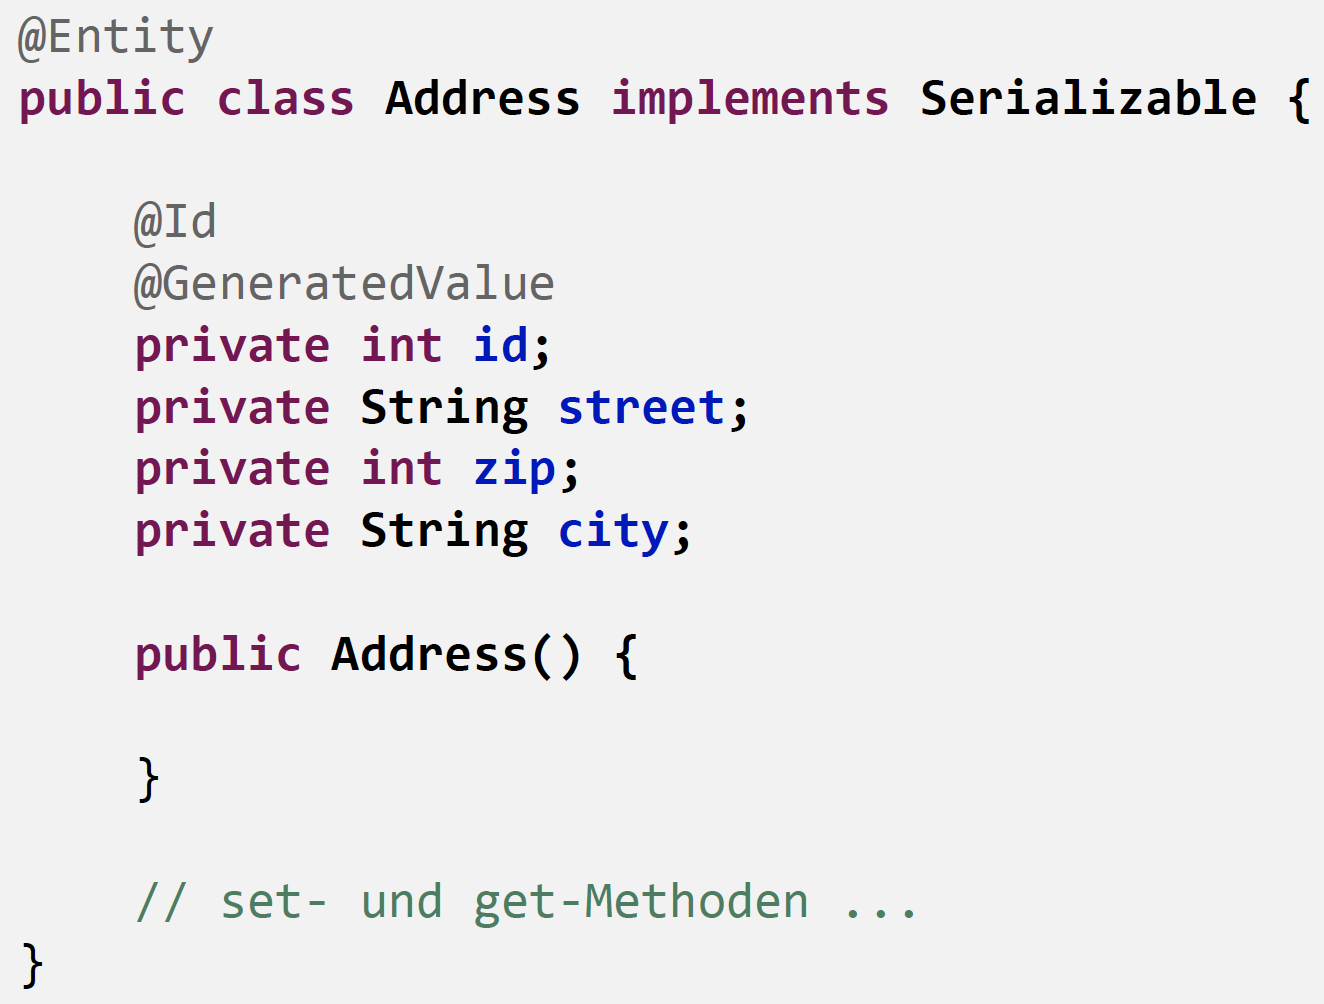
\includegraphics[keepaspectratio, height=4cm]{img/persistence/entity.png}
			\caption{Beispiel Entity-Klasse mit entsprechenden Annotationen}
			\label{fig:entity}
		\end{figure}
	
		Klasse, deren Instanzen als Entitäten in DB geschrieben werden sollen, muss mit entsprechenden Annotationen versehen werden.
		
		\subsection{Sie wissen, wie die Beziehungen zwischen Objekten (ausgehend von einem Klassendiagramm oder von dem gegebenen Code) nach JPA Regeln korrekt spezifiziert werden}
		
			\subsubsection{Assoziationen}
			
			JPA-Annotationen für Definition von Beziehungen:
			\begin{itemize}
				\item \texttt{@OneToOne} \qquad\quad[ 1 : 1 ]
				\item \texttt{@OneToMany} \qquad [ 1 : m ]
				\item \texttt{@ManyToOne} \qquad [ m : 1 ]
				\item \texttt{@ManyToMany} \qquad[ m : m ]
				\item Für minimale Kardinalität ist auch Null erlaubt, mithilfe von Annotation:\\
				\texttt{@Column (nullable=true)}\\
				\texttt{private String telefon;}
			\end{itemize}
		
			\begin{figure}[!htb]
				\centering
				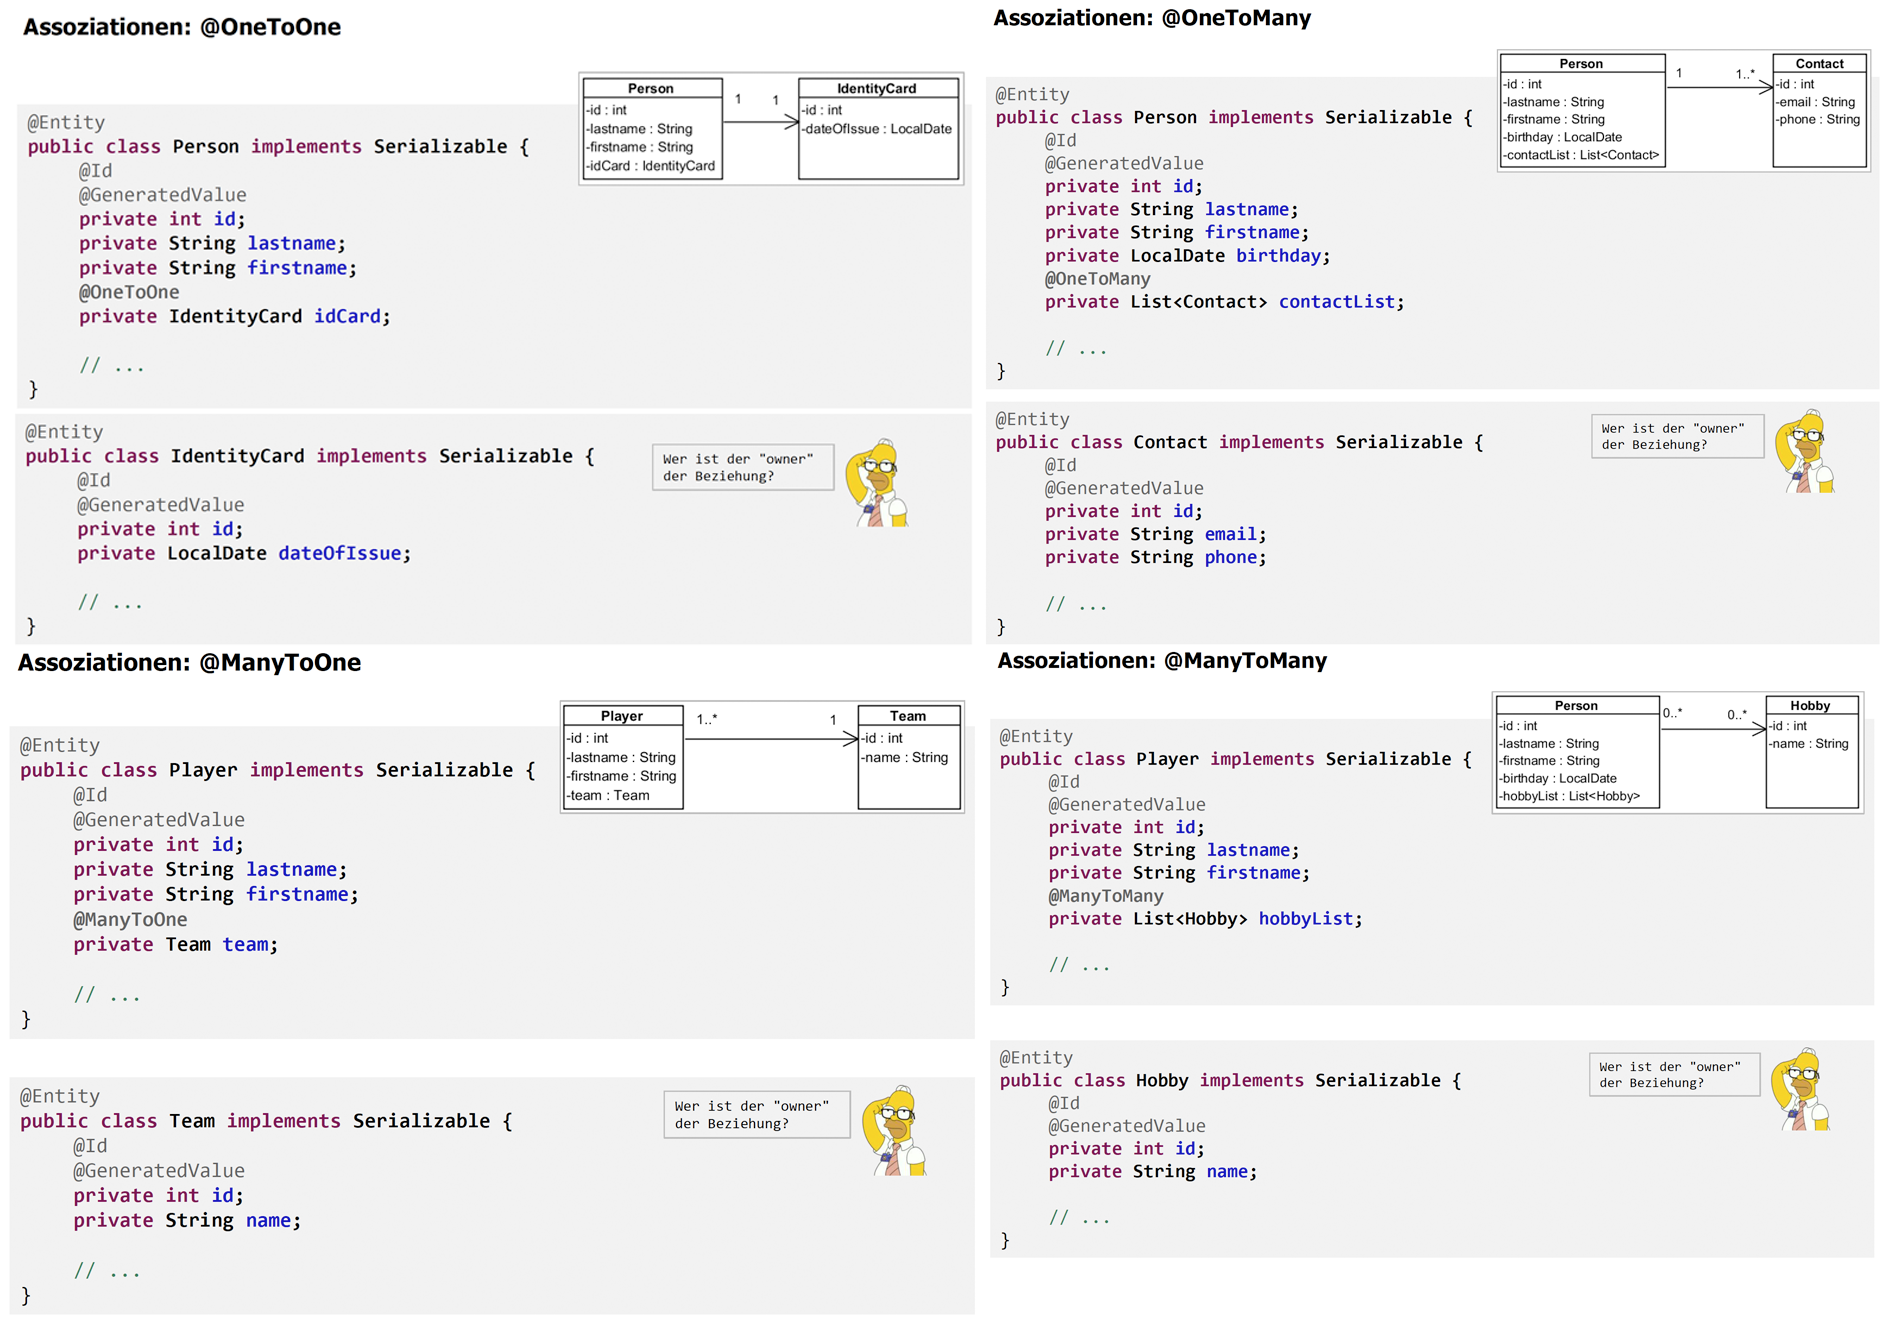
\includegraphics[keepaspectratio, width=.9\textwidth]{img/persistence/associations.png}
				\caption{Codebeispiele für die verschiedenen Beziehungen}
				\label{fig:associations}
			\end{figure}
			
			\newpage
			
			\subsubsection{Vererbung}
			
			\begin{figure}[!htb]
				\centering
				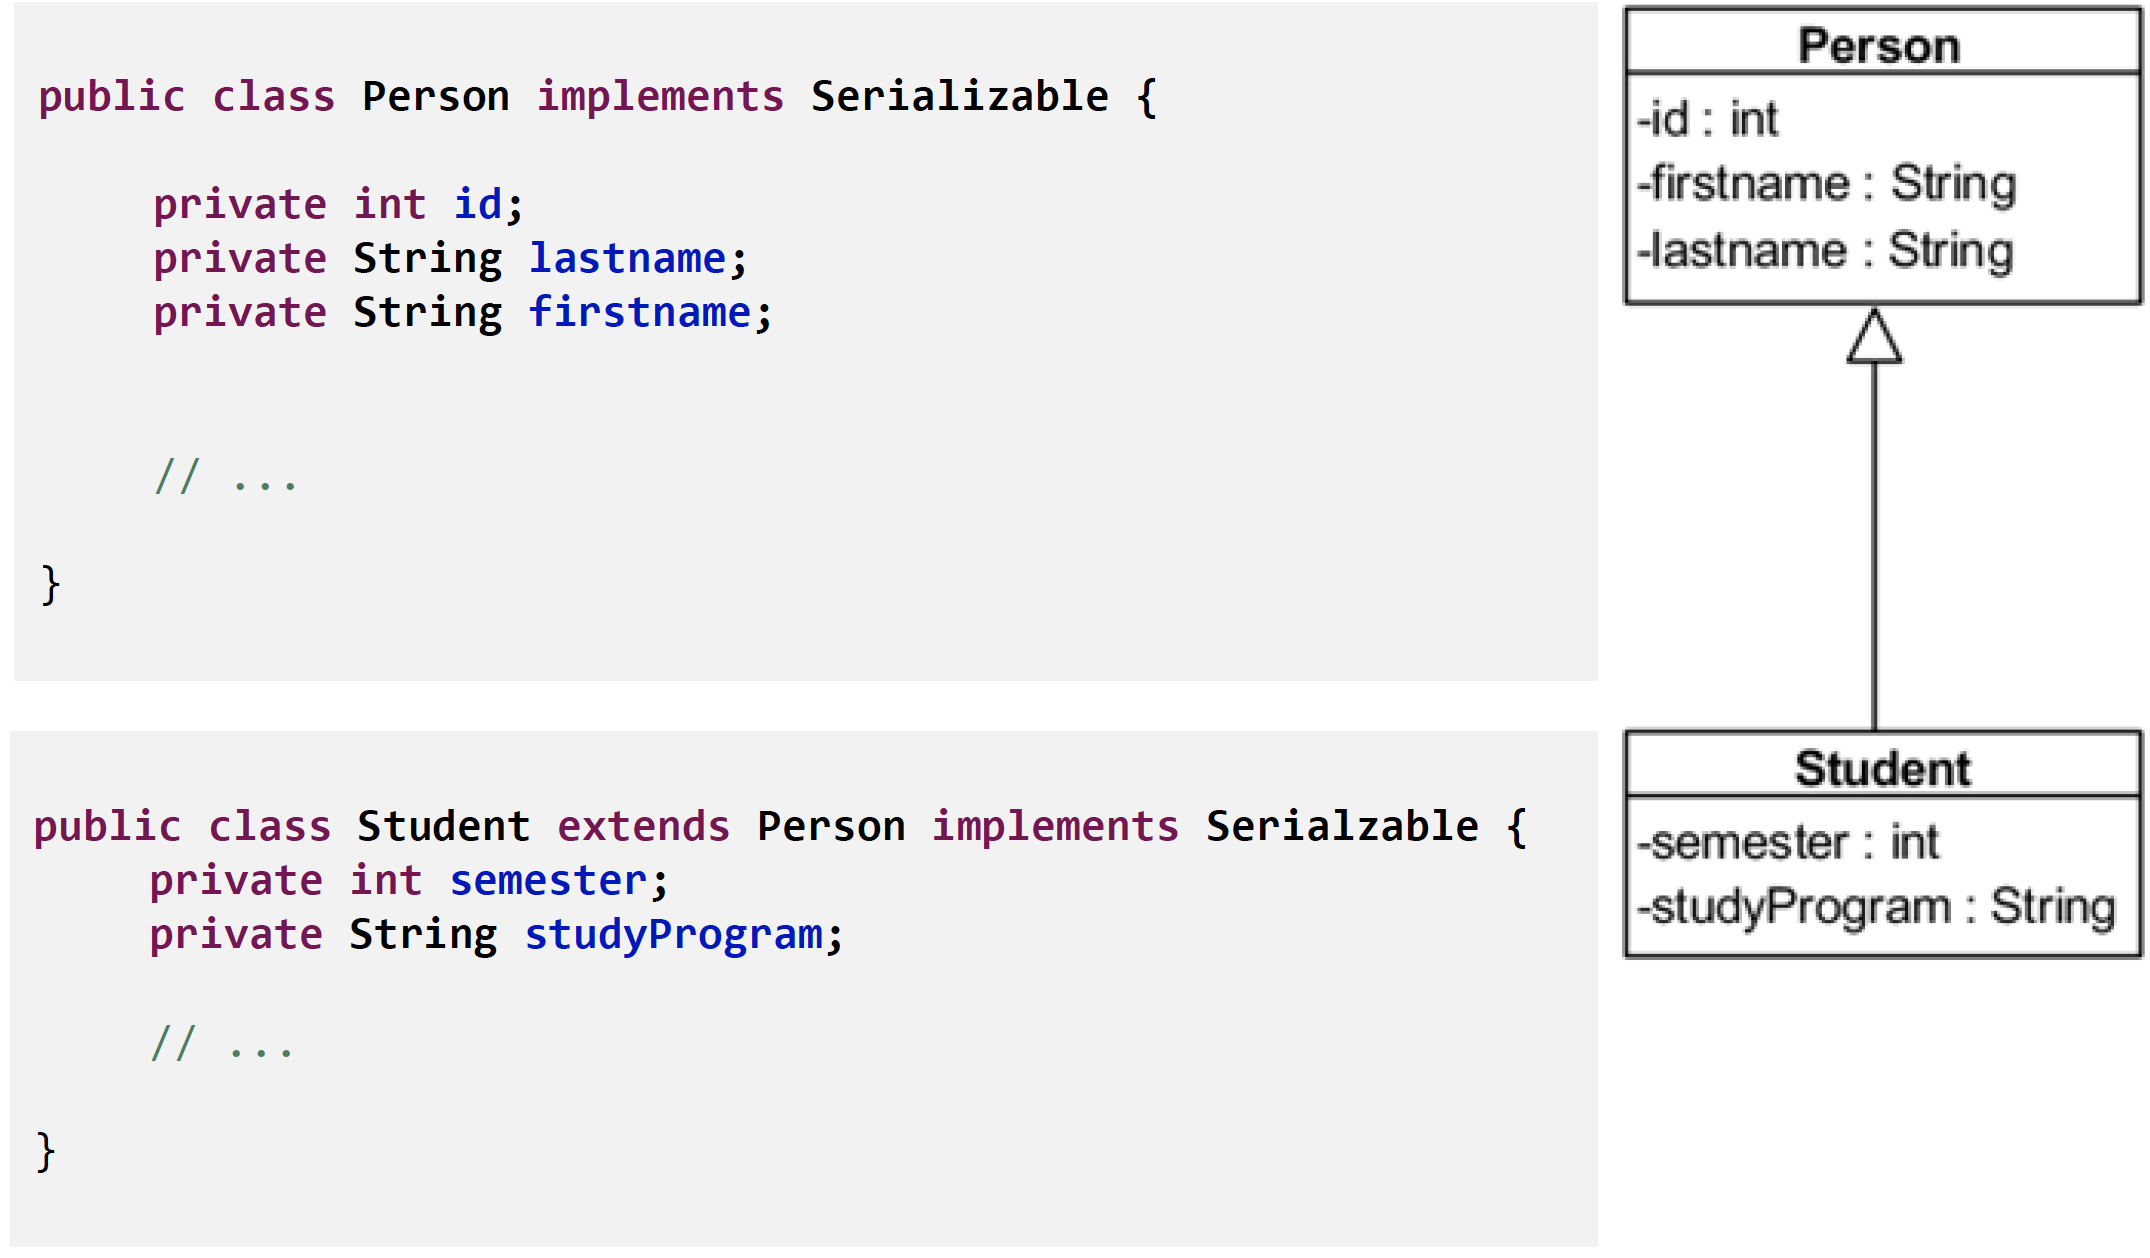
\includegraphics[keepaspectratio, height=6cm]{img/persistence/inheritance.png}
				\caption{Simples Beispiel von Vererbung zw. Entitäten}
				\label{fig:inheritance}
			\end{figure}
		
			\paragraph{InheritanceType SINGLE\_TABLE}
			
			Alle Klassen der Vererbungshierarchie werden in einer Tabelle abgebildet.
			Mit einer "Diskriminator"-Spalte (hier \texttt{typ}) wird der Datentyp markiert.\\
			JPA-Annotation: \texttt{@Inheritance(strategy=InheritanceType.SINGLE\_TABLE)}
			
			\begin{figure}[!htb]
				\centering
				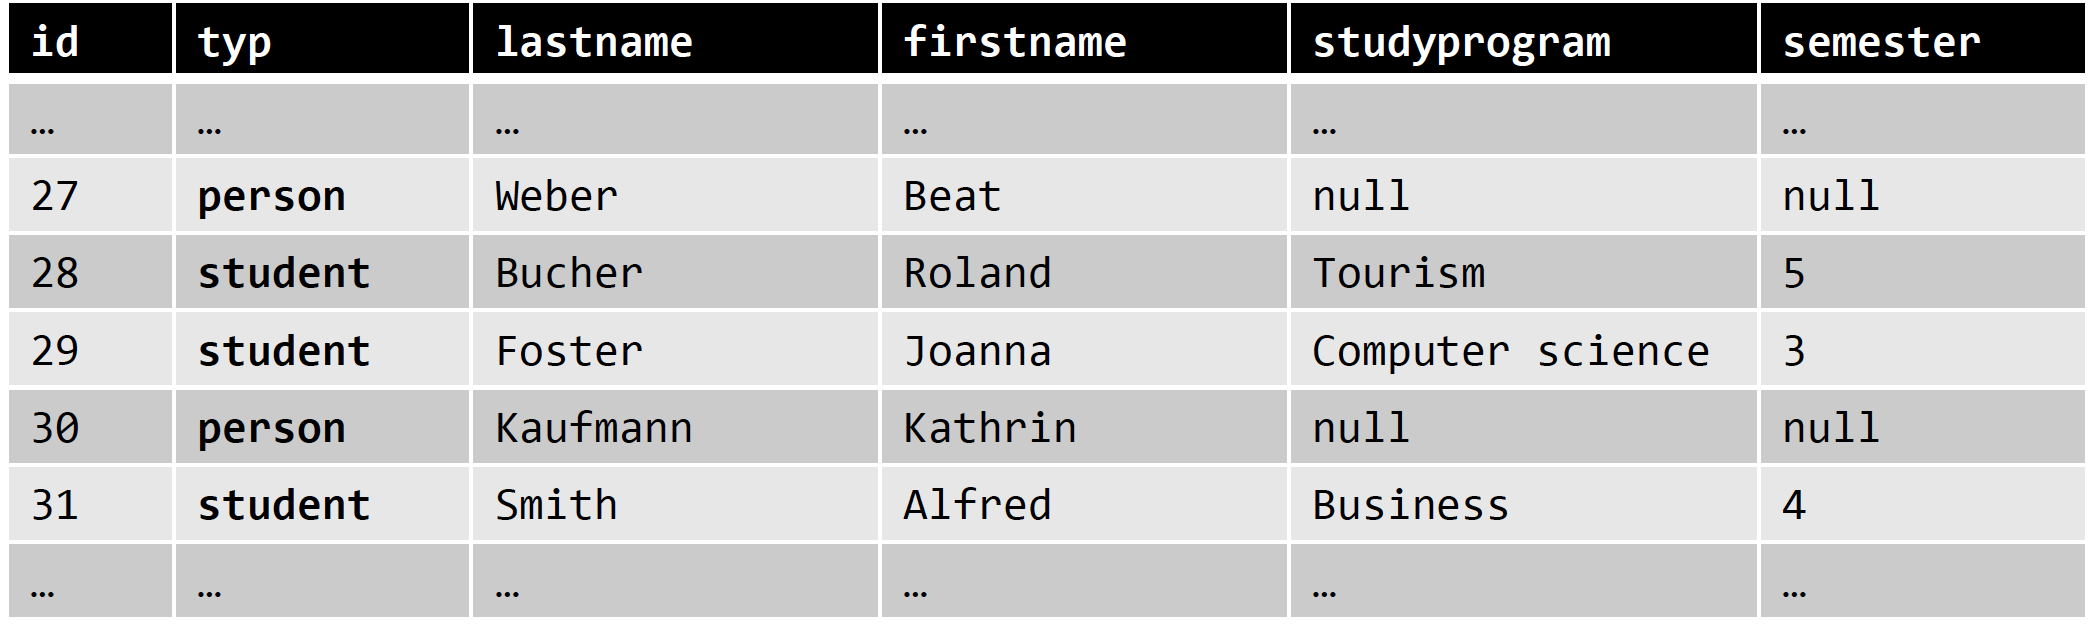
\includegraphics[keepaspectratio, height=4cm]{img/persistence/single_table.png}
				\caption{SINGLE\_Table Vererbung in einer Tabelle}
				\label{fig:single_table}
			\end{figure}
		
			\paragraph{InheritanceType JOINED}
			
			Pro konkrete und abstrakte Klasse einer Vererbungshierarchie wird eine Tabelle angelegt.
			Das Objekt wird dann über \textbf{Sup}- und \textbf{Sub}-Tabellen "verteilt".\\
			JPA-Annotation der Oberklasse: \texttt{@Inheritance(strategy=InheritanceType.JOINED)}
			
			\begin{figure}[!htb]
				\centering
				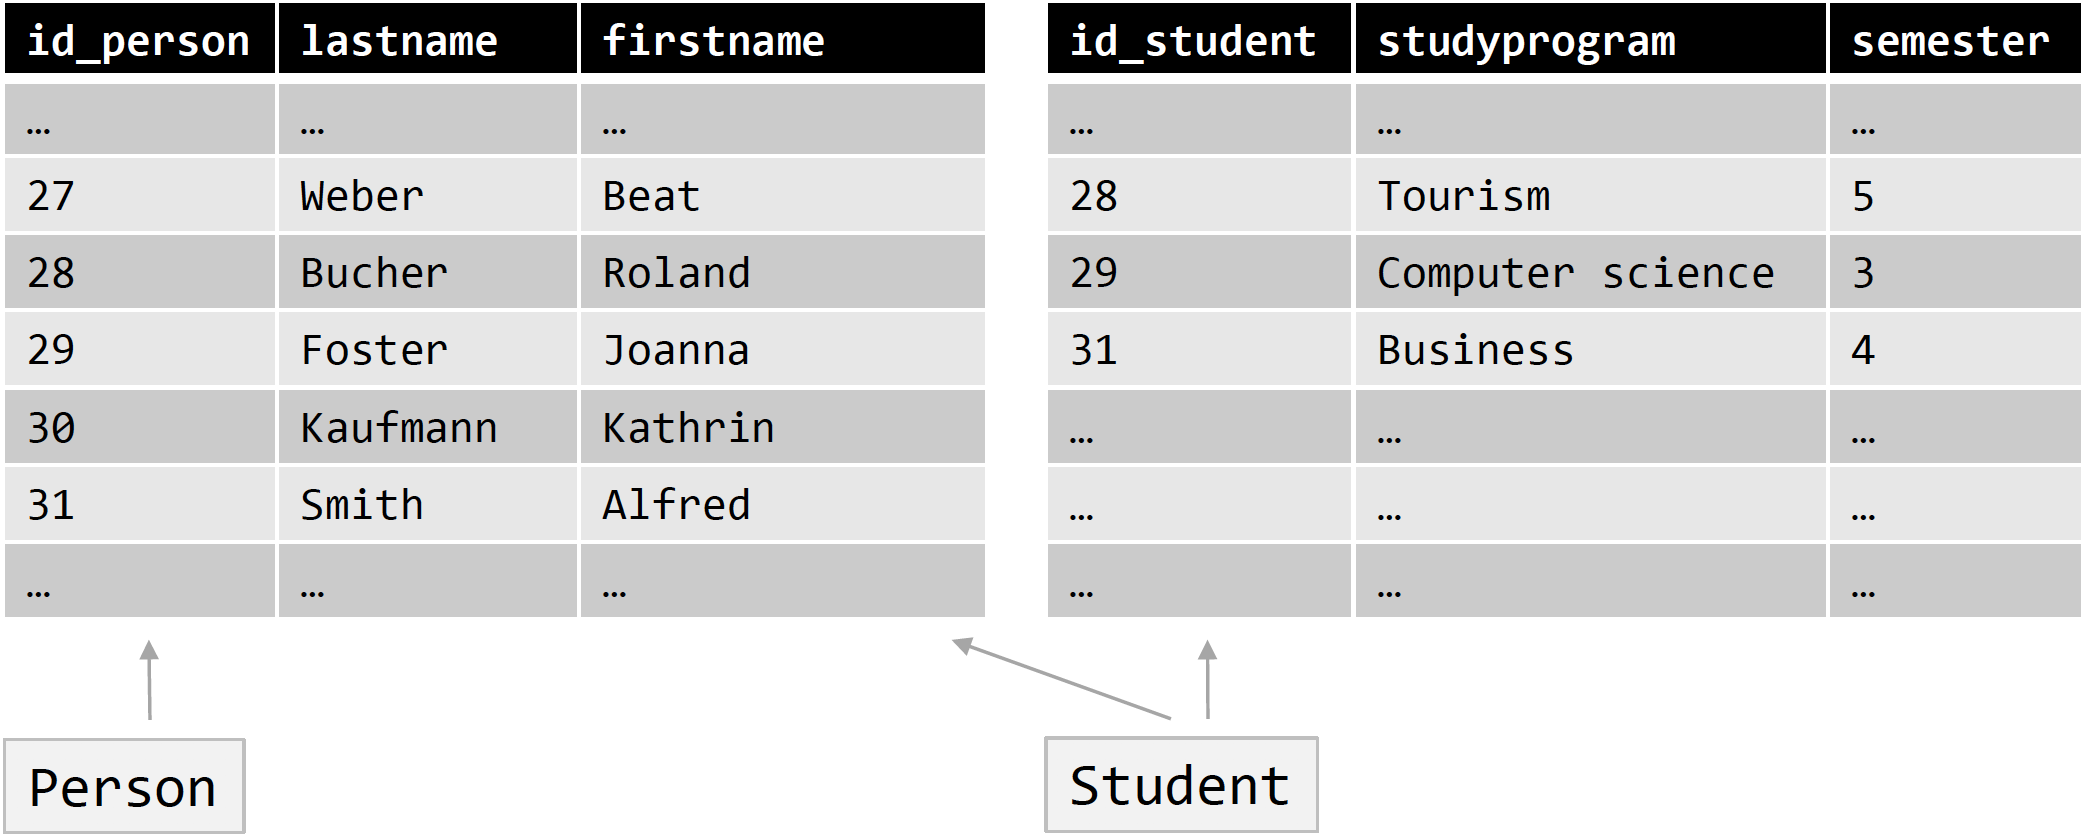
\includegraphics[keepaspectratio, height=4cm]{img/persistence/joined.png}
				\caption{JOINED Vererbung "verteilt" auf zwei Tabellen}
				\label{fig:joined}
			\end{figure}
		
			\newpage
		
			\begin{figure}[!htb]
				\centering
				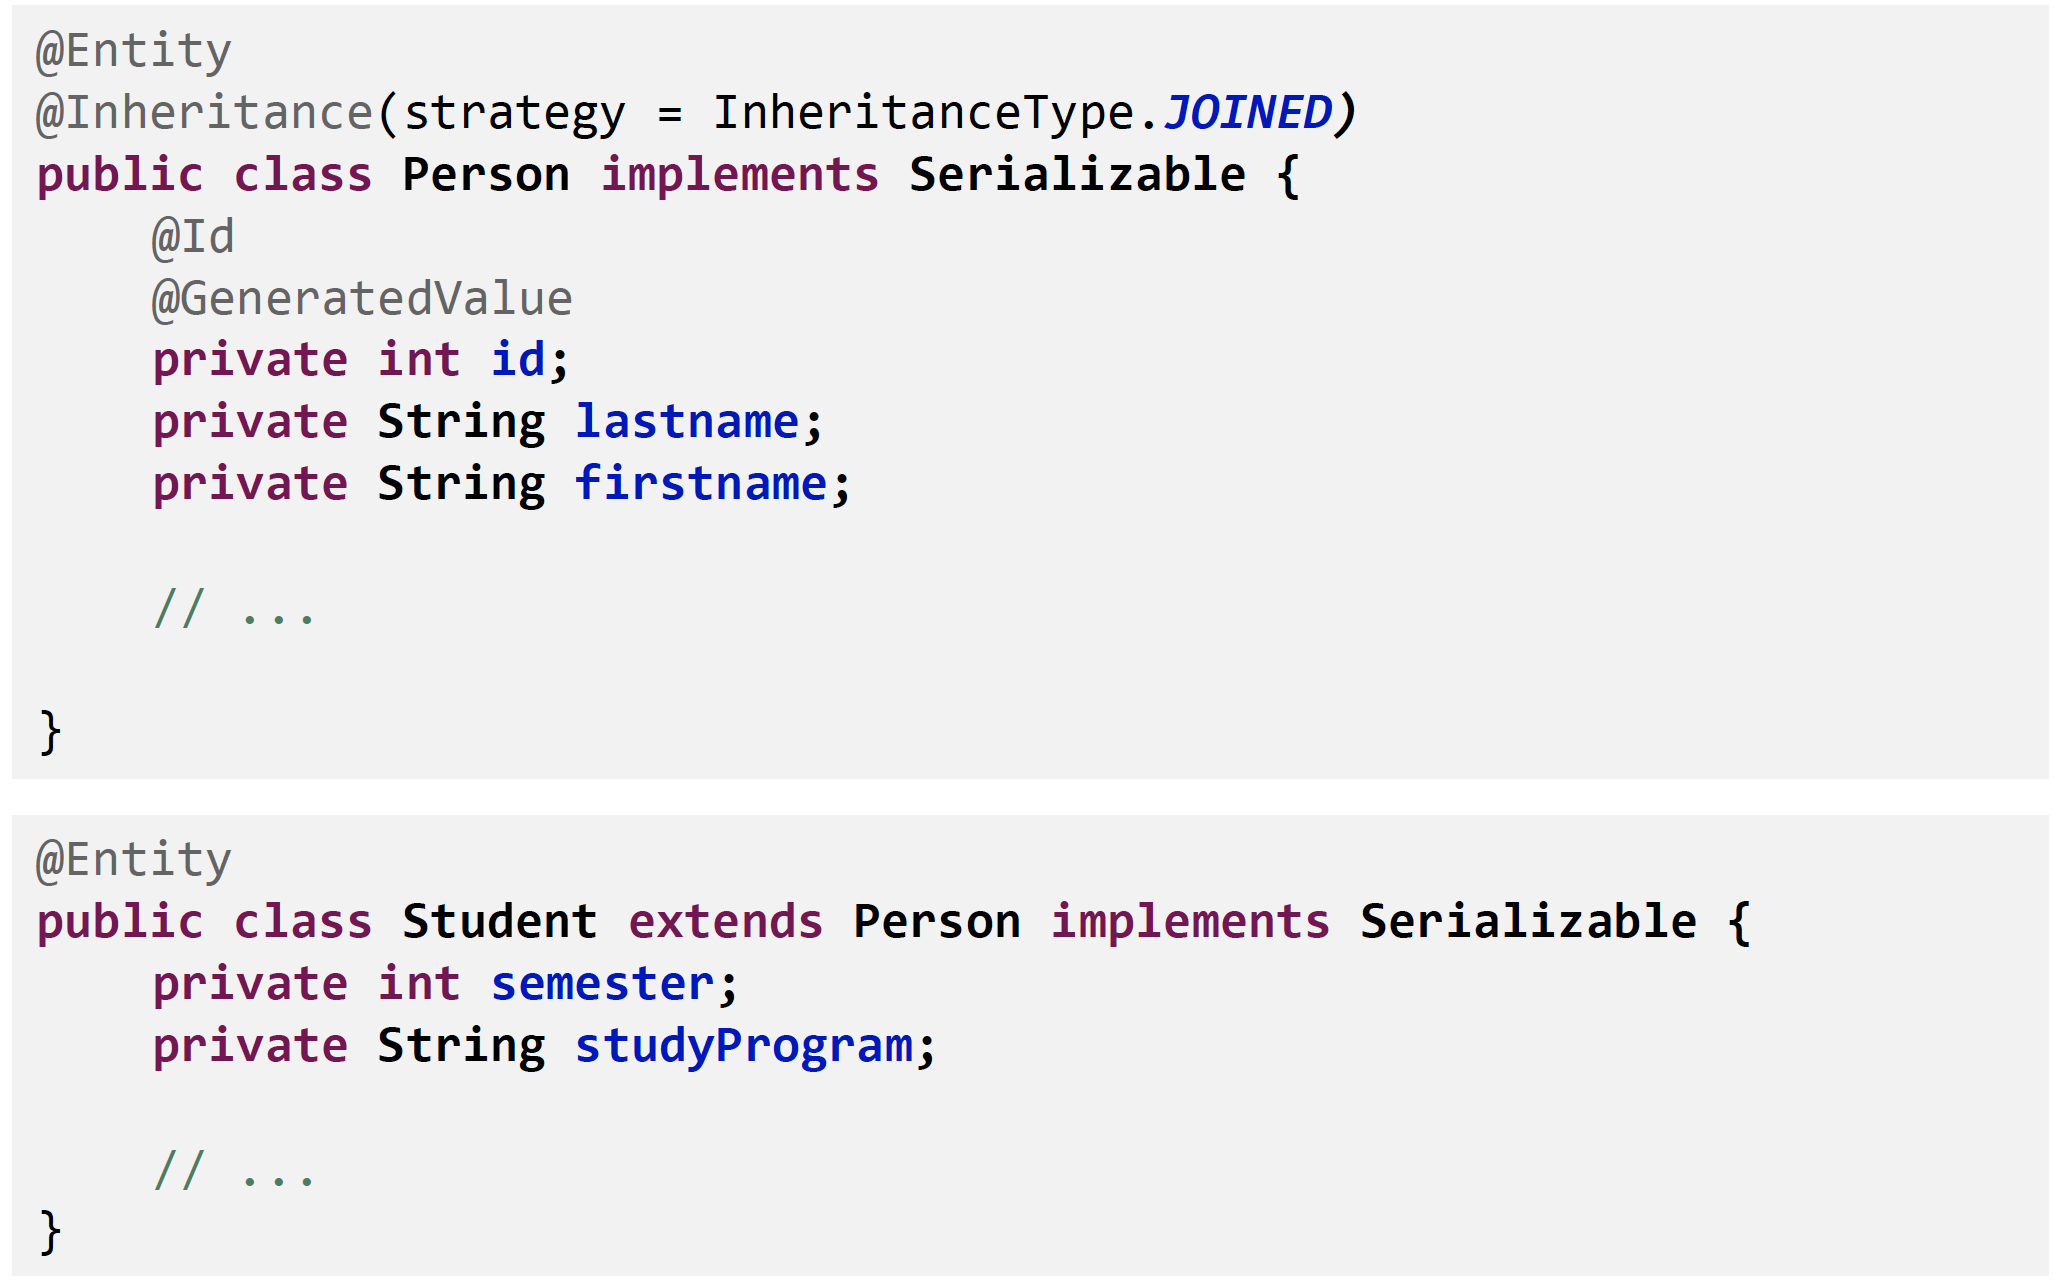
\includegraphics[keepaspectratio, height=6cm]{img/persistence/joined_code.png}
				\caption{Konkretes Code-Beispiel für eine JOINED-Vererbung}
				\label{fig:joined_code}
			\end{figure}
		
		
		\subsection{Sie sind in der Lage, OR Mapping in einem konkreten Fall korrekt anzuwenden}
		
		Jo locker, das setti scho chönne.
		Soscht luegi mis SWDE-Projekt aa, \textbf{det hanis schliesslech gmacht}.
		Soscht heds ide Folie no di folgend Üebig:\\
		\textit{Vervollständigen Sie die im Rahmenprogramm zur Verfügung gestellten Klassen so, das deren Instanzen in eine Datenbank mit Hilfe eines OR Mappers persistiert werden können. 
		Die für die Beziehungen relevanten Informationen können dem Klassendiagramm entnommen werden.}
		
		\begin{figure}[!htb]
			\centering
			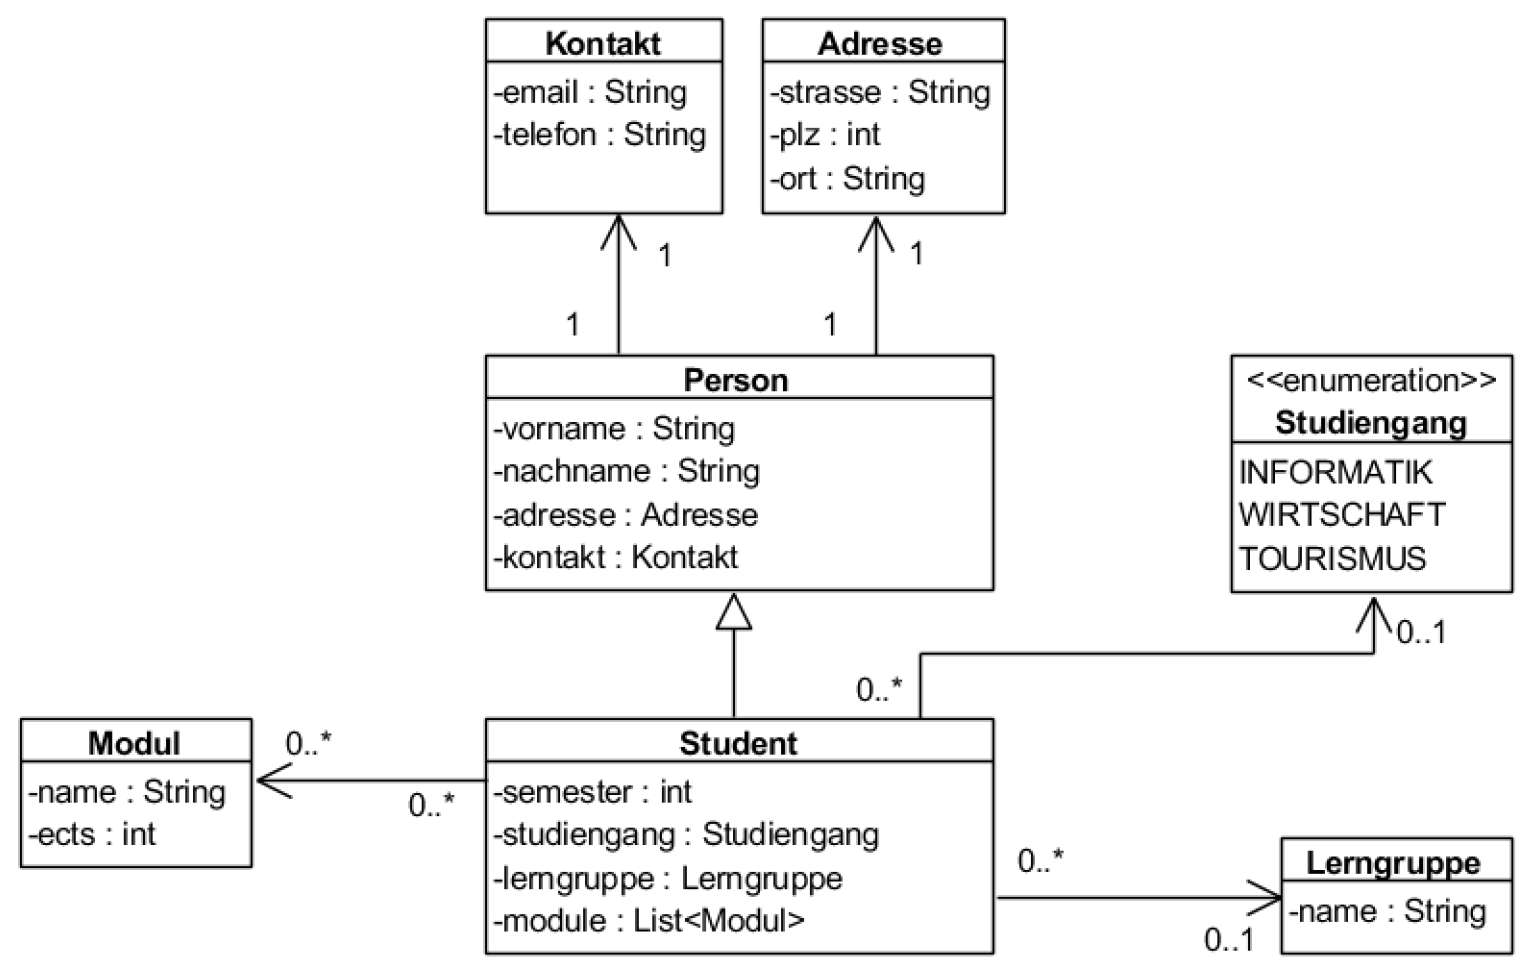
\includegraphics[keepaspectratio, height=9cm]{img/persistence/jpa_exercise.png}
			\caption{Rahmendiagramm zur Vorlesungsübung}
			\label{fig:jpa_exercise}
		\end{figure}
		
				
	\newpage
	\section{Persistierung - Java Persistence Query Language (JPQL)}
		
		\subsection{Sie wissen, wie mit Hilfe von JPQL Daten aus einer relationalen Datenbank abgefragt werden können (data retrieving)}
		
		\begin{itemize}
			\item JPQL erinnert an SQL, ist jedoch komplett objektorientiert
			\item Nicht Case-Sensitive (abgesehen von Klassen- und Attributnamen)
			\item JPQL-Abfrage: mindestens ein SELECT- und ein FROM-Block
				\begin{itemize}
					\item \texttt{SELECT}: Daten angeben, welche aus Wertebereich des FROM-Block zurückgeliefert werden
					\item \texttt{FROM}: Wertebereich \& Identifikationsvariablen definieren,\\
						können in anderen Blöcken wiederverwendet werden
				\end{itemize}
			\item \textbf{Beispiel:}\\
			\texttt{SELECT p FROM Person p}\\
			\textit{Person}: Name der Klasse\\
			\textit{p}: Identifikationsvariable\\
		\end{itemize}
		\noindent
		Einschränkung der Datenmenge mit WHERE, wobei unterschiedliche Operatoren verwendet werden können. Eine einfache Abfrage mit WHERE wäre:
		
		\begin{lstlisting}
SELECT p
FROM Person p
WHERE p.vorname='Hansli'
		\end{lstlisting}
		\noindent
		Abfragen mit logischen \& relationalen Operatoren:
		\begin{lstlisting}
SELECT p FROM Person p WHERE p.name='Meier' AND p.vorname LIKE '%and'
SELECT a FROM Adresse a WHERE a.plz > 10000 OR ort LIKE '%ns'
		\end{lstlisting}
		\noindent
		Anfrage mit Menge-Operatoren:
		\begin{lstlisting}
SELECT a FROM Adresse a WHERE a.plz between '6000' AND '7000'
SELECT a FROM Adresse a WHERE a.plz IN ('6000', '6010', '6030', '6048')
		\end{lstlisting}
		\noindent
		JPQL erlaubt auch Verwendung von String-Methoden:
		\begin{lstlisting}
SELECT p
FROM Person p
WHERE p.vorname.length() > 5

SELECT substring(p.vorname, 2, 5)
FROM Person p
WHERE p.vorname.toLowerCase()='hanspeter'
		\end{lstlisting}
		\noindent
		Sortieren der Ergebnismenge kann mit ORDER BY vorgenommen werden:
		\begin{lstlisting}
SELECT p FROM Person p WHERE p.name='Meier' ORDER BY p.vorname DESC
SELECT a FROM Adresse a ORDER BY a.plz ASC
SELECT p FROM Person p ORDER BY p.adresse ASC
		\end{lstlisting}
		
		\newpage
		
		\subsection{Sie kennen die wesentlichen JPQL Konstrukte (Query, TypedQuery , NamedQuery) und deren Eigenschaften}
		
				\paragraph{Query}
				
					\begin{itemize}
						\item Interface \texttt{javafx.persistence.Query}:\\ 
						Zentrale Schnittstelle bei JPA-Abfragen\\
						Wird immer benötigt, wenn Entity-Primärschlüssel nicht zur Verfügung steht
						\item Query-Instanz mithilfe EntityManager erstellen:\\
								\texttt{Query query = em.createQuery("SELECT p FROM Person p");}
						\item Abfrage kann mit einer der folgenden Methoden durchgeführt werden:
						\begin{itemize}
							\item \texttt{Object getSingleResult()}
							\item \texttt{List getResultList()}
						\end{itemize}
						\item Rückgabewert beider Methoden ist nicht typisiert, muss gecastet werden (Typumwandlung):\\
						\texttt{Person p = (Person) query.getSingleResult();}
					\end{itemize}
				
				\paragraph{TypedQuery}
				
					\begin{itemize}
						\item Interface \texttt{javafx.persistence.TypedQuery<T>}:\\
						Ermöglicht Abfragen mit typisiertem Rückgabewert
							\begin{itemize}
								\item \texttt{T getSingleResult()}
								\item \texttt{List<T> getResultList()}
							\end{itemize}
						\item TypedQuery wird vom EntityManager erstellt:\\
							\texttt{TypedQuery<Person> tQuery = em.createQuery("SELECT p FROM Person p", Person.class);}
						\item Rückgabewert typisiert, muss nicht mehr gecastet werden:\\
						\texttt{Person p = tQuery.getSingleResult();}\\
					\end{itemize}
					Konkretes Beispiel:
					\begin{lstlisting}
List<Person> personListe = tQuery.getResultList();

for (Person p : personliste) {
	System.out.println(p.getName() + " " + p.getVorname());
}
					\end{lstlisting}
					JPA ermöglicht Erstellung von "parametrisierten" Abfragen.
					Dabei werden die aktuellen Parameterwerte (Argumente) nachträglich in die Abfrage "injiziert". Beispiel:
					\begin{lstlisting}
TypedQuery<Person> tQuery = em.createQuery("SELECT p FROM Person p
																WHERE p.name=:name
																AND p.vorname=:vorname",
																Person.class);
tQuery.setParameter("name", "Pechvogel");
tQuery.setParameter("vorname", "Hansli");
					\end{lstlisting}
					Alternative Möglichkeit:
					\begin{lstlisting}
TypedQuery<Person> tQuery = em.createQuery("SELECT p FROM Person p
																WHERE p.name=?1 AND p.vorname=?2",
																Person.class);
tQuery.setParameter(1, "Pechvogel");
tQuery.setParameter(2, "Hansli");
					\end{lstlisting}
				
				\newpage
				
				\paragraph{NamedQueries}
					
					\begin{itemize}
						\item JPA kann benannte Abfragen definieren (named queries)
						\item Werden mit eindeutigen Namen versehen \& können beliebig wiederverwendet werden
						\item Abfragen mit vordefinierten Abfragestrings
						\item Üblich in der zugehörigen Entity-Klasse definiert
						\item Trennung der Abfragen vom Code $\rightarrow$ positive Auswirkung auf Codeorganisation\\
					\end{itemize}
					Definitionsbeispiel:
					\begin{lstlisting}
@Entity
@NamedQuery(name = "Student.findBySemester",
					query = "SELECT e FROM Student e WHERE e.semester=:semester")
@NamedQuery(name = "Student.findByLastnameAndFirstname",
					query = "SELECT e FROM Student e WHERE e.lastname=:lastname
									AND e.firstname=:firstname")
public class Student implements Serializable(
		// Implementierung
)
					\end{lstlisting}
					Diese \texttt{NamedQueries} können beliebig oft vom \texttt{EntityManager} verwendet werden, Beispiel:
					\begin{lstlisting}
TypedQuery<Student> q = 
				em.createNamedQuery("Student.findBySemester", Student.class);
q.setParameter("semester", 5);
List<Student> studentList = q.getResultList();
					\end{lstlisting}
					Anzeige der Ergebnismenge:
					\begin{lstlisting}
for (Student s : studentList) {
		System.out.println(s.getLastName() + " " + 
		s.getFirstName() + ", Semester: + s.getSemester());
}
					\end{lstlisting}
					
				\paragraph{Fetching von Daten}
				
					\begin{itemize}
						\item JPA spezifiziert zwei Fetching-Strategien:
							\begin{itemize}
								\item \textbf{Lazy Load}: Daten erst aus DB laden, wenn sie benötigt werden
								\item \textbf{Eager Load}: Daten sofort vollständig laden
							\end{itemize}
						\item Angabe der Fetching-Strategien bei der Beziehung:\\
						\texttt{@OneToMany(fetch = FetchType.EAGER)\\
									private List<Student> studentList;}				
					\end{itemize}
			
				\paragraph{Kaskadierung von Aktionen}
				
					\begin{itemize}
						\item JPA stellt Möglichkeit zur Verfügung:\\
						Auf dem Aggregat-Objekt auszuführende Aktionen automatisch auf Teil-Objekt ausführen
						\item Beispiel A (Klasse \texttt{Verleger}):\\
						\texttt{@OneToMany (cascade = CascadeType.ALL)\\
						private List<Buch> buchListe;}
							\begin{itemize}
								\item Hier wird jede Aktion, die auf dem \texttt{Verleger} ausgeführt wird, auch auf allen \texttt{Buch}-Entities aus der \texttt{buchListe} ausgeführt
							\end{itemize}
						\item Beispiel B (Klasse \texttt{Person}):\\
						\texttt{@OneToOne (cascade = {CascadeType.PERSIST, CascadeType.REMOVE})\\
						private Adresse adresse;}
							\begin{itemize}
								\item Hier wird beim Speichern und Löschen einer \texttt{Person}-Entity auch die zugehörige \texttt{Adresse}-Entity gespeichert bzw. gelöscht
							\end{itemize}
					\end{itemize}
		
	\newpage
	\section{Kommunikation - Remote Method Invocation (RMI)}
	
		%TODO
		
		\subsection{Sie wissen, was unter RMI zu verstehen ist und kennen die Schwächen und Stärken von RMI}
		
		
		
		\subsection{Sie wissen, wie die Kommunikation zwischen Komponenten mit Hilfe von RMI realisiert wird}



		\subsection{Sie sind in der Lage, die Kommunikation zwischen einzelnen Komponenten einer verteilten Applikation mit Hilfe von RMI zu realisieren}
		
		
		
	
	\newpage
	\section{Web Services - REST}
	
		%TODO
		
		\subsection{Sie wissen, was unter Web Service zu verstehen ist und welche Vor- und Nachteile diese mit sich bringen}
		
		
		
		\subsection{Sie können die Eigenschaften von SAOP und REST basierenden Web Services}
		
		
		
		\subsection{Sie wissen, was unter REST zu verstehen ist und was mit RESTful gemeint ist}
		
		
		
		\subsection{Sie sind in der Lage, einen einfachen Web Service mit JAX RS zu implementieren}
		
		
		
		\subsection{Sie wissen, wie ein REST Client Programm als Java Programm erstellt wird und wie ein REST Web Service in einem konkreten Fall korrekt benutzt bzw. angesprochen werden kann}
		
		
		
		\subsection{Sie kennen die Unterschiede zwischen RMI und Web Services im Kontext der Kommunikation in einer verteilten Anwendung}
		
		
		
		\subsection{Sie sind in der Lage zu entscheiden, welche Middleware sich in einem konkreten Fall besser eignen würde}
		
		
		
		
	\newpage	
	\section{Zusammenfassung auf Folien}
	
		%TODO A LOT
		
		
		
	\newpage
		
	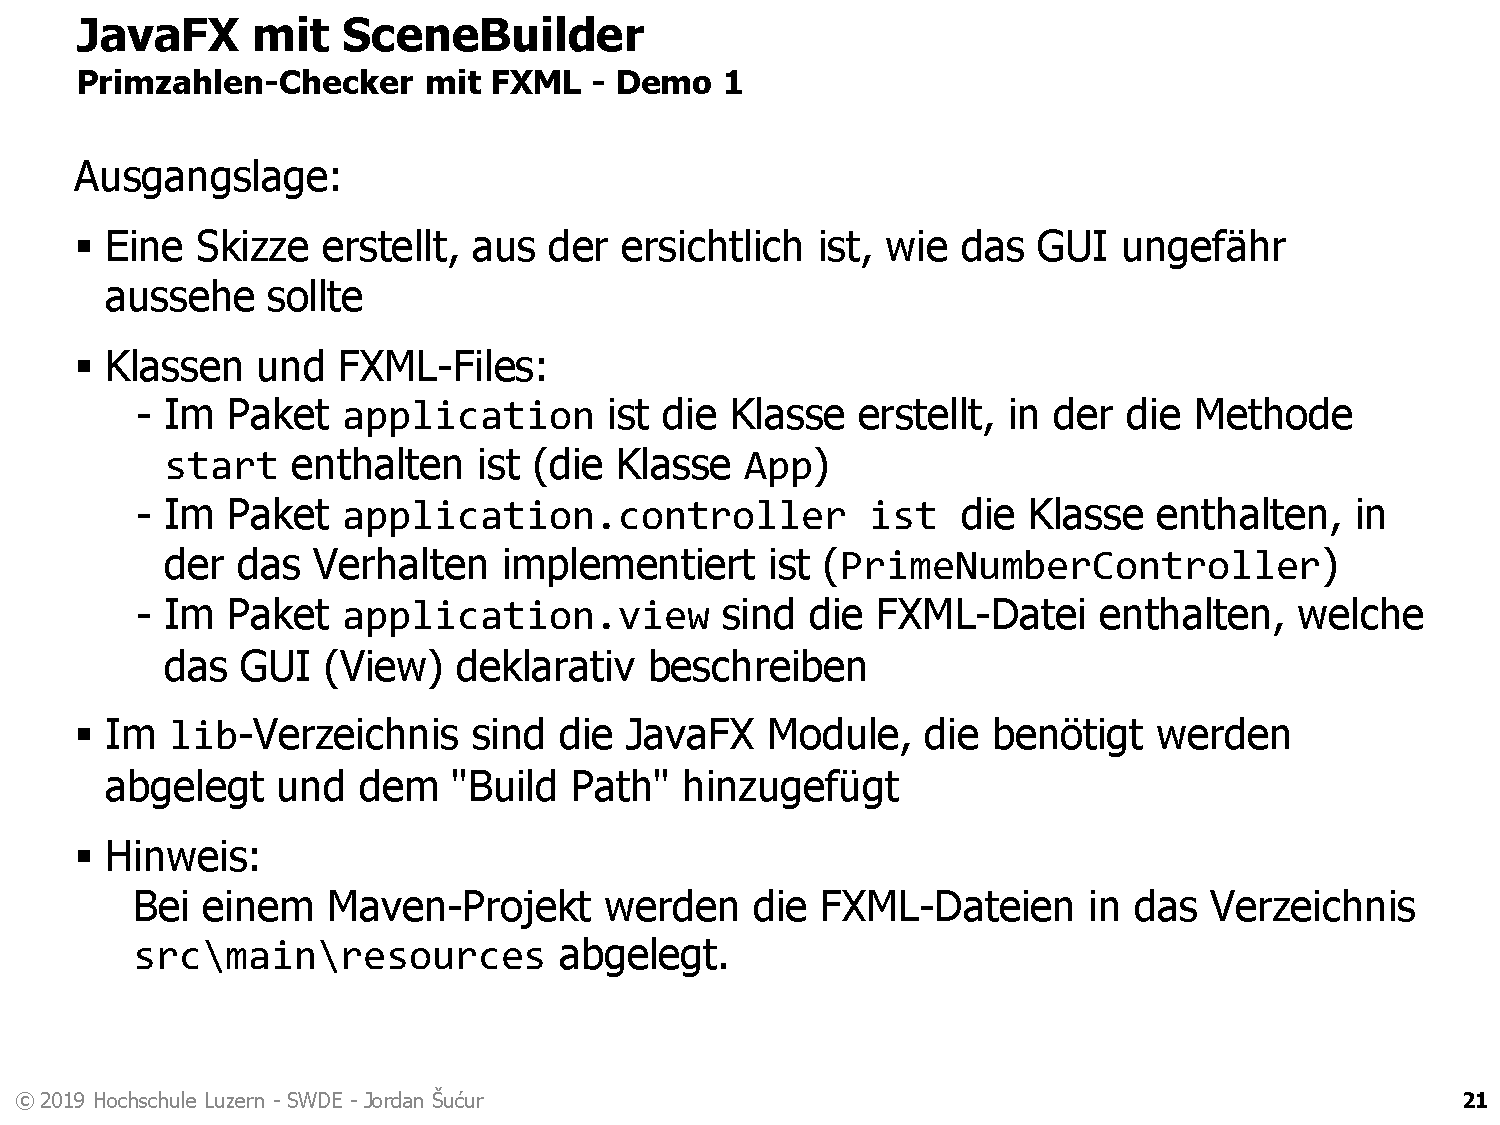
\includepdf[pages=-, pagecommand={}, width=.8\textwidth, nup=1x3]{pdf/javafx.pdf}
		
		
\end{document}